% A LaTeX template for MSc Thesis submissions to 
% Politecnico di Milano (PoliMi) - School of Industrial and Information Engineering
%
% S. Bonetti, A. Gruttadauria, G. Mescolini, A. Zingaro
% e-mail: template-tesi-ingind@polimi.it
%
% Last Revision: October 2021
%
% Copyright 2021 Politecnico di Milano, Italy. NC-BY

\documentclass{Configuration_Files/PoliMi3i_thesis}

%------------------------------------------------------------------------------
%	REQUIRED PACKAGES AND  CONFIGURATIONS
%------------------------------------------------------------------------------

% CONFIGURATIONS
\usepackage{parskip} % For paragraph layout
\usepackage{setspace} % For using single or double spacing
\usepackage{emptypage} % To insert empty pages
\usepackage{multicol} % To write in multiple columns (executive summary)
\setlength\columnsep{15pt} % Column separation in executive summary
\setlength\parindent{0pt} % Indentation
\raggedbottom  

% PACKAGES FOR TITLES
\usepackage{titlesec}
% \titlespacing{\section}{left spacing}{before spacing}{after spacing}
\titlespacing{\section}{0pt}{3.3ex}{2ex}
\titlespacing{\subsection}{0pt}{3.3ex}{1.65ex}
\titlespacing{\subsubsection}{0pt}{3.3ex}{1ex}
\usepackage{color}

% PACKAGES FOR LANGUAGE AND FONT
\usepackage[english]{babel} % The document is in English
\usepackage[utf8]{inputenc} % UTF8 encoding
\usepackage[T1]{fontenc} % Font encoding
\usepackage[11pt]{moresize} % Big fonts

% PACKAGES FOR IMAGES
\usepackage{graphicx}
\usepackage{transparent} % Enables transparent images
\usepackage{eso-pic} % For the background picture on the title page
\usepackage{subfig} % Numbered and caption subfigures using \subfloat.
\usepackage{tikz} % A package for high-quality hand-made figures.
\usetikzlibrary{}
\graphicspath{{./Images/}} % Directory of the images
\usepackage{caption} % Coloured captions
\usepackage{xcolor} % Coloured captions
\usepackage{amsthm,thmtools,xcolor} % Coloured "Theorem"
\usepackage{float}

% STANDARD MATH PACKAGES
\usepackage{amsmath}
\usepackage{amsthm}
\usepackage{amssymb}
\usepackage{amsfonts}
\usepackage{bm}
\usepackage[overload]{empheq} % For braced-style systems of equations.
\usepackage{fix-cm} % To override original LaTeX restrictions on sizes

% PACKAGES FOR TABLES
\usepackage{tabularx}
\usepackage{longtable} % Tables that can span several pages
\usepackage{colortbl}

% PACKAGES FOR ALGORITHMS (PSEUDO-CODE)
\usepackage{algorithm}
\usepackage{algorithmic}

% PACKAGES FOR REFERENCES & BIBLIOGRAPHY
\usepackage[colorlinks=true,linkcolor=black,anchorcolor=black,citecolor=black,filecolor=black,menucolor=black,runcolor=black,urlcolor=black]{hyperref} % Adds clickable links at references
\usepackage{cleveref}
\usepackage{notoccite}
\usepackage[square, numbers, sort&compress]{natbib} % Square brackets, citing references with numbers, citations sorted by appearance in the text and compressed
\bibliographystyle{ieeetr} % You may use a different style adapted to your field
\def\bibfont{\footnotesize}

% OTHER PACKAGES
\usepackage{pdfpages} % To include a pdf file
\usepackage{afterpage}
\usepackage{lipsum} % DUMMY PACKAGE
\usepackage{fancyhdr} % For the headers
\fancyhf{}


% Input of configuration file. Do not change config.tex file unless you really know what you are doing. 
% Define blue color typical of polimi
\definecolor{bluepoli}{cmyk}{0.4,0.1,0,0.4}


% Custom theorem environments
\declaretheoremstyle[
  headfont=\color{black}\normalfont\bfseries,
  bodyfont=\color{black}\normalfont\itshape,
]{colored}

% Set-up caption colors
\captionsetup[figure]{labelfont={color=black}} % Set colour of the captions
\captionsetup[table]{labelfont={color=black}} % Set colour of the captions
\captionsetup[algorithm]{labelfont={color=black}} % Set colour of the captions

\theoremstyle{colored}
\newtheorem{theorem}{Theorem}[chapter]
\newtheorem{proposition}{Proposition}[chapter]

% Enhances the features of the standard "table" and "tabular" environments.
\newcommand\T{\rule{0pt}{2.6ex}}
\newcommand\B{\rule[-1.2ex]{0pt}{0pt}}

% Pseudo-code algorithm descriptions.
\newcounter{algsubstate}
\renewcommand{\thealgsubstate}{\alph{algsubstate}}
\newenvironment{algsubstates}
  {\setcounter{algsubstate}{0}%
   \renewcommand{\STATE}{%
     \stepcounter{algsubstate}%
     \Statex {\small\thealgsubstate:}\space}}
  {}

% New font size
\newcommand\numfontsize{\@setfontsize\Huge{200}{60}}

% Title format: chapter
\titleformat{\chapter}[hang]{
\fontsize{50}{20}\selectfont\bfseries\filright}{\textcolor{bluepoli} \thechapter\hsp\hspace{2mm}\textcolor{bluepoli}{|   }\hsp}{0pt}{\huge\bfseries \textcolor{bluepoli}
}

% Title format: section
\titleformat{\section}
{\color{bluepoli}\normalfont\Large\bfseries}
{\color{bluepoli}\thesection.}{1em}{}

% Title format: subsection
\titleformat{\subsection}
{\color{bluepoli}\normalfont\large\bfseries}
{\color{bluepoli}\thesubsection.}{1em}{}

% Title format: subsubsection
\titleformat{\subsubsection}
{\color{bluepoli}\normalfont\large\bfseries}
{\color{bluepoli}\thesubsubsection.}{1em}{}


% Shortening for setting no horizontal-spacing
\newcommand{\hsp}{\hspace{0pt}}

\makeatletter
% Renewcommand: cleardoublepage including the background pic
\renewcommand*\cleardoublepage{%
  \clearpage\if@twoside\ifodd\c@page\else
  \null
  \AddToShipoutPicture*{\BackgroundPic}
  \thispagestyle{empty}%
  \newpage
  \if@twocolumn\hbox{}\newpage\fi\fi\fi}
\makeatother

%For correctly numbering algorithms
\numberwithin{algorithm}{chapter}

%For costumized list
\newlist{goalist}{itemize}{1}
\setlist[goalist]{label=[\textbf{G1}]}
\newcommand\itemgb{\item[{[\textbf{G2}]}]}
\newcommand\itemgc{\item[{[\textbf{G3}]}]}
\newcommand\itemgd{\item[{[\textbf{G4}]}]}
\newcommand\itemge{\item[{[\textbf{G5}]}]}
\newcommand\itemgf{\item[{[\textbf{G6}]}]}
\newcommand\itemgg{\item[{[\textbf{G7}]}]}
\newcommand\itemgh{\item[{[\textbf{G8}]}]}
\newcommand\itemgi{\item[{[\textbf{G9}]}]}

%For costumized list
\newlist{domainlist}{itemize}{1}
\setlist[domainlist]{label=[\textbf{D1}]}
\newcommand\itemdb{\item[{[\textbf{D2}]}]}
\newcommand\itemdc{\item[{[\textbf{D3}]}]}
\newcommand\itemdd{\item[{[\textbf{D4}]}]}
\newcommand\itemde{\item[{[\textbf{D5}]}]}
\newcommand\itemdf{\item[{[\textbf{D6}]}]}
\newcommand\itemdg{\item[{[\textbf{D7}]}]}
\newcommand\itemdh{\item[{[\textbf{D8}]}]}

\usepackage{listings}
\usepackage{xcolor}

\lstdefinelanguage{alloy}{
  keywords={abstract, sig, extends, var, fact, lone, one, set, always, implies, before, historically, some, all, none, pred, run, in},
  keywordstyle=\color{blue}\bfseries,
  comment=[l]{//},
  commentstyle=\color{green!70!black}\itshape,
  morestring=[b]',
  stringstyle=\color{red},
}

\lstset{
  language=alloy,
  basicstyle=\ttfamily\small,
  keywordstyle=\color{blue}\bfseries,
  commentstyle=\color{green!70!black}\itshape,
  stringstyle=\color{red},
  showstringspaces=false,
  tabsize=2,
  literate={'}{{\textquotesingle}}1
}

%----------------------------------------------------------------------------
%	NEW COMMANDS DEFINED
%----------------------------------------------------------------------------

% EXAMPLES OF NEW COMMANDS
\newcommand{\bea}{\begin{eqnarray}} % Shortcut for equation arrays
\newcommand{\eea}{\end{eqnarray}}
\newcommand{\e}[1]{\times 10^{#1}}  % Powers of 10 notation

%----------------------------------------------------------------------------
%	ADD YOUR PACKAGES (be careful of package interaction)
%----------------------------------------------------------------------------
\usepackage{nomencl}
\makenomenclature
\usepackage{siunitx}
\usepackage{enumitem}

%----------------------------------------------------------------------------
%	ADD YOUR DEFINITIONS AND COMMANDS (be careful of existing commands)
%----------------------------------------------------------------------------

%----------------------------------------------------------------------------
%	BEGIN OF YOUR DOCUMENT
%----------------------------------------------------------------------------

\begin{document}

\fancypagestyle{plain}{%
\fancyhf{} % Clear all header and footer fields
\fancyhead[RO,RE]{\thepage} %RO=right odd, RE=right even
\renewcommand{\headrulewidth}{0pt}
\renewcommand{\footrulewidth}{0pt}}

%----------------------------------------------------------------------------
%	TITLE PAGE
%----------------------------------------------------------------------------

\pagestyle{empty} % No page numbers
\frontmatter % Use roman page numbering style (i, ii, iii, iv...) for the preamble pages

\puttitle{
	title={RASD}, % Title of the thesis
	name=Name, % Author Name and Surname
	advisor= Matteo Camilli , % Supervisor name
    phdcycle = 2024-2025
    %chair={}
} % These info will be put into your Title page 

%----------------------------------------------------------------------------
%	PREAMBLE PAGES: ABSTRACT (inglese e italiano), EXECUTIVE SUMMARY
%----------------------------------------------------------------------------
\startpreamble
\setcounter{page}{1} % Set page counter to 1

%----------------------------------------------------------------------------
%	LIST OF CONTENTS/FIGURES/TABLES/SYMBOLS
%----------------------------------------------------------------------------

% TABLE OF CONTENTS
\setcounter{tocdepth}{3}
\setcounter{secnumdepth}{3}
\tableofcontents % Table of contents 
\thispagestyle{empty}
% LIST OF FIGURES
\listoffigures
\thispagestyle{empty}
% LIST OF TABLES
\listoftables
\thispagestyle{empty}
% LIST OF ABBREVIATIONS AND ACRONYMS
\nomenclature{\(POLIMI\)}{Politecnico di Milano}
\printnomenclature[5em]
\thispagestyle{empty}
\cleardoublepage

%-------------------------------------------------------------------------
%	THESIS MAIN TEXT
%-------------------------------------------------------------------------
% In the main text of your thesis you can write the chapters in two different ways:
%
%(1) As presented in this template you can write:
%    \chapter{Title of the chapter}
%    *body of the chapter*
%
%(2) You can write your chapter in a separated .tex file and then include it in the main file with the following command:
%    \chapter{Title of the chapter}
%    \input{chapter_file.tex}
%
% Especially for long thesis, we recommend you the second option.

\addtocontents{toc}{\vspace{2em}} % Add a gap in the Contents, for aesthetics
\mainmatter % Begin numeric (1,2,3...) page numbering

% --------------------------------------------------------------------------
% NUMBERED CHAPTERS % Regular chapters following
% --------------------------------------------------------------------------

%\chapter{Chapter title}
%\label{chapter:chapter1}
\chapter{Introduction}

\section{Purpose}
As internships become a fundamental part of academic and professional careers, providing students with easier access to opportunities is more important than ever. Traditionally, internship management has relied on fragmented systems, where students struggle to find opportunities, companies face difficulties in attracting the right candidates, and universities have limited visibility into the process.

The Student\&Company (S\&C) Platform aims to bridge these gaps. It provides a centralized system where students can explore internships, enhance their CVs, and apply with ease. Companies benefit by gaining access to tools to improve their internship postings and efficiently manage applications. Meanwhile, universities can monitor the process, mediate issues, and ensure fair practices.

The platform’s primary goals are:
\begin{enumerate}
    \item To simplify and enhance the internship application process for students.
    \item To support companies in attracting and selecting top talent.
    \item To empower universities to oversee and manage complaints effectively.
    \item To foster transparent and effective communication among all stakeholders.
\end{enumerate}

This platform is designed to create a more equitable, efficient, and user-friendly experience for students, companies, and universities, ensuring a collaborative and successful internship process.

S\&C, therefore, intends to serve the following primary goals:

\begin{goalist}
    \item \textbf{Allow students to look for internships and stay updated about new opportunities}
    
        Students can explore various internship opportunities available on the platform and receive notifications about new listings
    
    \itemgb \textbf{Allow students to improve their CVs}
    
        Students can use the platform’s tools and suggestions to improve their CVs, making them more appealing to companies 
    
    \itemgc \textbf{Allow students to apply for an internship}
    
        Students can submit applications for internships directly through the platform, ensuring a seamless and efficient process 
    
    \itemgd \textbf{Allow a company to hire interns}
    
        Companies can use the platform to post internship opportunities, evaluate applications, and select the most suitable candidates for their needs 
    
    \itemge \textbf{Allow companies to improve their internship proposals to attract candidates}
    
        The platform provides feedback and suggestions to help companies refine their internship descriptions, making them more attractive to applicants 
   
    \itemgf \textbf{Allow users to track and monitor the progress of the internship matchmaking process}
    
        Both students and companies can track the progress of their applications or internship postings, gaining insights into the status and next steps 
    
    \itemgg \textbf{Allow users to report issues or raise concerns regarding the internship process}
    
        The platform enables users to flag problems or provide feedback on any aspect of the internship process, ensuring accountability and resolution 
    
    \itemgh \textbf{Allow universities to review and address complaints}
    
       Universities can review and address complaints submitted by students or companies and eventually end the process if necessary. This promotes fairness and transparency throughout the internship process 

\end{goalist}

\section{Scope}

The Students\&Companies (S\&C) platform is designed to facilitate the process of matching university students seeking internships with the companies who offers them. The platform's scope includes providing a centralized, user-friendly interface where students, companies, and universities can interact to support the internship process from start to finish. Key platform features include profile management, internship listings, recommendation system, application processing, complaint handling, and tracking of internship progress.

The platform supports three main actors: Students, Companies, and Universities, each with specific capabilities.

Students use the platform to find internships, and manage applications. They have access to the following functionalities: 
\begin{itemize} 
\item CV Upload and Feedback: Upload CV to receive suggestions on how to improve it making profiles more appealing for internships. 
\item Internship Search and Evaluation: Browse and evaluate internships that match their skills and preferences, with the aid of a recommendation engine that filters opportunities based on keyword matching and statistical criteria. 
\item Internship Application: Apply for internships that meet their qualifications and track application status. 
\item Internship Selection: Review and accept offers from companies based on a structured selection process. 
\item Complaint Submission: Submit complaints if issues arise during the internship, with the ability to track complaint resolution. 
\item Progress Tracking: Monitor the status and progress of ongoing applications and active internships. 
\end{itemize}

Companies use the platform to post internship opportunities, review applicants, and select candidates. The main functionalities include: \begin{itemize} 
\item Internship Posting and Improvement Suggestions: Post detailed internship descriptions, including requirements, skills, and benefits offered. Receive system-generated suggestions to make internship postings more attractive to students. 
\item Student Search and Recommendation: Access a list of student profiles that match internship criteria through keyword search and statistical matching. 
\item Candidate Interviews: Schedule and conduct interviews with suggested candidates and gather feedback. 
\item Candidate Selection: Choose which students to hire based on the interview and selection process. 
\item Complaint Submission: Raise complaints regarding student performance or internship issues and track resolutions. 
\item Internship Management: Track and monitor the status of internships with each student. 
\end{itemize}

Universities oversee and manage the internship process to ensure educational objectives and address complaints. Their primary functionalities include: 
\begin{itemize} 
\item Internship Monitoring: Oversee the internship status and progress of students affiliated with the university, with access to feedback and performance tracking. 
\item Complaint Handling: Review and address complaints, including those that may require the intervention or termination of an internship.
\end{itemize}

Additional Platform Functionalities
\begin{itemize} 
\item ???
\end{itemize}

\subsection{Phenomena}

\begin{table}[H]
    \centering 
    \arrayrulecolor{gray!50} % Imposta il colore delle linee a grigio chiaro
    \begin{tabular}{|p{22em} | c | c |}
    \hline
    \rowcolor{bluepoli!40} 
    \textbf{Title} & \textbf{Controlled by} & \textbf{Shared?} \T\B \\
    \hline \hline
    \textbf{User Registration} & World & Yes\T\B \\
    \hline
    \textbf{User Login} & World & Yes\T\B\\
    \hline
    \textbf{Student insert CV} & World & No \B\\
    \hline
    \textbf{User receive recommendations based on their preferences} & Machine & Yes \B\\
    \hline
    \textbf{Companies offer new internship} & World & No\B\\
    \hline
    \textbf{System provides suggestions to improve CVs and project description} & Machine & Yes\B\\
    \hline
    \textbf{Students apply for internship} & World  & Yes\B\\
    \hline
    \textbf{System collects statistics} & Machine & No \B\\
    \hline
    \textbf{Companies approve application} & World & No\B\\
    \hline
    \textbf{Companies interview students} & World & Yes\B\\
    \hline
    \textbf{Universities monitor internships} & World & No\B\\
    \hline
    \textbf{User monitor the outcome of the matchmaking} & World  & /\B\\
    \hline
    \textbf{Notify students when an internship that might interest them becomes available} & Machine  & Yes\B\\
    \hline
    \textbf{Students accepts internship} & World  & /\B\\
    \hline
    \textbf{Notify companies about the availability of student CVs corresponding to their needs} & Machine & Yes\B\\
    \hline
    \textbf{Systems asks students and companies to provide feedback and suggestions} & Machine & Yes\B\\
    \hline
    \textbf{Students visualize final outcome of the internship} & / & Yes\B\\
    \hline
    \textbf{System updates the status of the matchmaking} & Machine  & No\B\\
    \hline
    \textbf{User visualizes the status of the matchmaking} & /  & /\B\\
    \hline
    \textbf{Company accepts application} & / & /\B\\
    \hline
    \textbf{Universities handles complaints} & /  & /\B\\
    \hline
    \textbf{University interrupts the internship} & /  & /\B\\
    \hline
    \textbf{Systems removes expired or accepted internships} & /  & /\B\\
    \hline
    \end{tabular}
    \\[10pt]
    \caption{Phenomena}
    \label{table:example}
\end{table}


\section{Definitions, Acronyms, Abbreviations}

\subsection{Definitions}

\subsection{Acronyms}

\subsection{Abbreviations}

\section{Revision history}

\section{Reference Documents}

\section{Document Structure}

\chapter{Overall description}

\section{Product perspective}

\subsection{Scenarios}

In the following chapter, we present a hypothetical scenario to better illustrate the phenomenon:

\begin{itemize}[leftmargin=*, label={}]
    \item \textbf{Quahog Innovation Company inserts an internship:}
    \begin{itemize}
        \item The Quahog Innovation Company, a leader in Integrating AI into different infrastructures, seeks interns who can bring fresh perspectives to their research. Upon learning about the S\&C platform, they decide to list their internship opportunity there, hoping to attract enthusiastic candidates eager to collaborate. 
    \end{itemize}

    \item \textbf{Quahog Innovation Company improves its internship proposal:}
    \begin{itemize}
        \item As this is the first time the Quahog  Innovation Company is offering an internship, they are unsure how appealing their proposal might be. They follow the platform's suggestions to post first and then enhance their posting, aiming to make it more attractive to potential applicants.
    \end{itemize}

    \item \textbf{Stewie registers on the platform:}
    \begin{itemize}
        \item Stewie, a master’s student at Cleveland University, needs an internship related to his field of study to support his thesis. After discovering the S\&C platform, he decides to use it to find opportunities. He follows the app’s guidance to make his CV and personal account. In the end, he is not convinced about the attractiveness of his curriculum and decides to improve it by following the platform’s guidance to make it more compelling.
    \end{itemize}

    \item \textbf{Stewie applies for an internship:}
    \begin{itemize}
        \item  Once satisfied with the improvements, he starts applying to several internships that not only match his academic background but also fit his interests and long-term career goals, hoping to gain valuable experience that will support his thesis and future aspirations.
    \end{itemize}

    \item \textbf{Quahog Innovation Company analyses the applications received:}
    \begin{itemize}
        \item After receiving multiple applications, the Quahog  Innovation Company begins evaluating candidates. They first filter out applicants who do not meet the prerequisites. Next, they assess the level of interest shown by the remaining candidates, ultimately shortlisting those they believe would bring the greatest value to their organization and match them.
    \end{itemize}

    \item \textbf{Stewie Checks the Status of His Applications:}
    \begin{itemize}
        \item Stewie monitors his applications and finds that while some companies have shown no interest, others have matched him. He also received notifications about new internship opportunities. However, he chooses to proceed with the companies that have expressed interest in his application, as they align better with his aspirations.
    \end{itemize}

    \item \textbf{The company evaluates and interviews applicants:}
    \begin{itemize}
        \item To finalize their decision, the company interviews the students through a structured questionnaire for each specific internship proposed, which all shortlisted candidates have to answer if accepted. In order to make a more The interview delves into the technical knowledge required for the role and asks personal questions about their motivations and goals. Candidates respond to the questionnaire through the platform, providing the company with deeper insights.
    \end{itemize}

    \item \textbf{Stewie receives the questionnaire and answers it}
    \begin{itemize}
        \item Stewie while checking the status of his application notices that the one to Quohag Company was positively evaluated and a questionnaire was available to be answered. Excited about the news, Stewie immediately answers all the questions present and sends back the questionnaire, hoping that the company will continue to show interest in him. 
    \end{itemize}

    \item \textbf{The company evaluates the questionnaires and hires the interns:}
    \begin{itemize}
        \item After reviewing the questionnaires submitted, Quahog Innovation Company identifies candidates who demonstrate technical skills and a passion for AI integration. Following a thorough evaluation, the company shortlists the candidates they want to hire, including Stewie.
    \end{itemize}

    \item \textbf{Stewie accepts the position and starts working in the company:}
    \begin{itemize}
        \item Stewie receives a notification stating that his questionnaire was evaluated positively and that if interested would be contacted by the company with the messaging system available on the platform. Extremely excited, he accepts and gets contacted by the company to clarify all the final information needed before finally starting his experience at Quohag company.
    \end{itemize}

    \item \textbf{Complaints handling:}
    \begin{itemize}
        \item After starting to work at the company, Stewie noticed a few issues with his internship. As time passes, instead of engaging in meaningful work that aligned with his skills and interests, he was assigned only trivial tasks that seemed far beneath his aspirations. Frustrated by the lack of stimulation, Stewie raises a complaint on the S\&C platform. The Cleveland University administration steps in to mediate, contacting the company to address the issue. Prompted by the intervention, the company apologizes and puts Stewie on a new project much closer to his field of interest.
    \end{itemize}
        
    \item \textbf{Finalizing the decision:}
    \begin{itemize}
        \item With the issues resolved, Stewie feels reassured and continues the internship. Excited to start this new project, he leaves a good review on the platform and looks forward to contributing to the company’s innovative projects while gathering valuable information for his thesis and academic growth.
    \end{itemize}
\end{itemize}


\subsection{Domain Class Diagram}

\begin{figure} [H]
    \centering
    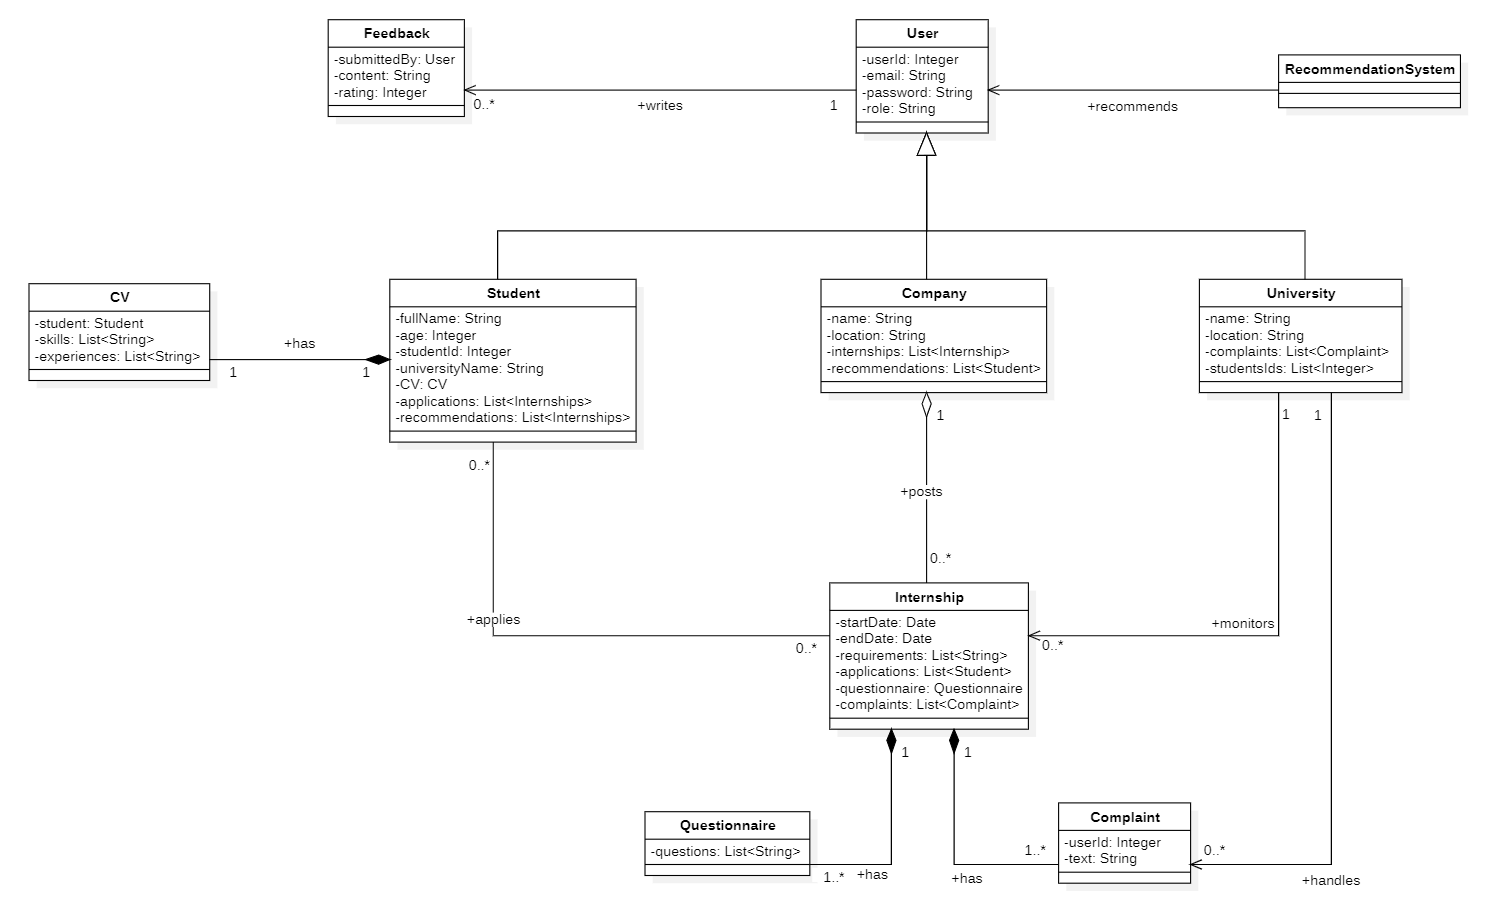
\includegraphics[width=1\linewidth]{Images/domain_class_diagram.png}
    \caption{High level Class Diagram}
    \label{fig: High level Class Diagram}
\end{figure}

\section{Product Functions}

The S\&C platform provides a range of functionalities designed to support the internship matching process for students and companies, oversighted by universities. The main functionalities are described below.

\subsubsection*{User Registration} 
This functionality allows students, companies, and universities to sign up to the S\&C platform and create their profiles.
\begin{itemize}
    \item \textbf{User}: Each user selects their type (student, company, or university) and provides the required information to complete the registration process, such as email, password, and other relevant details.
\end{itemize}

\subsubsection*{Profile Management} 
This functionality enables users to manage and enhance their profiles to increase the likelihood of successful matches.
\begin{itemize}
    \item \textbf{Profile Updates}: Students and companies can update their personal information to complete their profiles after registration.
    \item \textbf{CV Creation}: Students can generate their CVs by providing details about their skills, personal experiences, and other relevant information.
\end{itemize}

\subsubsection*{Enhancement Suggestions}
This feature helps both students and companies improve their profiles and increase their chances to make themselves more appealing to potential matches.
\begin{itemize}
    \item \textbf{CV Improvement}: Students can request suggestions from the system to improve their CVs.
    \item \textbf{Internship Improvement}: Companies can request suggestions from the system to enhance their internship proposals.
    \item \textbf{Questionnaire Improvement}: Companies can request suggestions to improve their questionnaires.
\end{itemize}

\subsubsection*{Internship Posting and Search} 
The platform allows companies to post internships and students to search for opportunities.
\begin{itemize}
    \item \textbf{Internship Creation}: Companies can create detailed internship listings by specifying requirements, skills needed, tasks, compensation, and benefits.
    \item \textbf{Internship Search and Filtering}: Students can browse and filter internships based on criteria such as required skills, duration, location, and compensation.
    \item \textbf{Internship Details View}: Students can thoroughly view details about each internship to assess compatibility with their skills and interests.
\end{itemize}

\subsubsection*{Application and Selection Process} 
This functionality manages applications and the selection process.
\begin{itemize}
    \item \textbf{Application Submission}: Students can apply to internships directly from the listings and track the status of their applications.
    \item \textbf{Candidate Shortlisting}: Companies can review applications, filter candidates based on qualifications, and shortlist those who meet their requirements.
    \item \textbf{Interview Coordination}: Companies can arrange interviews with shortlisted candidates by using questionnaires.
    \item \textbf{Final Selection and Offer Acceptance}: Companies can send offers to selected students, who can accept or decline the offers through the platform.
\end{itemize}

\subsubsection*{Recommendation System} 
The S\&C platform provides a recommendation system to facilitate suitable matches between students and internships.
\begin{itemize}
    \item \textbf{Internship Recommendations for Students}: The platform recommends internships to students based on their profiles.
    \item \textbf{Candidate Recommendations for Companies}: Companies receive recommendations of students whose profiles align with their internship requirements, enabling quick identification of potential matches.
    \item \textbf{Feedback-Driven Refinements}: Both students and companies can provide feedback on recommendations, helping to improve the accuracy and relevance of future matches.
\end{itemize}

\subsubsection*{Complaint Management}
This functionality supports complaint management to address issues and maintain the quality of the internship process.
\begin{itemize}
    \item \textbf{Complaint Submission}: Students and companies can submit complaints if issues arise during internships. Complaints are logged, tracked, and managed through the appropriate channels.
    \item \textbf{University Intervention}: Universities are notified of complaints and can intervene when necessary, including taking action to resolve or terminate internships if needed.
\end{itemize}

\subsubsection*{Progress Tracking} 
This feature allows students, companies, and universities to monitor the progress of applications and active internships.
\begin{itemize}
    \item \textbf{Application Status Updates}: Students and companies can view and track the status of each application, from submission to final selection.
    \item \textbf{Internship Progress Monitoring}: Once an internship begins, students and companies can monitor ongoing activities and report any issues.
    \item \textbf{University Oversight}: Universities can track students’ progress in internships to ensure educational compliance and student welfare.
\end{itemize}

\subsubsection*{Notification System} 
The notification system keeps users informed of critical events and updates.
\begin{itemize}
    \item \textbf{Application and Selection Notifications}: Students are notified of changes in application status, such as interview invitations or selection decisions.
    \item \textbf{Recommendation Alerts}: Students and companies receive alerts for recommended internships or candidate profiles that match their preferences.
    \item \textbf{Complaint and Resolution Updates}: Notifications are sent to relevant parties when complaints are filed or resolved, ensuring transparent communication.
    \item \textbf{Reminder and Follow-Up Alerts}: The system sends reminders for upcoming interviews, deadlines, and other key events to keep users engaged and informed.
\end{itemize}

In summary, the S\&C platform provides a structured, streamlined approach to managing the internship application process from start to finish, including registration, profile management, recommendations, application handling, feedback collection, and progress tracking. This section outlines the essential product functions, organized by feature, providing a clear view of the platform’s primary capabilities.




\section{User characteristics}

\subsubsection*{Student}
The student is a person who studies at a university and is interested in applying for and participating in an internship offered by a company. For this reason, they register on the S\&C platform, where they can find internships either through an active search or via recommendations. After applying, they must pass an interview with the company offering that position. Once the internship begins, the student can communicate any issues or provide updates to both the university and the company using a chat or a form feature.
\subsubsection*{Company}
The company is interested in hiring students through an internship program. It can post work opportunities on the platform, where students can view them. Afterward, the company can receive feedback from the system to support the recruitment process. Once the student is selected, the company may use the platform to send feedback and file complaints to other users during the internship period.
\subsubsection*{University}
The university is the institution where the student studies. It can review and manage complaints submitted by other users and may decide to interrupt the internship based on these considerations.


\section{Assumptions, dependencies and constraints}

\subsubsection*{Domain Assumptions}
The following assumptions are properties and conditions that the system will take for granted. These assumptions are necessary to ensure the correct behaviour of the platform and to achieve its intended goals.
\begin{domainlist}
    \item User must consent to personal data extraction and usage
    \itemdb User must consent to receiving information
    \itemdc Users must provide correct personal
    information at the moment of registration
    \itemdd Student must be enrolled in a university
    \itemde Company must provide correct and clear information about the internships
    \itemdf Student can do only one internship at a time 
    \itemdg University must have students who are actively enrolled in its programs.

\end{domainlist}

\chapter{Specific Requirements}

\section{External Interface Requirements}

\subsection{User Interfaces}


This initial illustration depicts the platform's homepage, where users can choose to log in or sign up. [Figure \ref{fig:Landing Page}]

\begin{figure}[H]
    \centering
    
\includegraphics[width=0.5\linewidth]{Interface Images//log in sing up/image.png}
    \caption{Landing Page}
    \label{fig:Landing Page}
\end{figure}

The following page shows a description of the platform's objectives after a user signs up. [Figure \ref{fig:Introduction Page}]

\begin{figure} [H]
    \centering
    
\includegraphics[width=0.5\linewidth]{Interface Images/log in sing up/Screenshot 2024-12-04 115134.png}
    \caption{Introduction Page}
    \label{fig:Introduction Page}
\end{figure}

After a user decides to create an account, they will be asked their role as either a student, company or a university. [Figure \ref{fig:Choice page}] 

\begin{figure} [H]
    \centering
    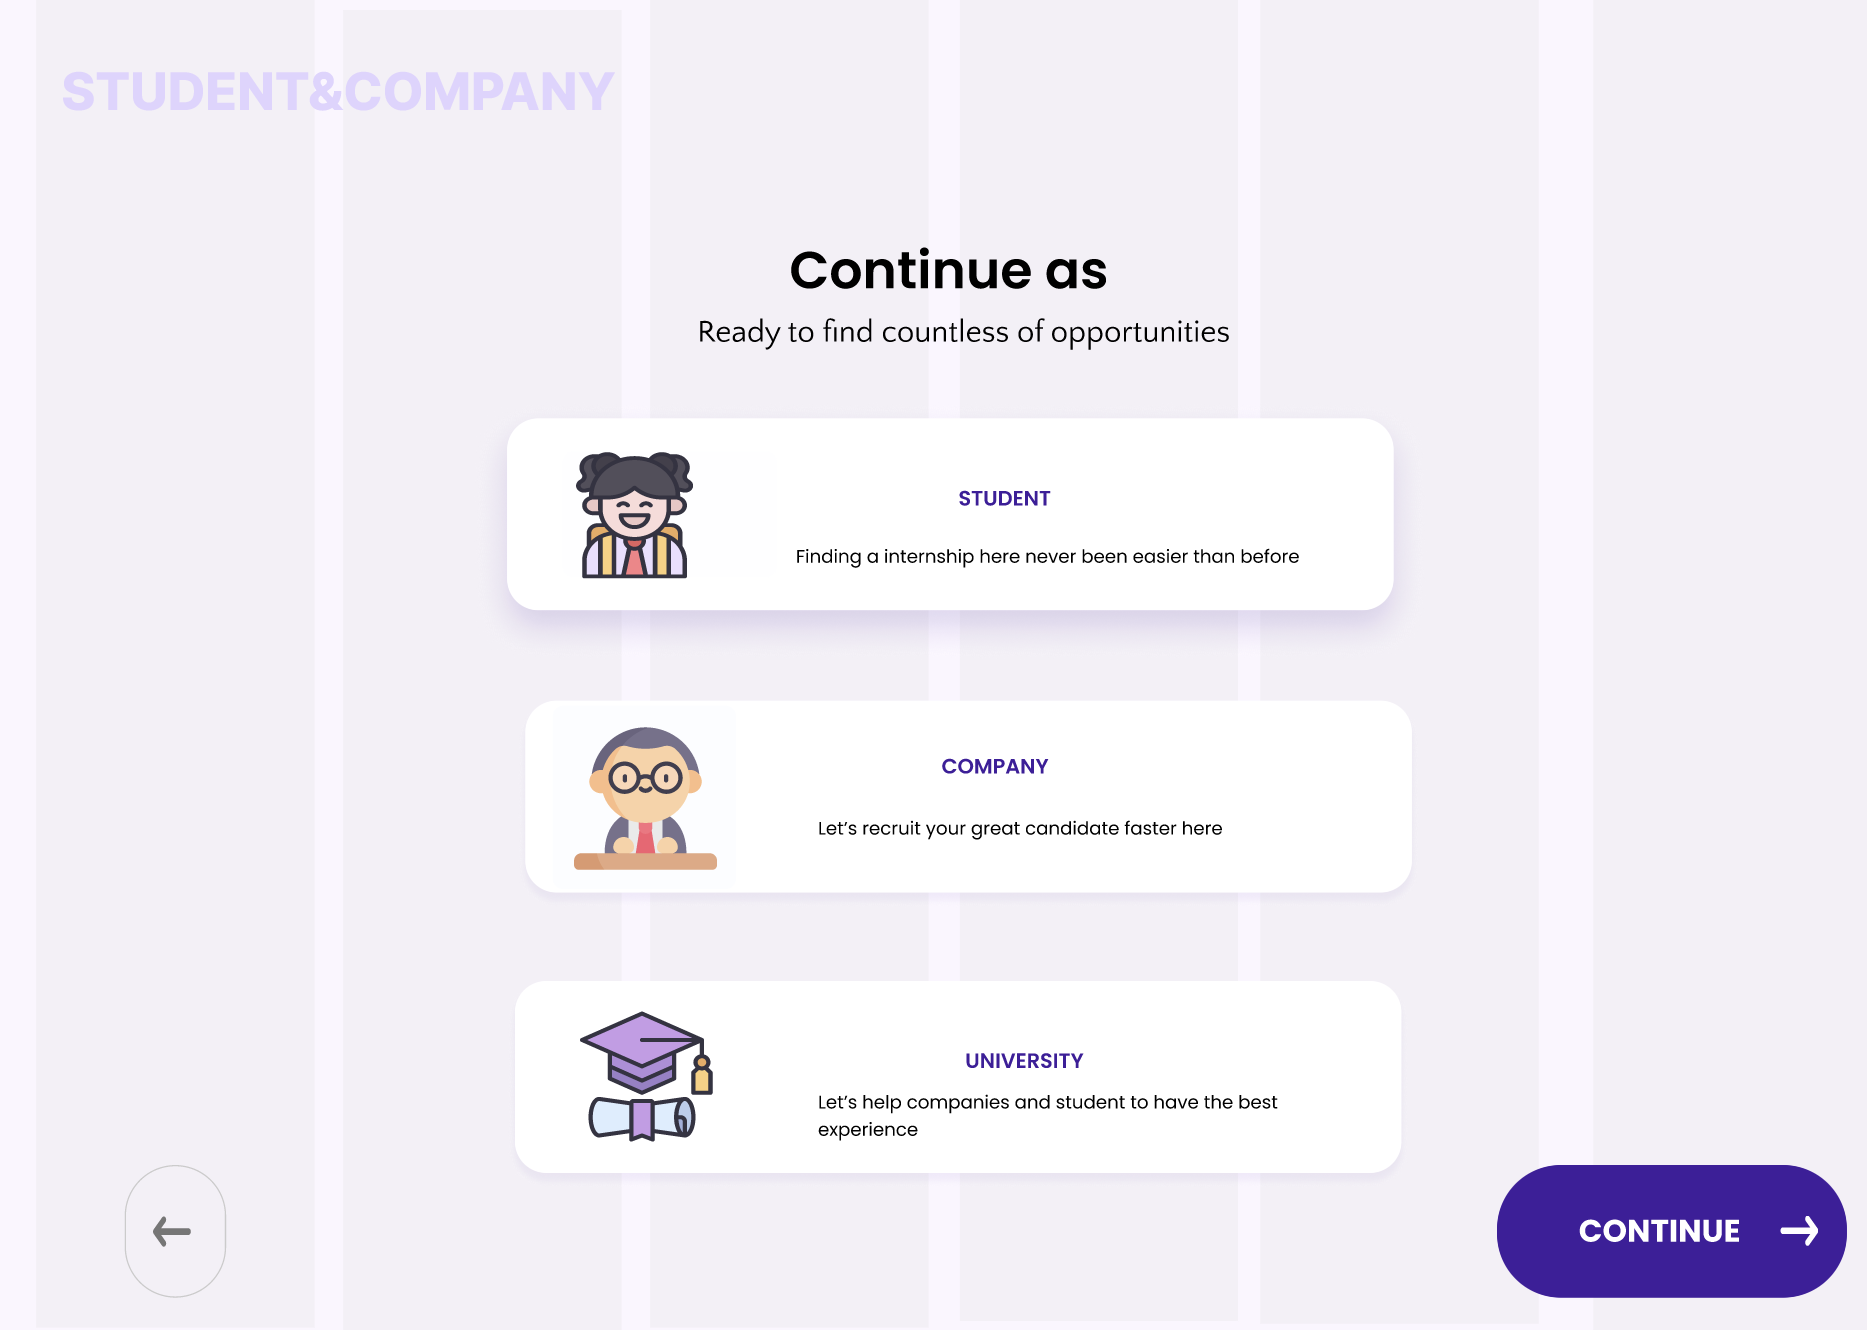
\includegraphics[width=0.5\linewidth]{Interface Images/log in sing up/Screenshot 2024-12-03 110046.png}
    \caption{Choice page}
    \label{fig:Choice page}
\end{figure}

Depending on the role decided by the user, they will be prompted to input various information that can vary based on the specific role. [Figures \ref{fig:Create account for Students}, \ref{fig: Create account for companies}, \ref{fig:Create account for Universities}] 

\begin{figure} [H]
    \centering
    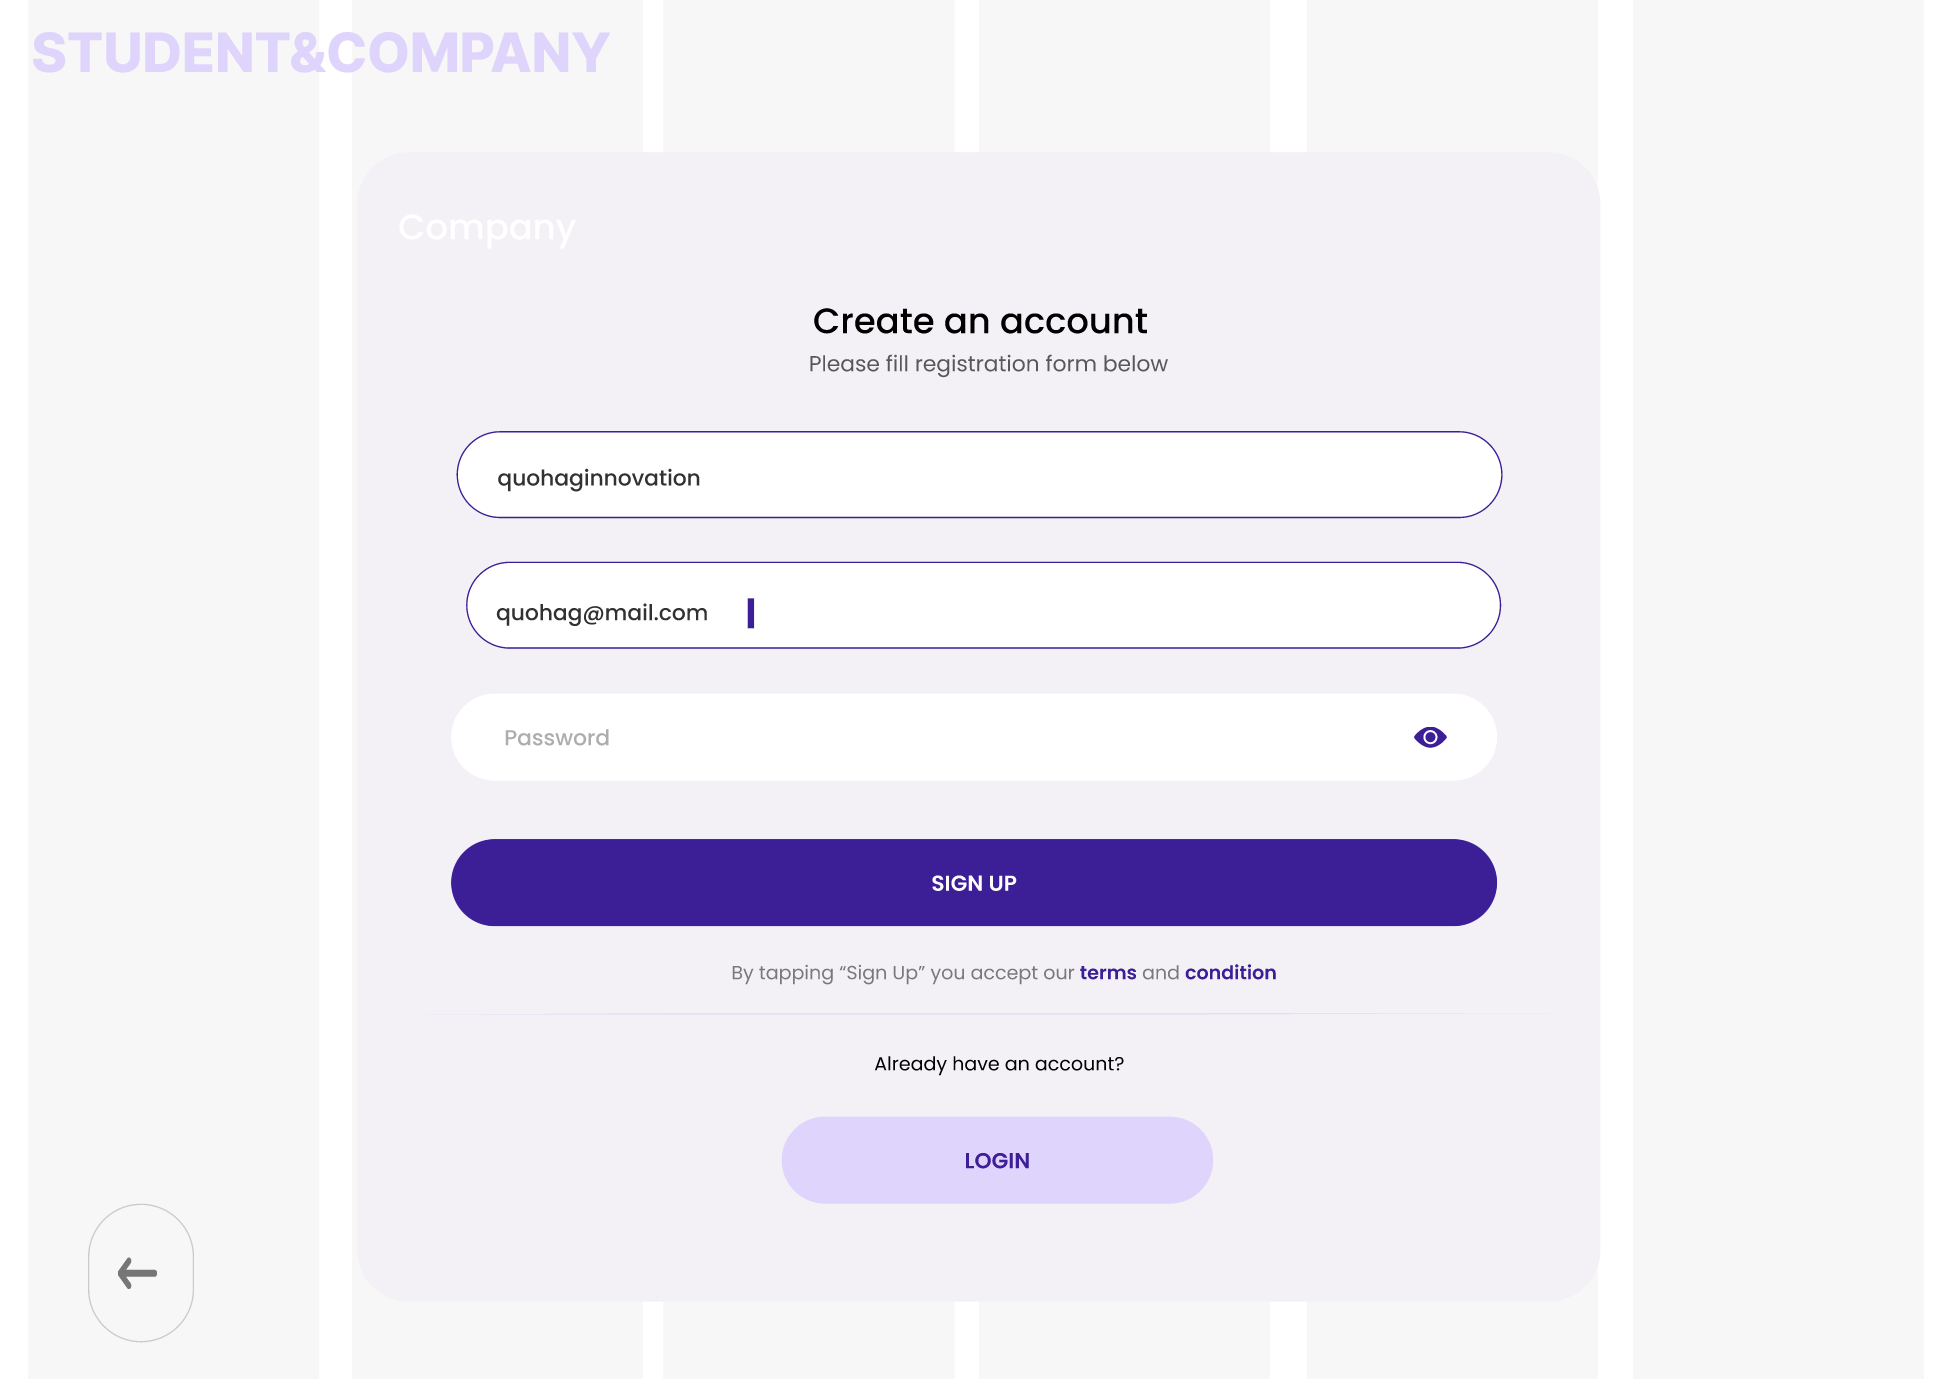
\includegraphics[width=0.5\linewidth]{Interface Images/log in sing up/Screenshot 2024-12-12 045014.png}
    \caption{Create account for Companies }
    \label{fig: Create account for companies}
\end{figure}

\begin{figure} [H]
    \centering
    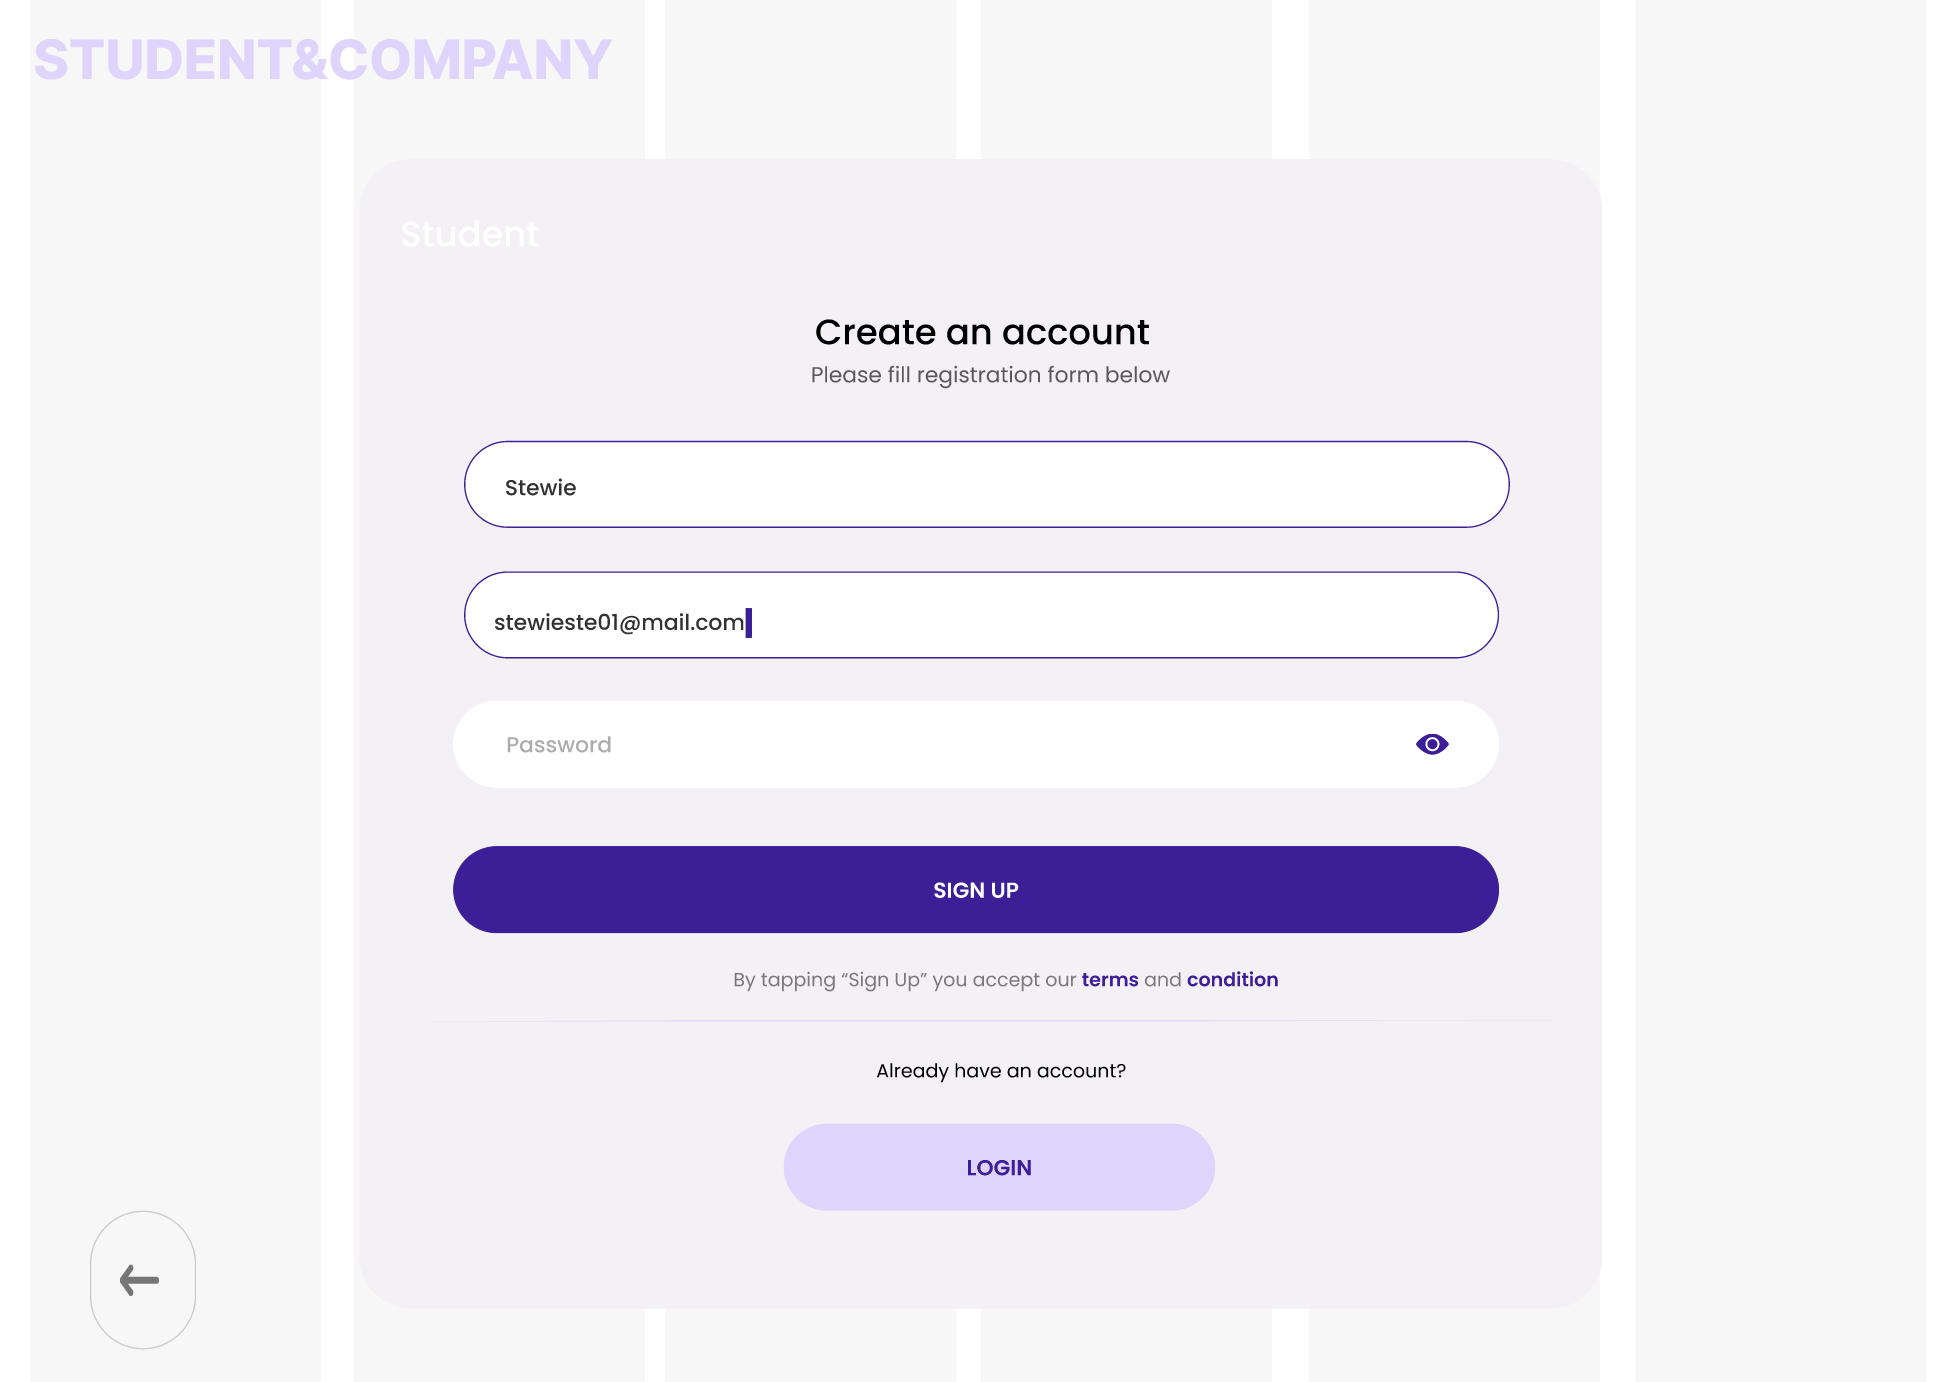
\includegraphics[width=0.5\linewidth]{Interface Images/log in sing up/Screenshot 2024-12-12 045029.png}
    \caption{Create account for Students}
    \label{fig:Create account for Students}
\end{figure}

\begin{figure} [H]
    \centering
    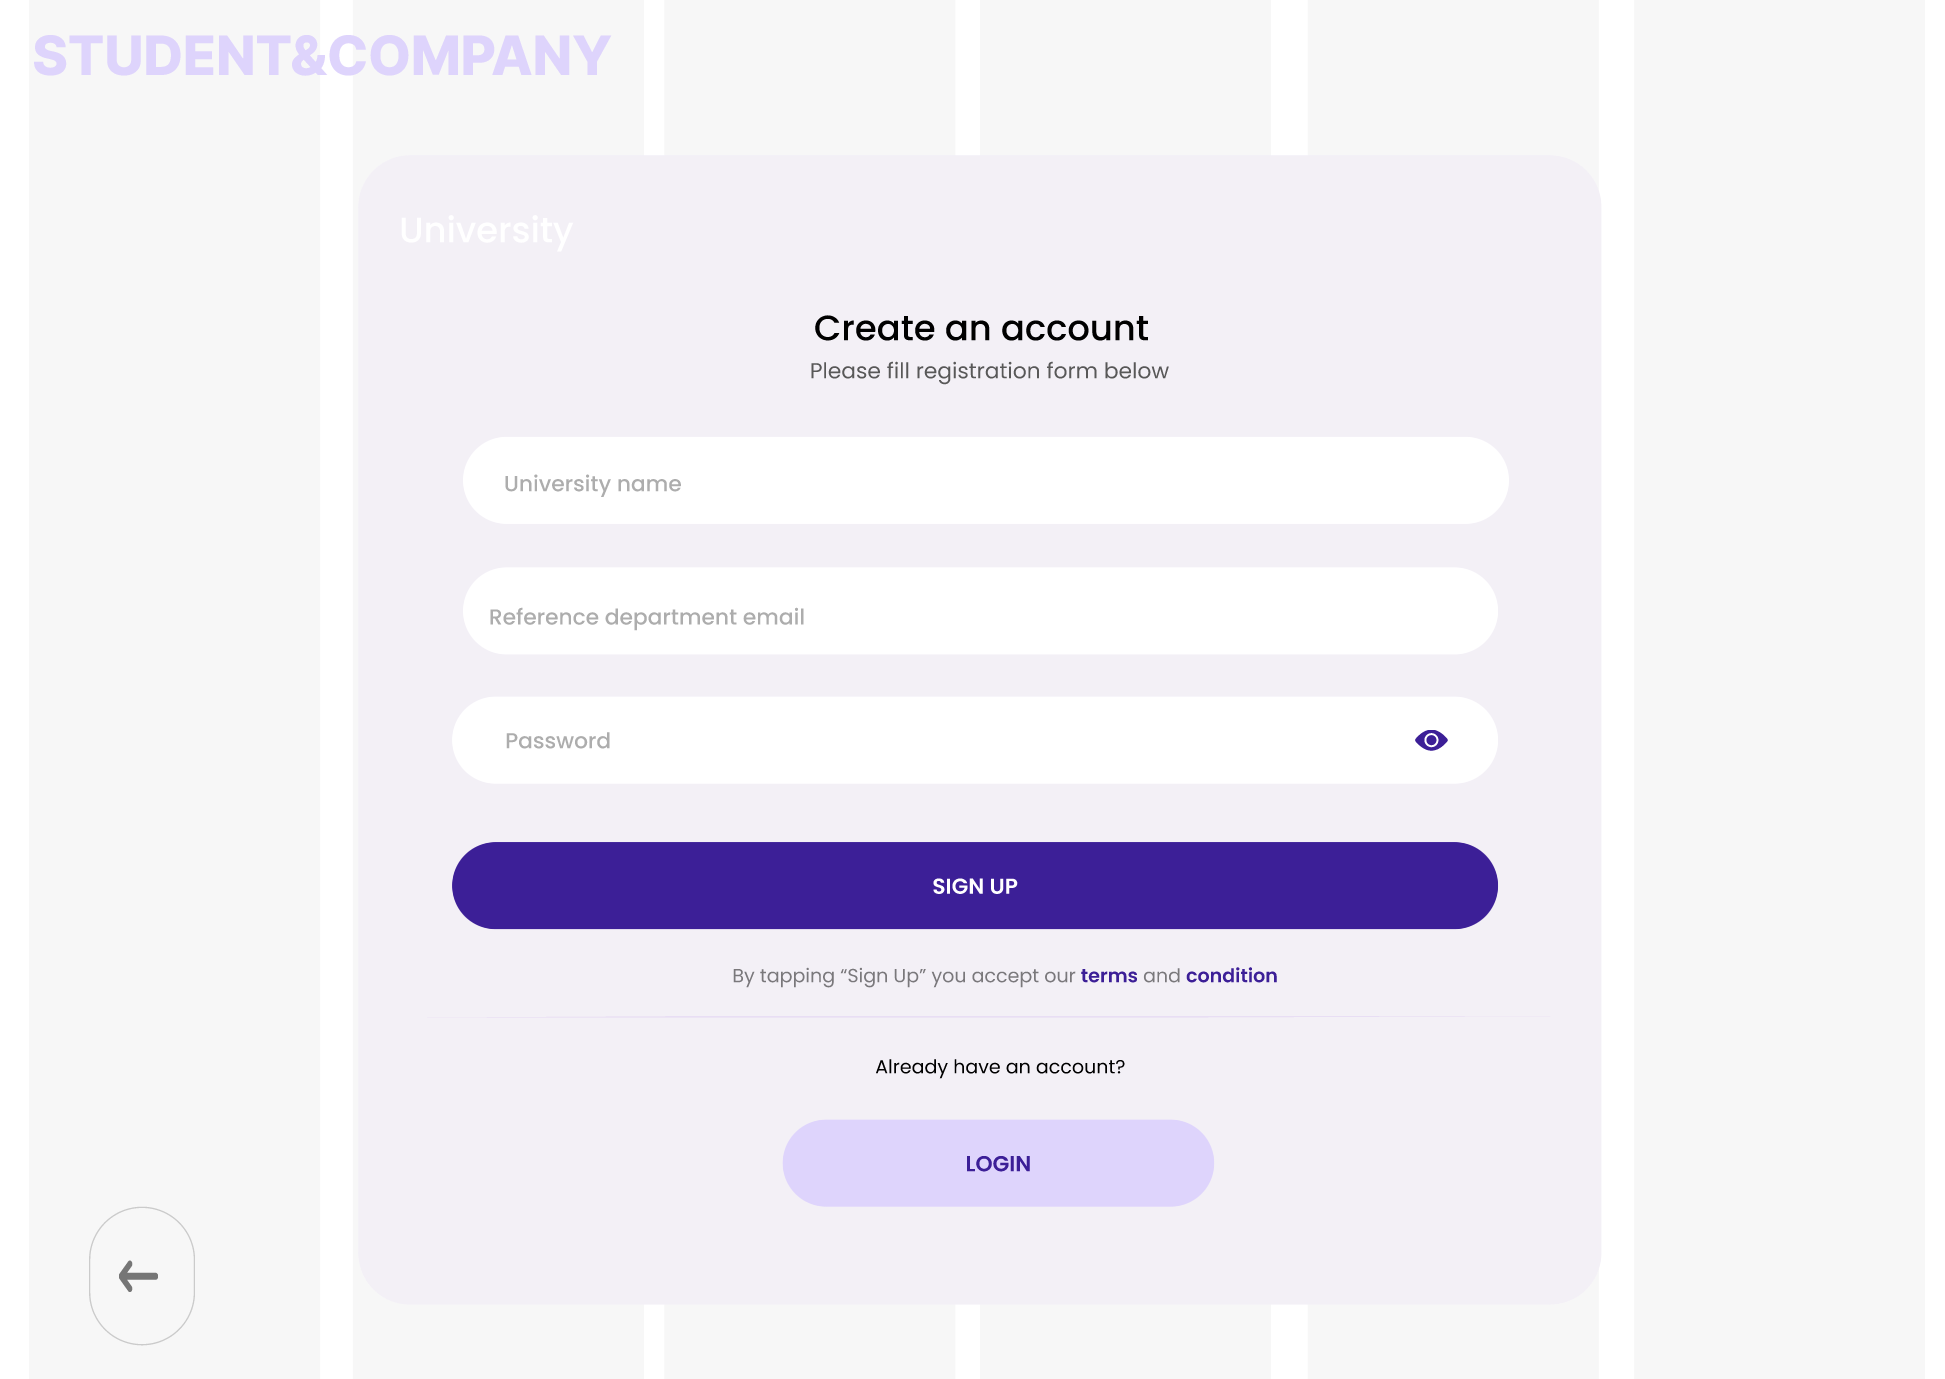
\includegraphics[width=0.5\linewidth]{Interface Images/log in sing up/Screenshot 2024-12-12 045042.png}
    \caption{Create account for Universities}
    \label{fig:Create account for Universities}
\end{figure}

Users with an existing account can access the platform by clicking the appropriate button on the homepage, which directs them to the login page. From there, they can log in using their username and password or by signing in with their Google or Facebook account. If a user mistakenly selects the login option without having an account, they can simply click the "Create Account" button to navigate to the registration page. [Figures \ref{fig:Company Sign in}, \ref{fig: Student Sign in}, \ref{fig:University Sign in}]

\begin{figure} [H]
    \centering
    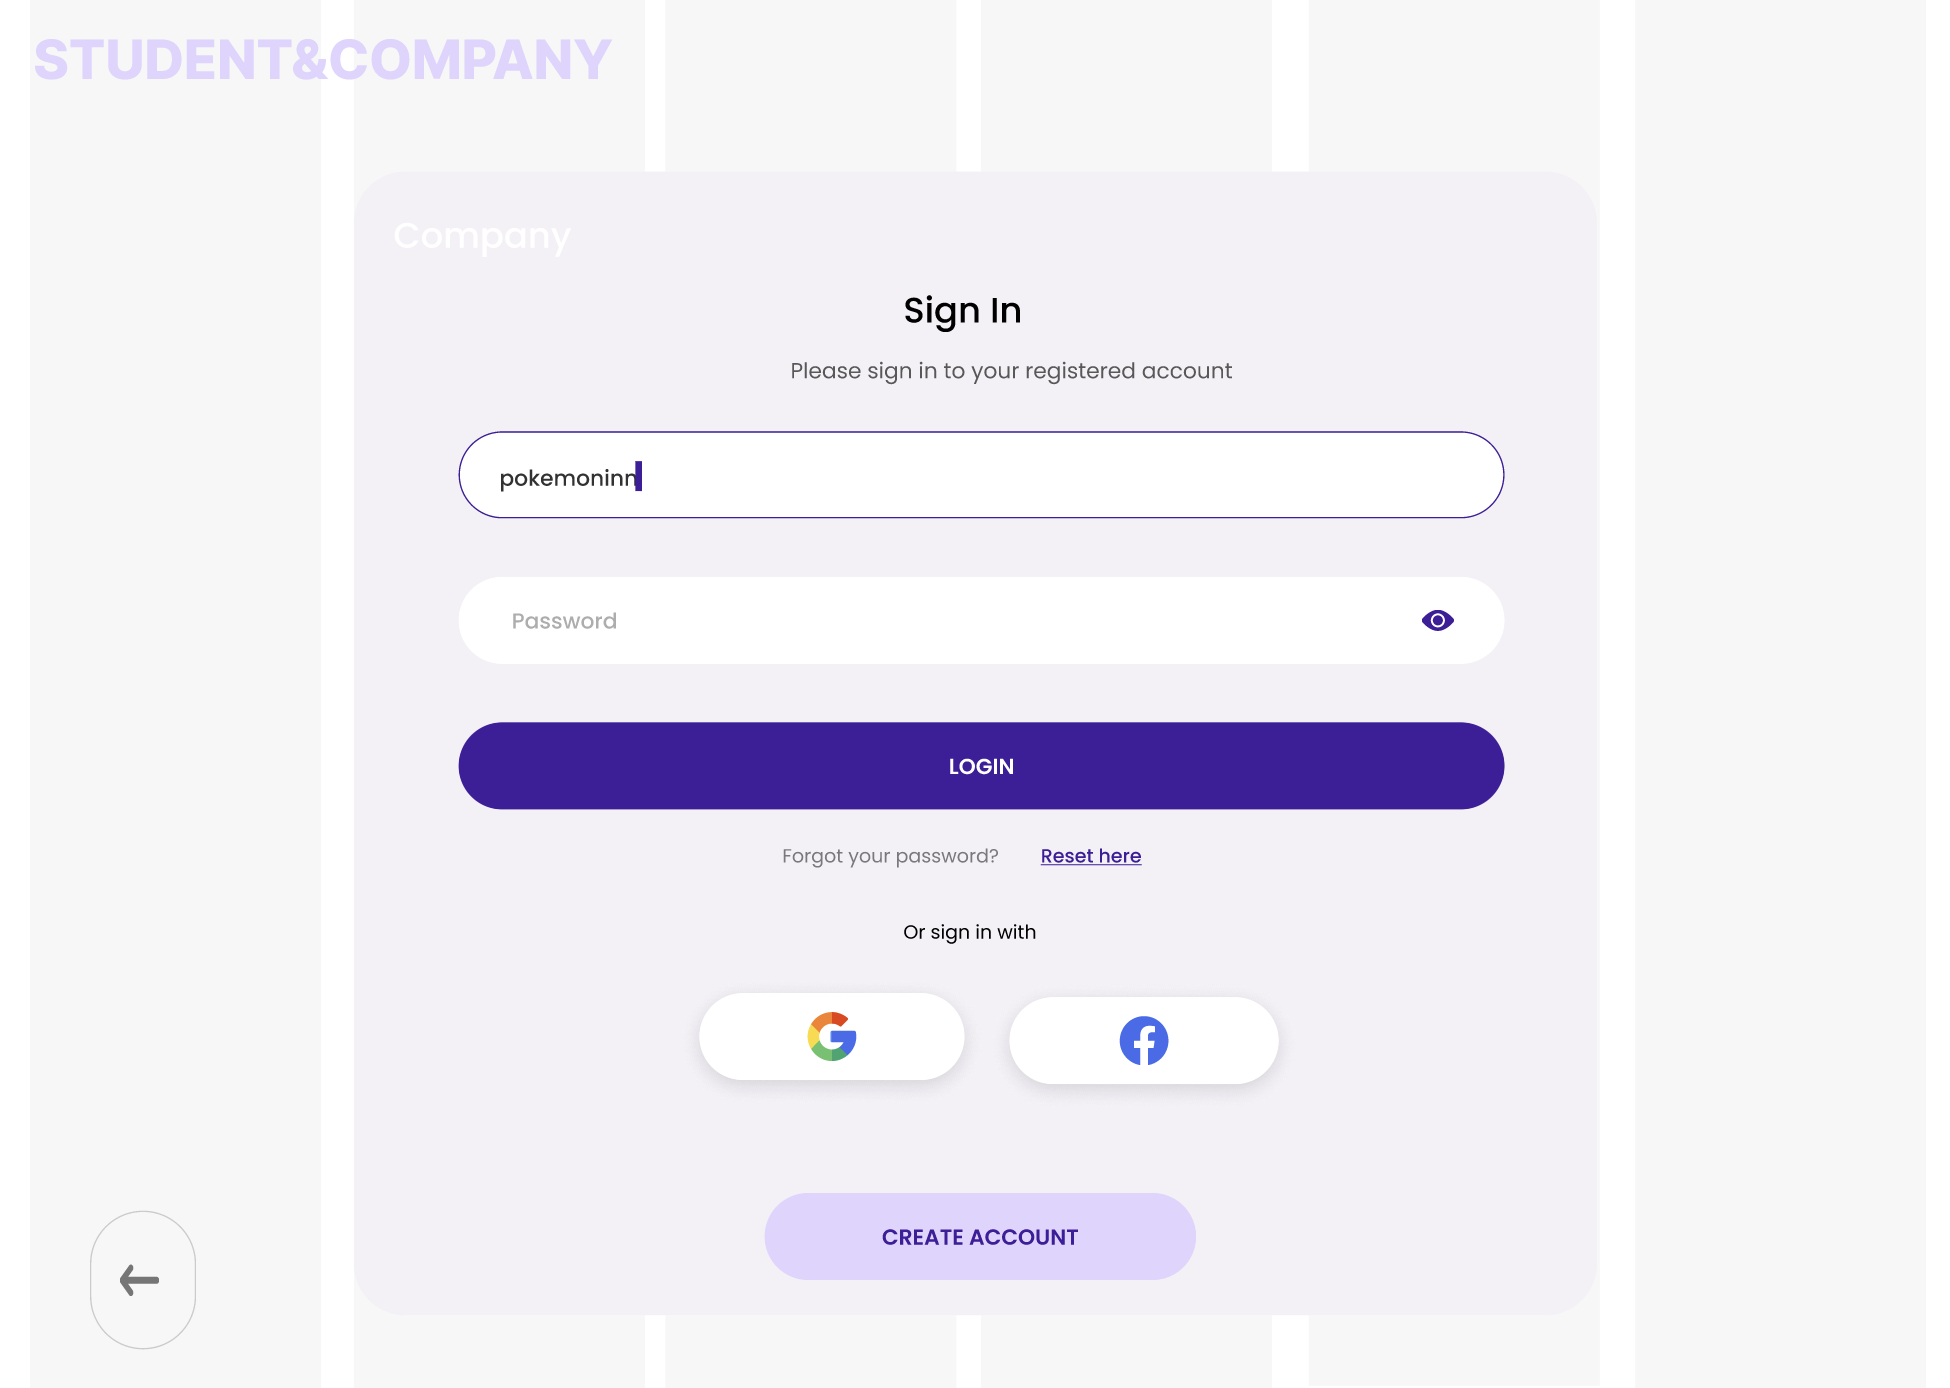
\includegraphics[width=0.5\linewidth]{Interface Images/log in sing up/Screenshot 2024-12-12 045111.png}
    \caption{Company Sign in}
    \label{fig:Company Sign in}
\end{figure}

\begin{figure} [H]
    \centering
    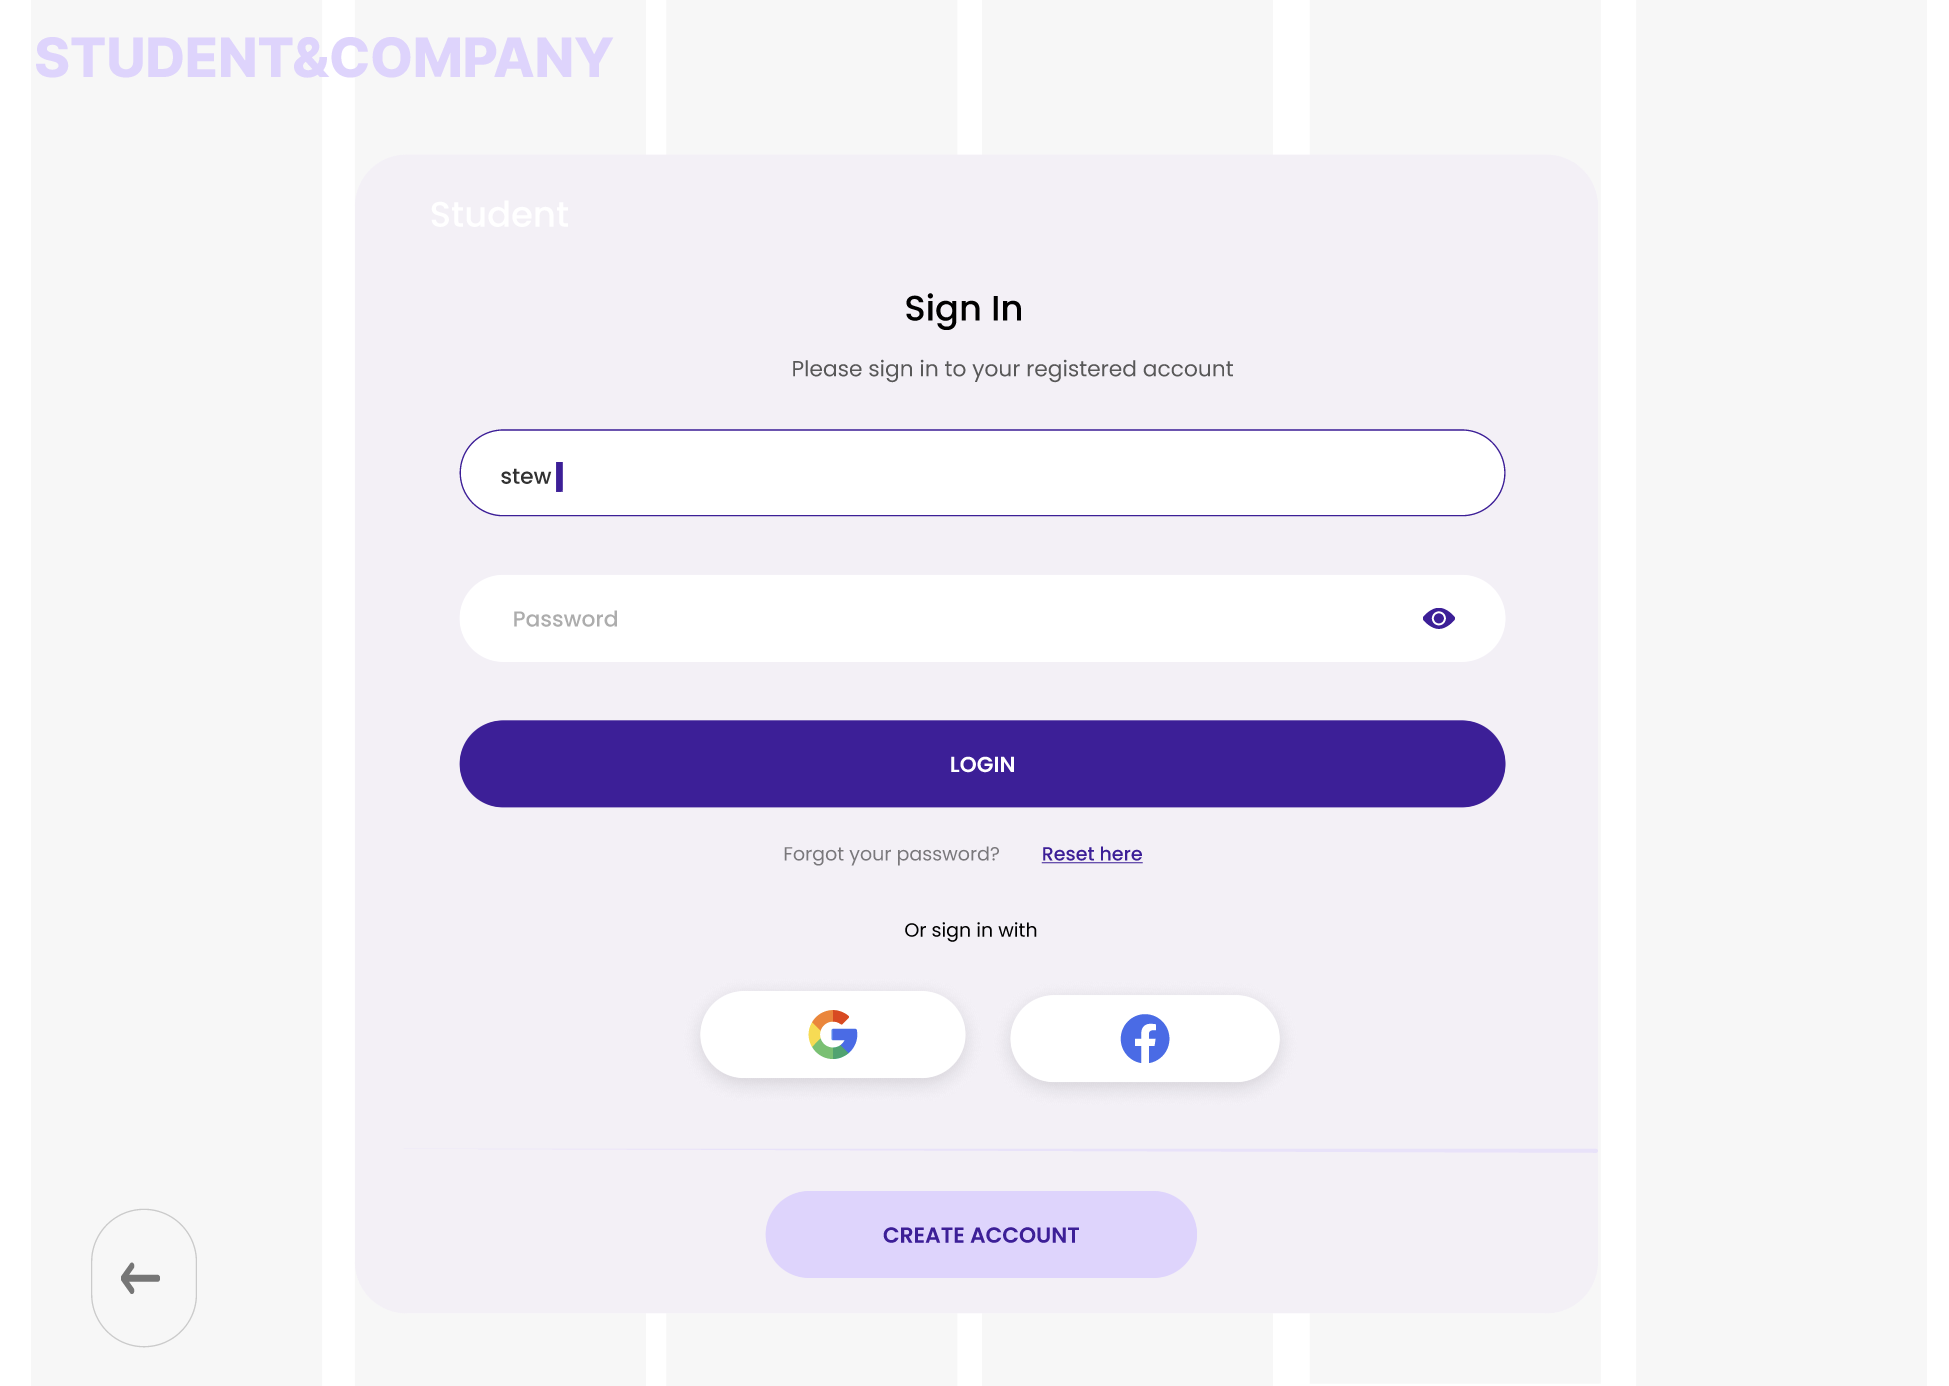
\includegraphics[width=0.5\linewidth]{Interface Images/log in sing up/Screenshot 2024-12-12 045127.png}
    \caption{Student Sign in}
    \label{fig: Student Sign in}
\end{figure}

\begin{figure} [H]
    \centering
    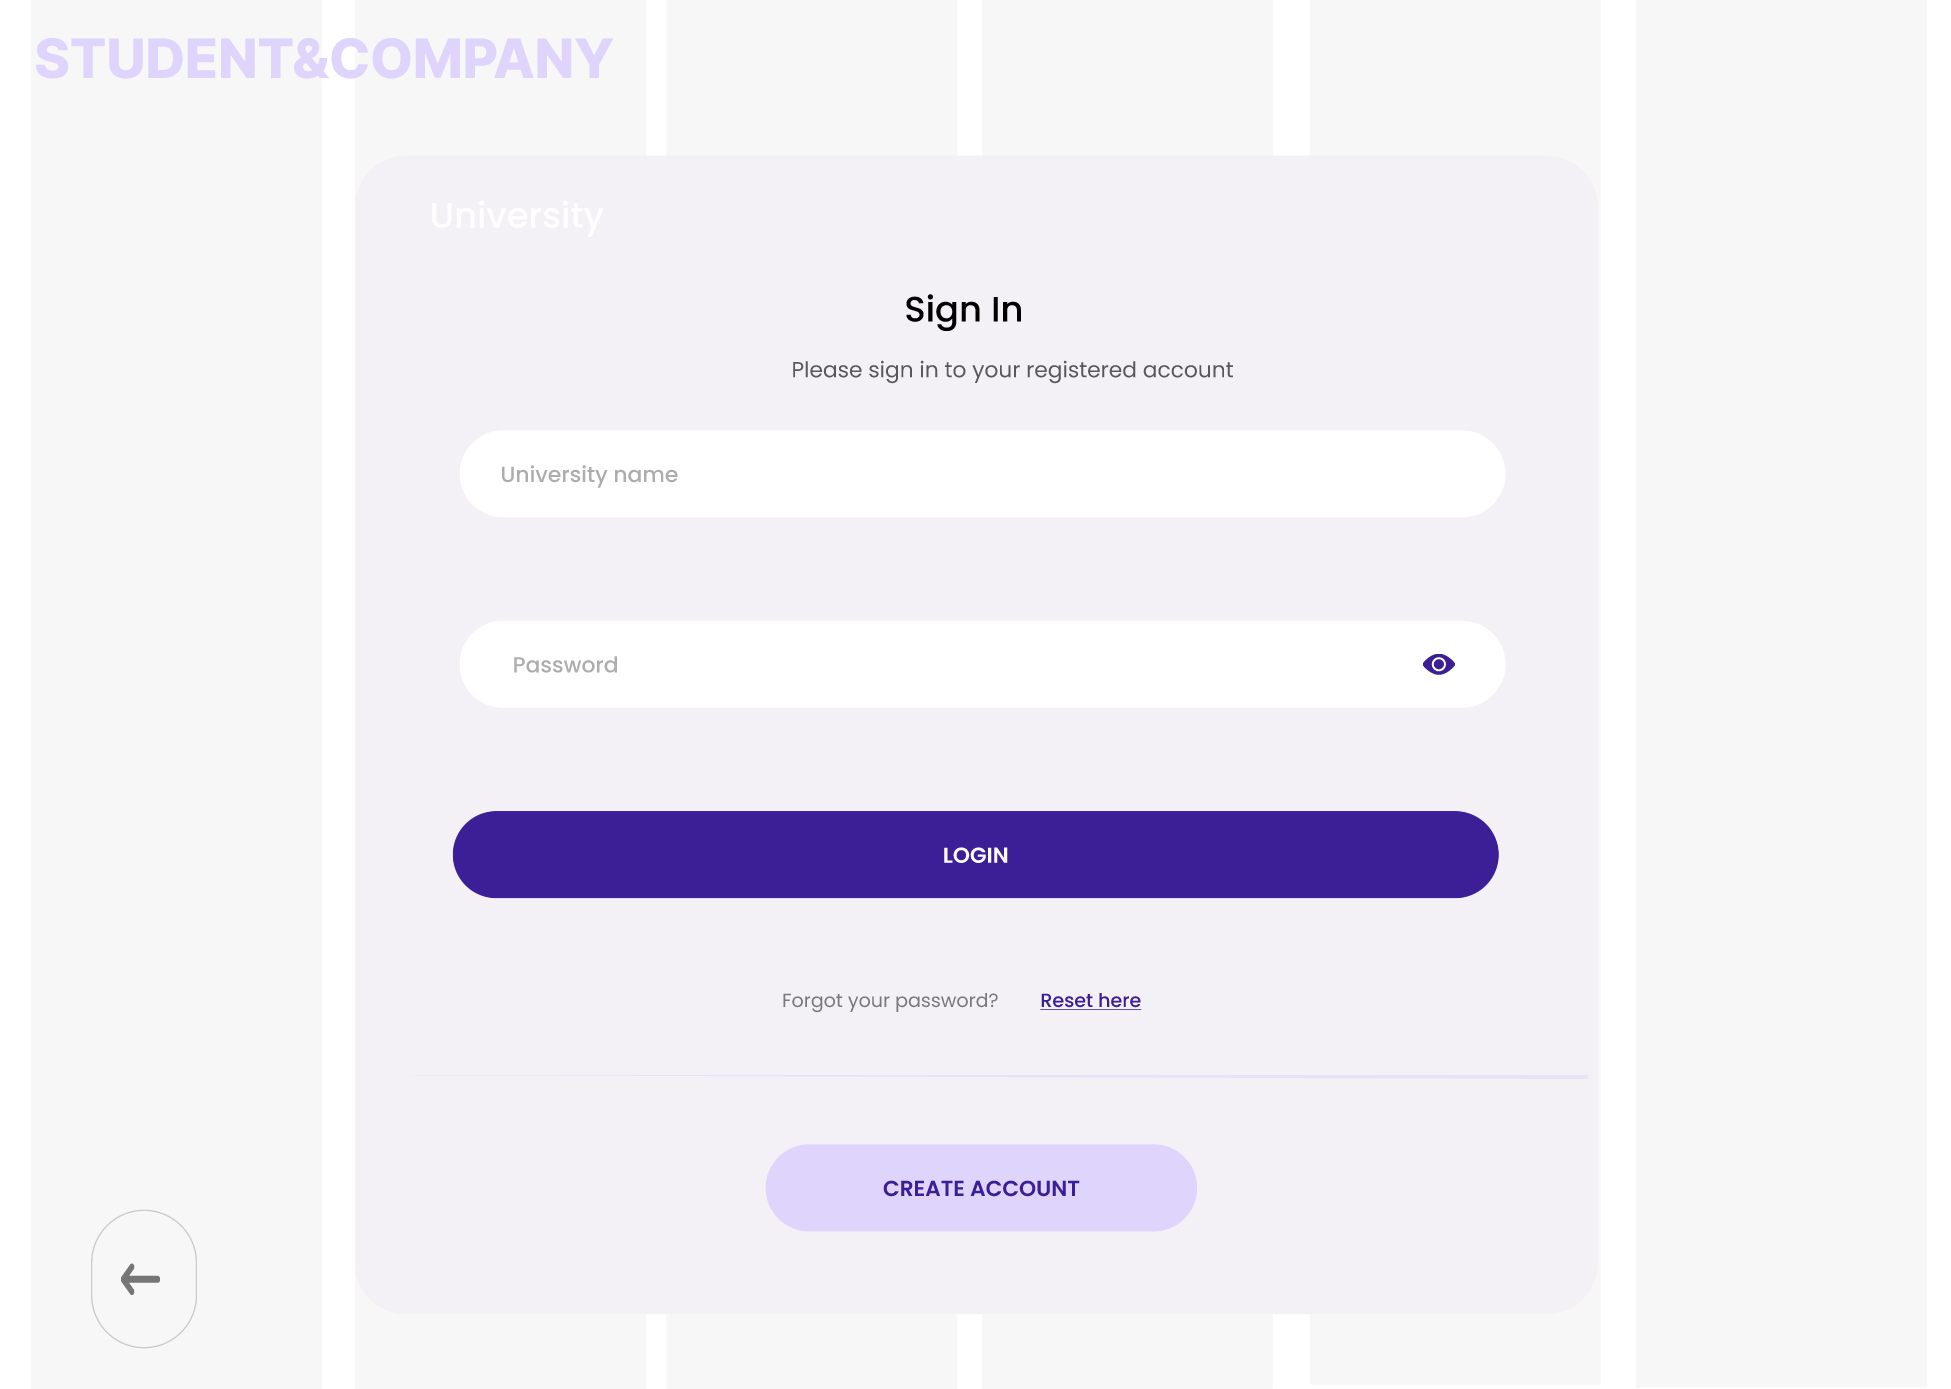
\includegraphics[width=0.5\linewidth]{Interface Images/log in sing up/Screenshot 2024-12-12 045139.png}
    \caption{University Sign in}
    \label{fig:University Sign in}
\end{figure}


\subsection{Company Interfaces}

The company's Dashboard [Figure \ref{fig:Company Home page}] serves as the central hub for all platform operations. From this main page, the company can easily access essential information, including its profile, notifications, proposed internships, and applications submitted by students. Additionally, it allows the company to communicate with students after the internship application process, as well as provide feedback or submit complaints.

\begin{figure} [H]
    \centering
    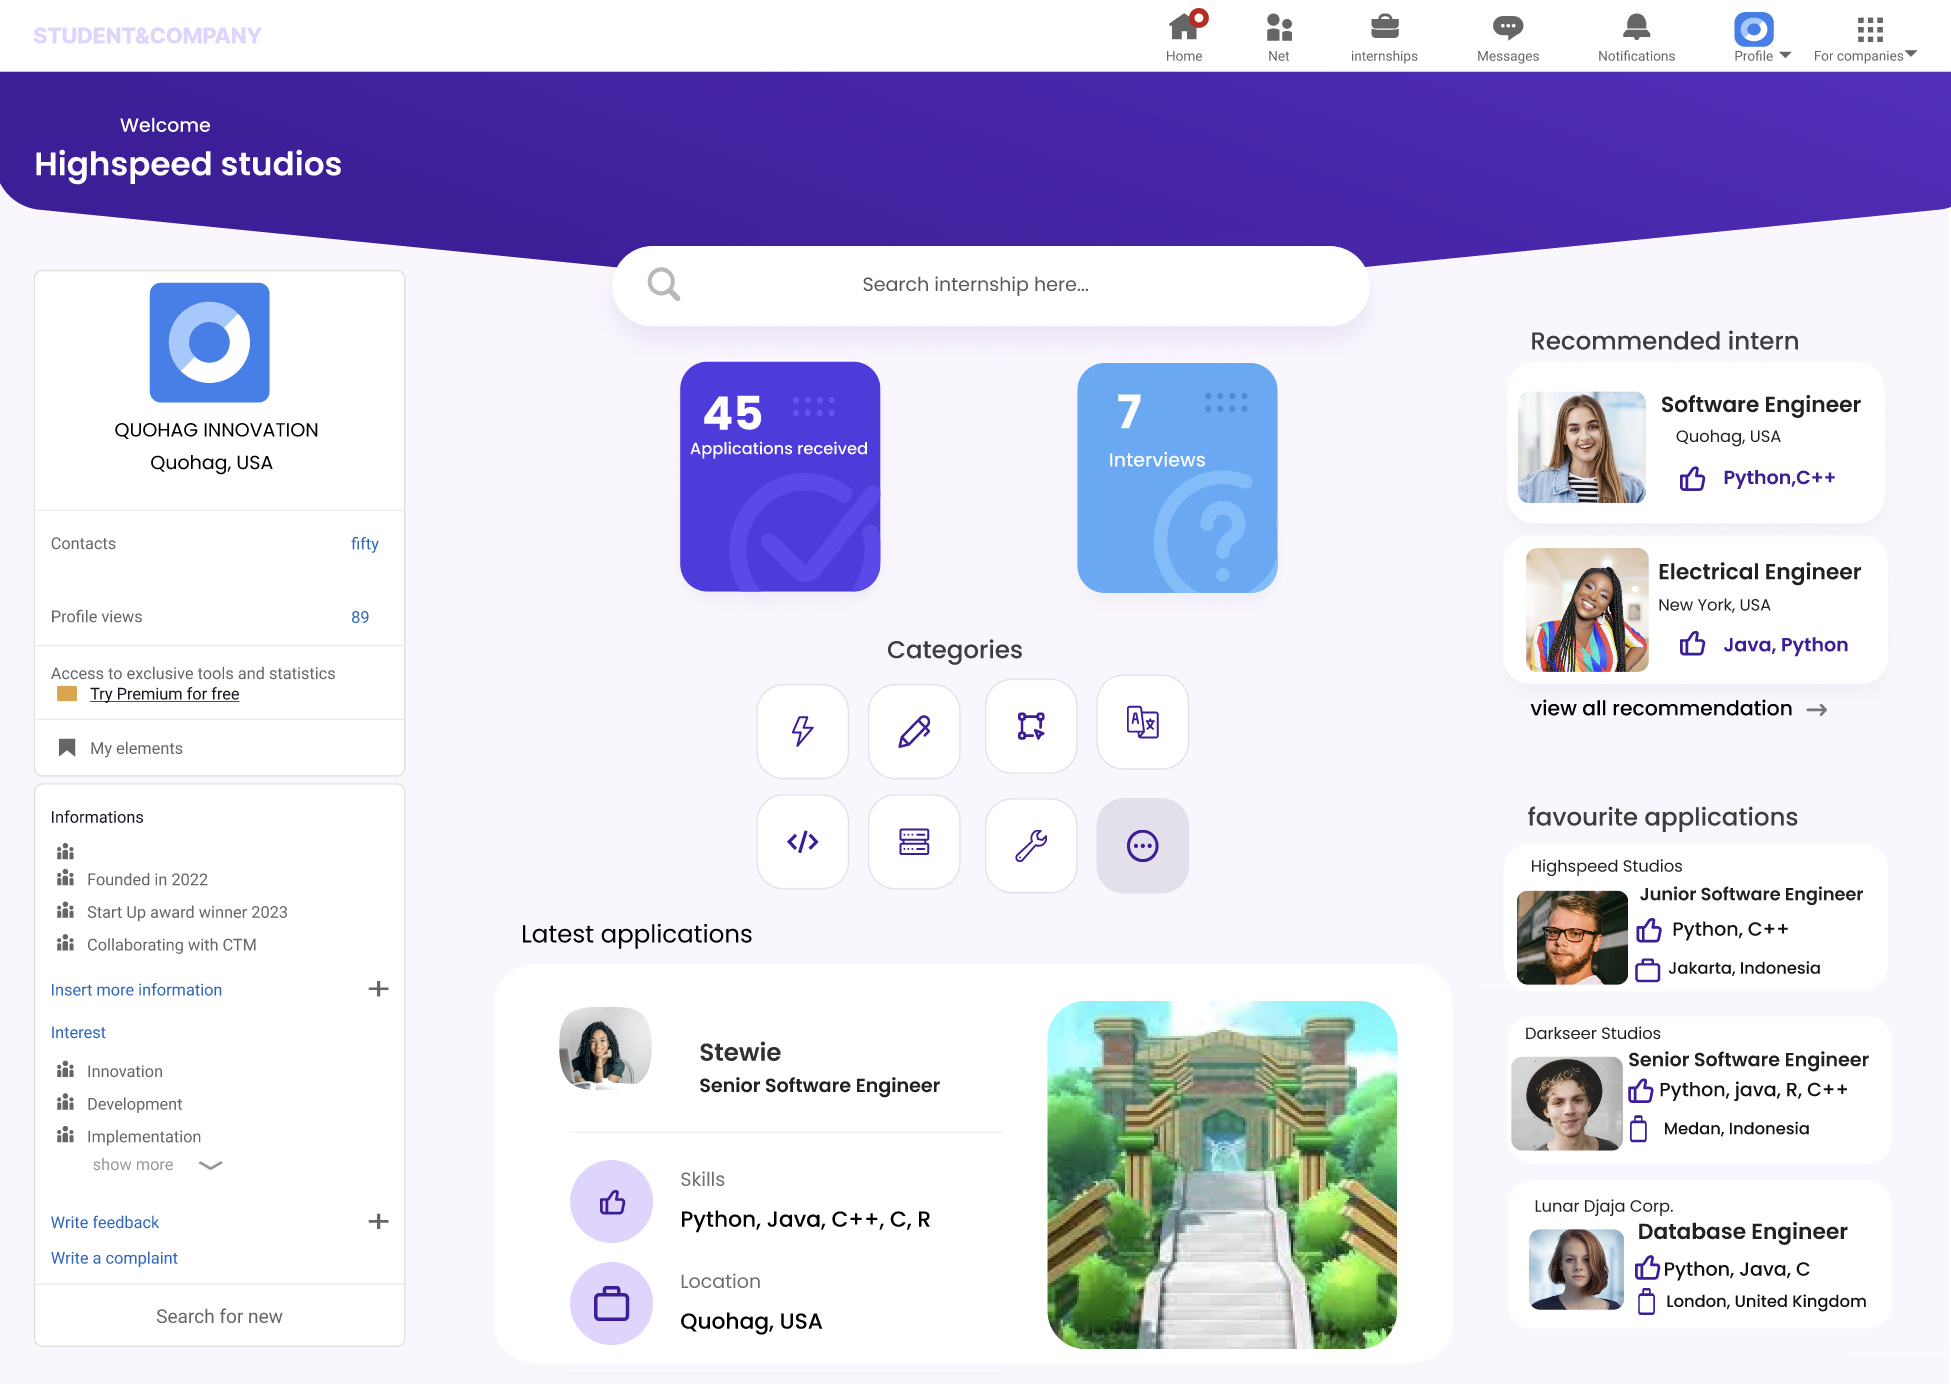
\includegraphics[width=0.5\linewidth]{Interface Images/company interface/Screenshot 2024-12-12 045319.png}
    \caption{Company Home page}
    \label{fig:Company Home page}
\end{figure}

Below, we can see the structure of a company's personal profile. It includes key details such as location, field of activity, objectives, and a dedicated section for managing internships. To edit the profile, the company simply clicks on the desired section and follows the platform's guidance. Additionally, the platform offers suggestions to enhance the provided information, making it more appealing to potential viewers[ Figures \ref{fig:Company Personal profile}, \ref{fig:Company - Managing account}].


\begin{figure} [H]
    \centering
    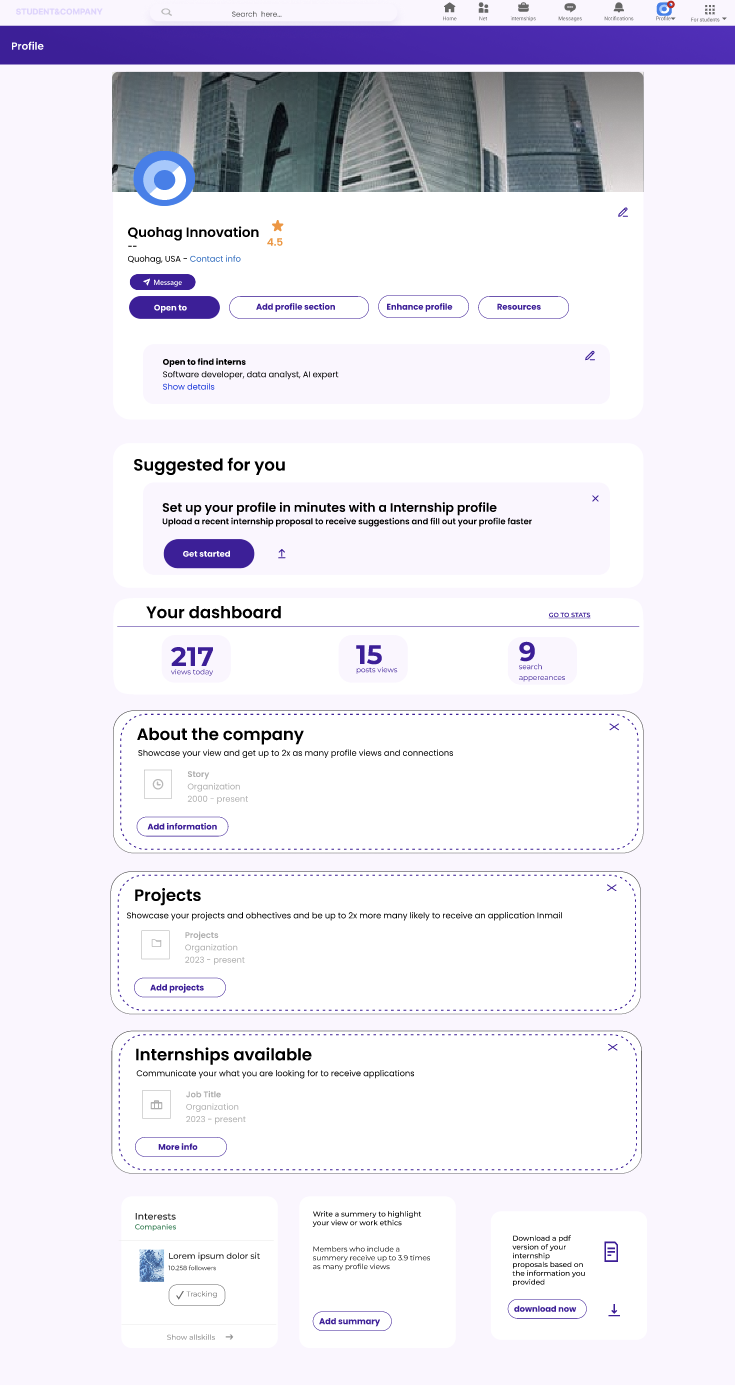
\includegraphics[width=0.5\linewidth]{Interface Images/company interface/Screenshot 2024-12-12 045502.png}
    \caption{Company Personal profile}
    \label{fig:Company Personal profile}
\end{figure}

\begin{figure} [H]
    \centering
    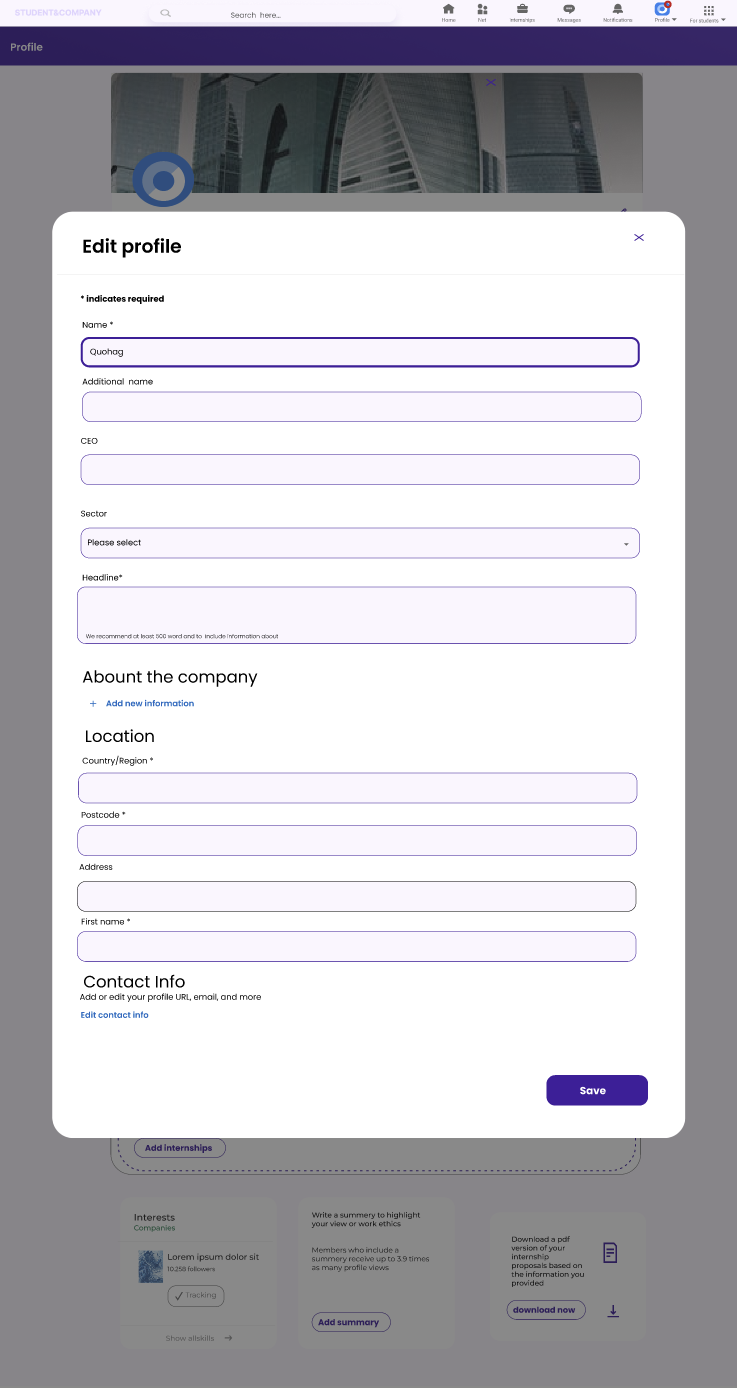
\includegraphics[width=0.5\linewidth]{Interface Images/company interface/Screenshot 2024-12-12 045535.png}
    \caption{Company - Managing account}
    \label{fig:Company - Managing account}
\end{figure}


To edit internship information, the company can click on the designated button within its personal profile. From there, it can manage the internship details while also benefiting from suggestion.s provided by the platform [Figure \ref{fig:Internships management}]. 

\begin{figure} [H]
    \centering
    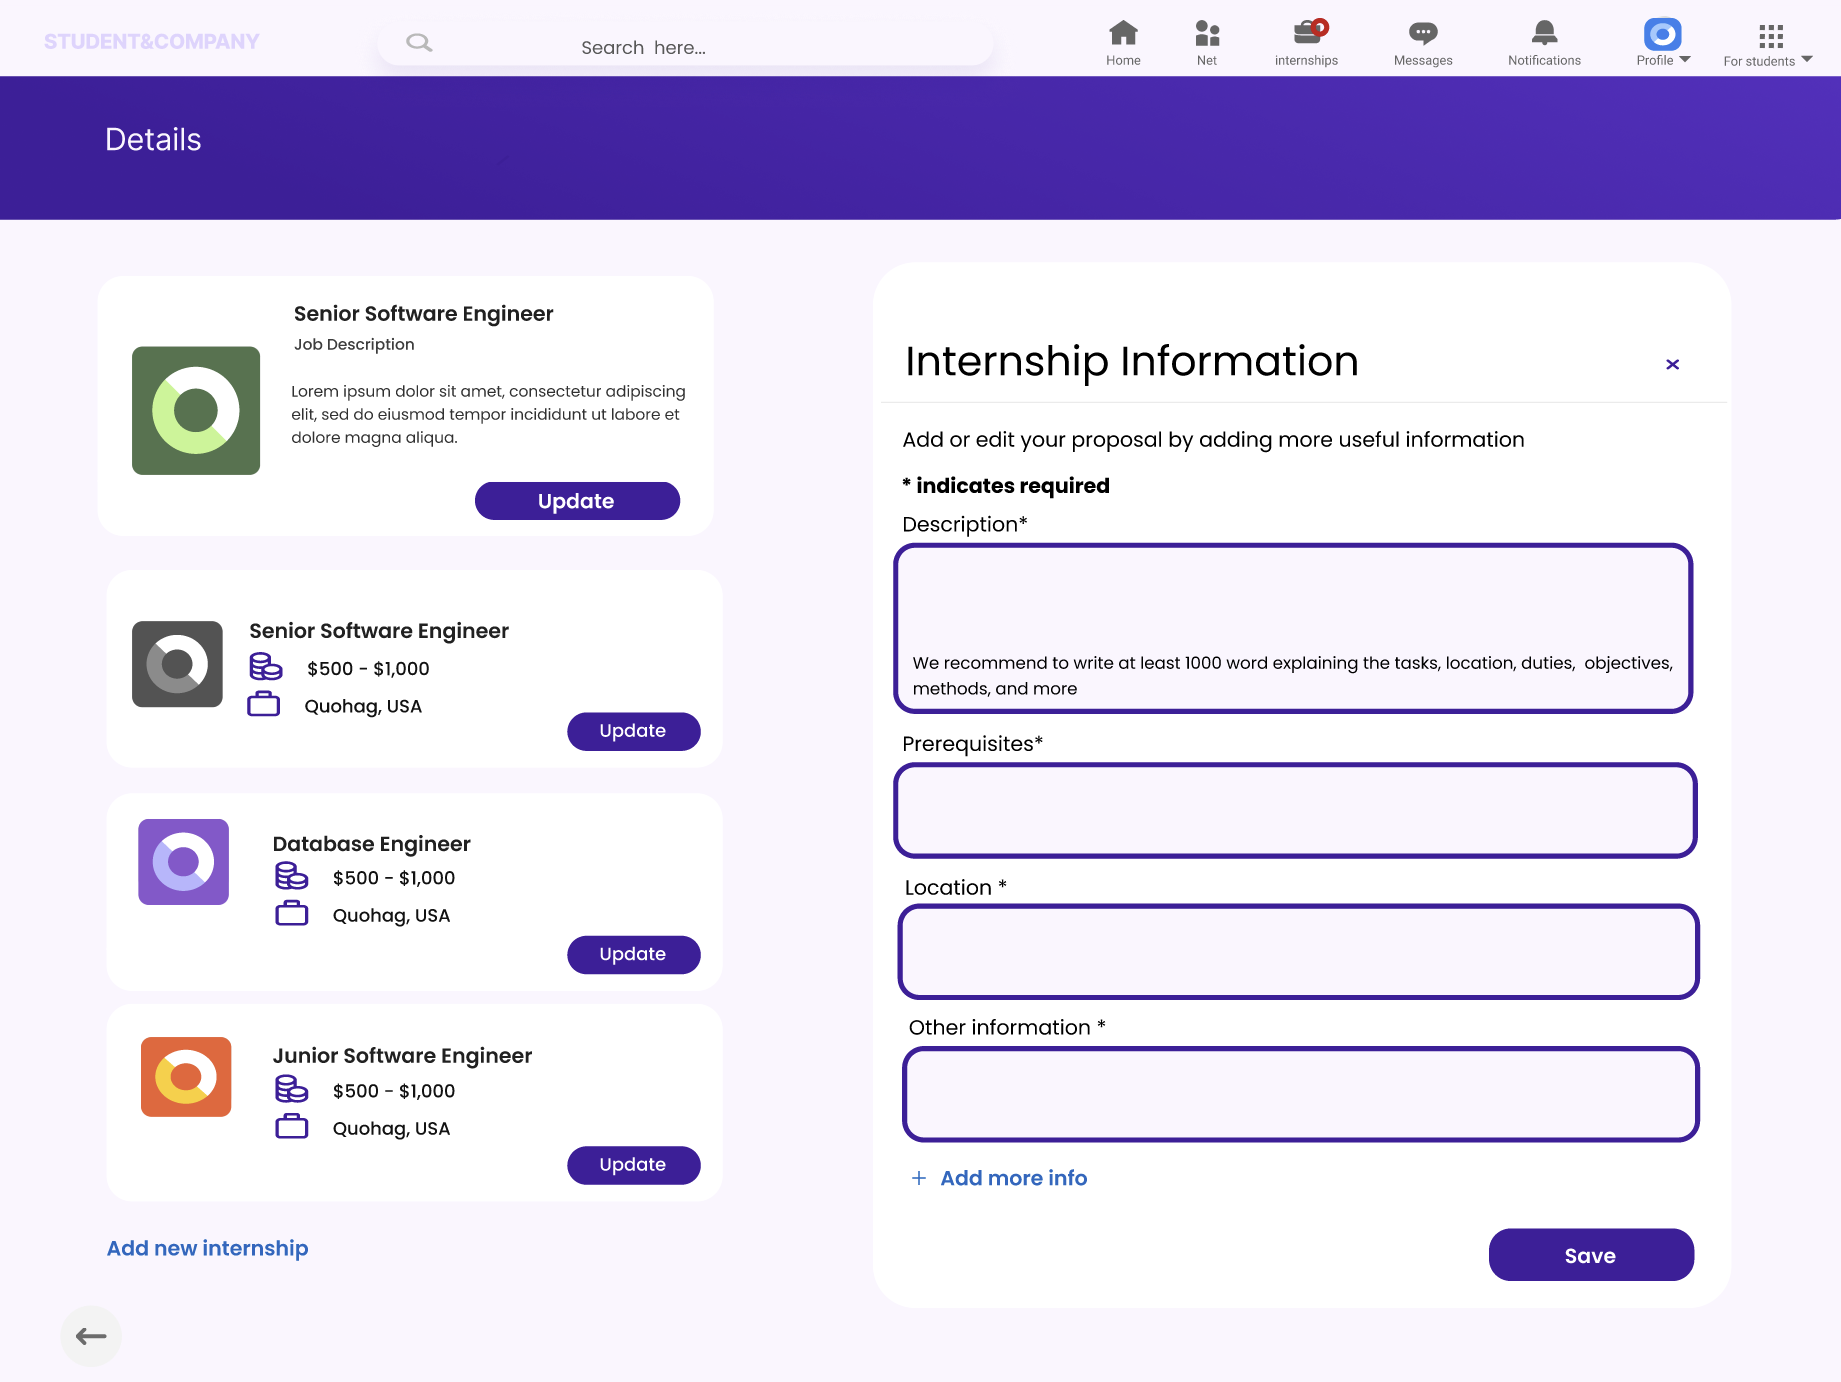
\includegraphics[width=0.5\linewidth]{Interface Images/company interface/Screenshot 2024-12-12 050044.png}
    \caption{Internships management}
    \label{fig:Internships management}
\end{figure}

On the homepage, a company can access the applications section to view all submitted applications. By selecting a specific application, the company can review its details in full, evaluate it positively or negatively, or save it for easier access later [Figure \ref{fig:Application review}] 

\begin{figure} [H]
    \centering
    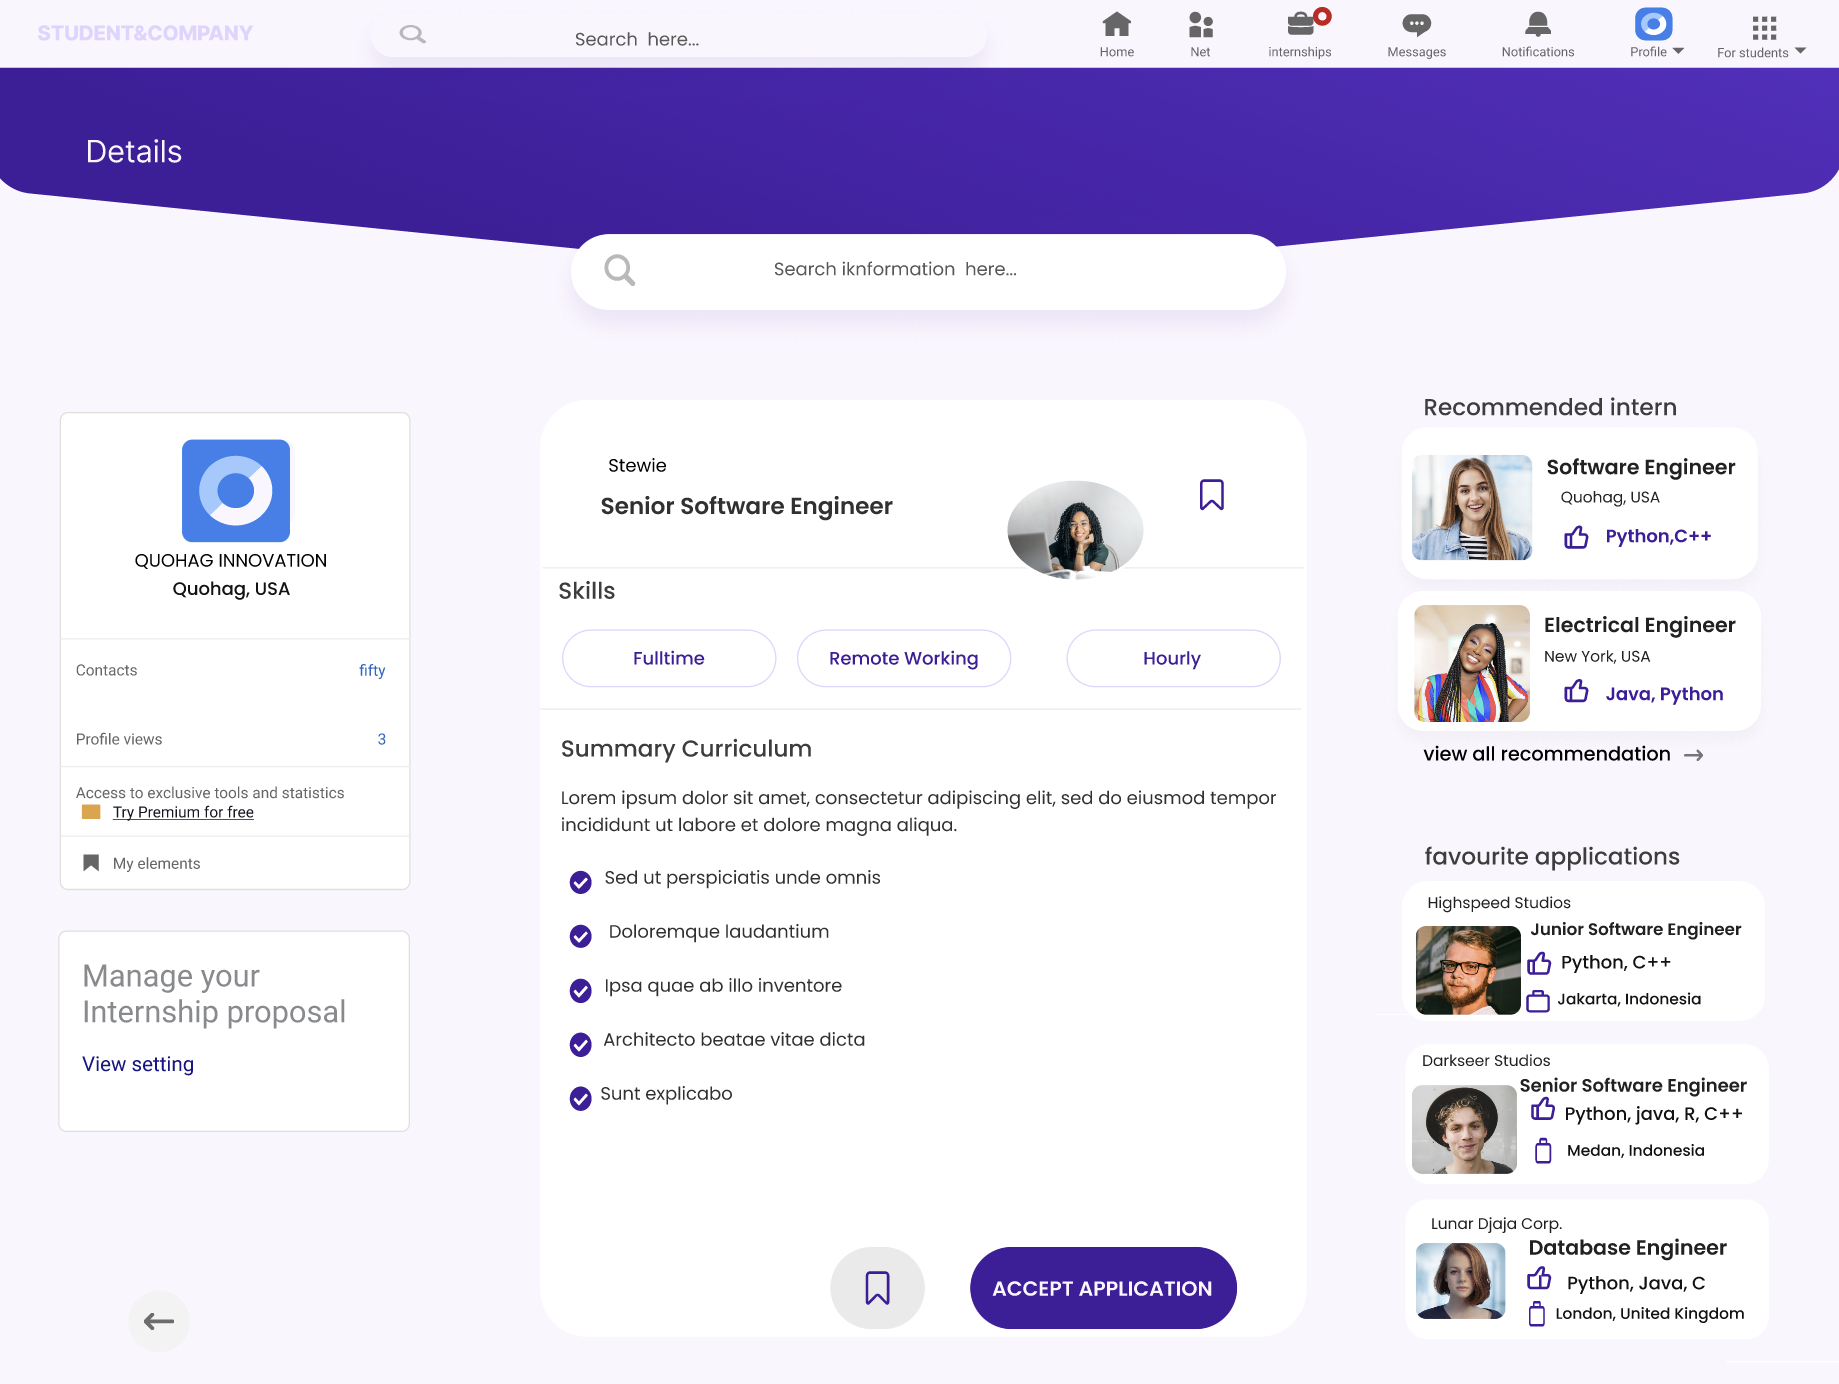
\includegraphics[width=0.5\linewidth]{Interface Images/company interface/Screenshot 2024-12-12 045731.png}
    \caption{Applications review}
    \label{fig:Application review}
\end{figure}


After positively evaluating an application, the company can interview the applicant using a structured questionnaire tailored for each internship proposal. This questionnaire is created by the company and can be enhanced with suggestions provided by the platform [Figure \ref{fig:Interview and questionnaire creation}].

\begin{figure} [H]
    \centering
    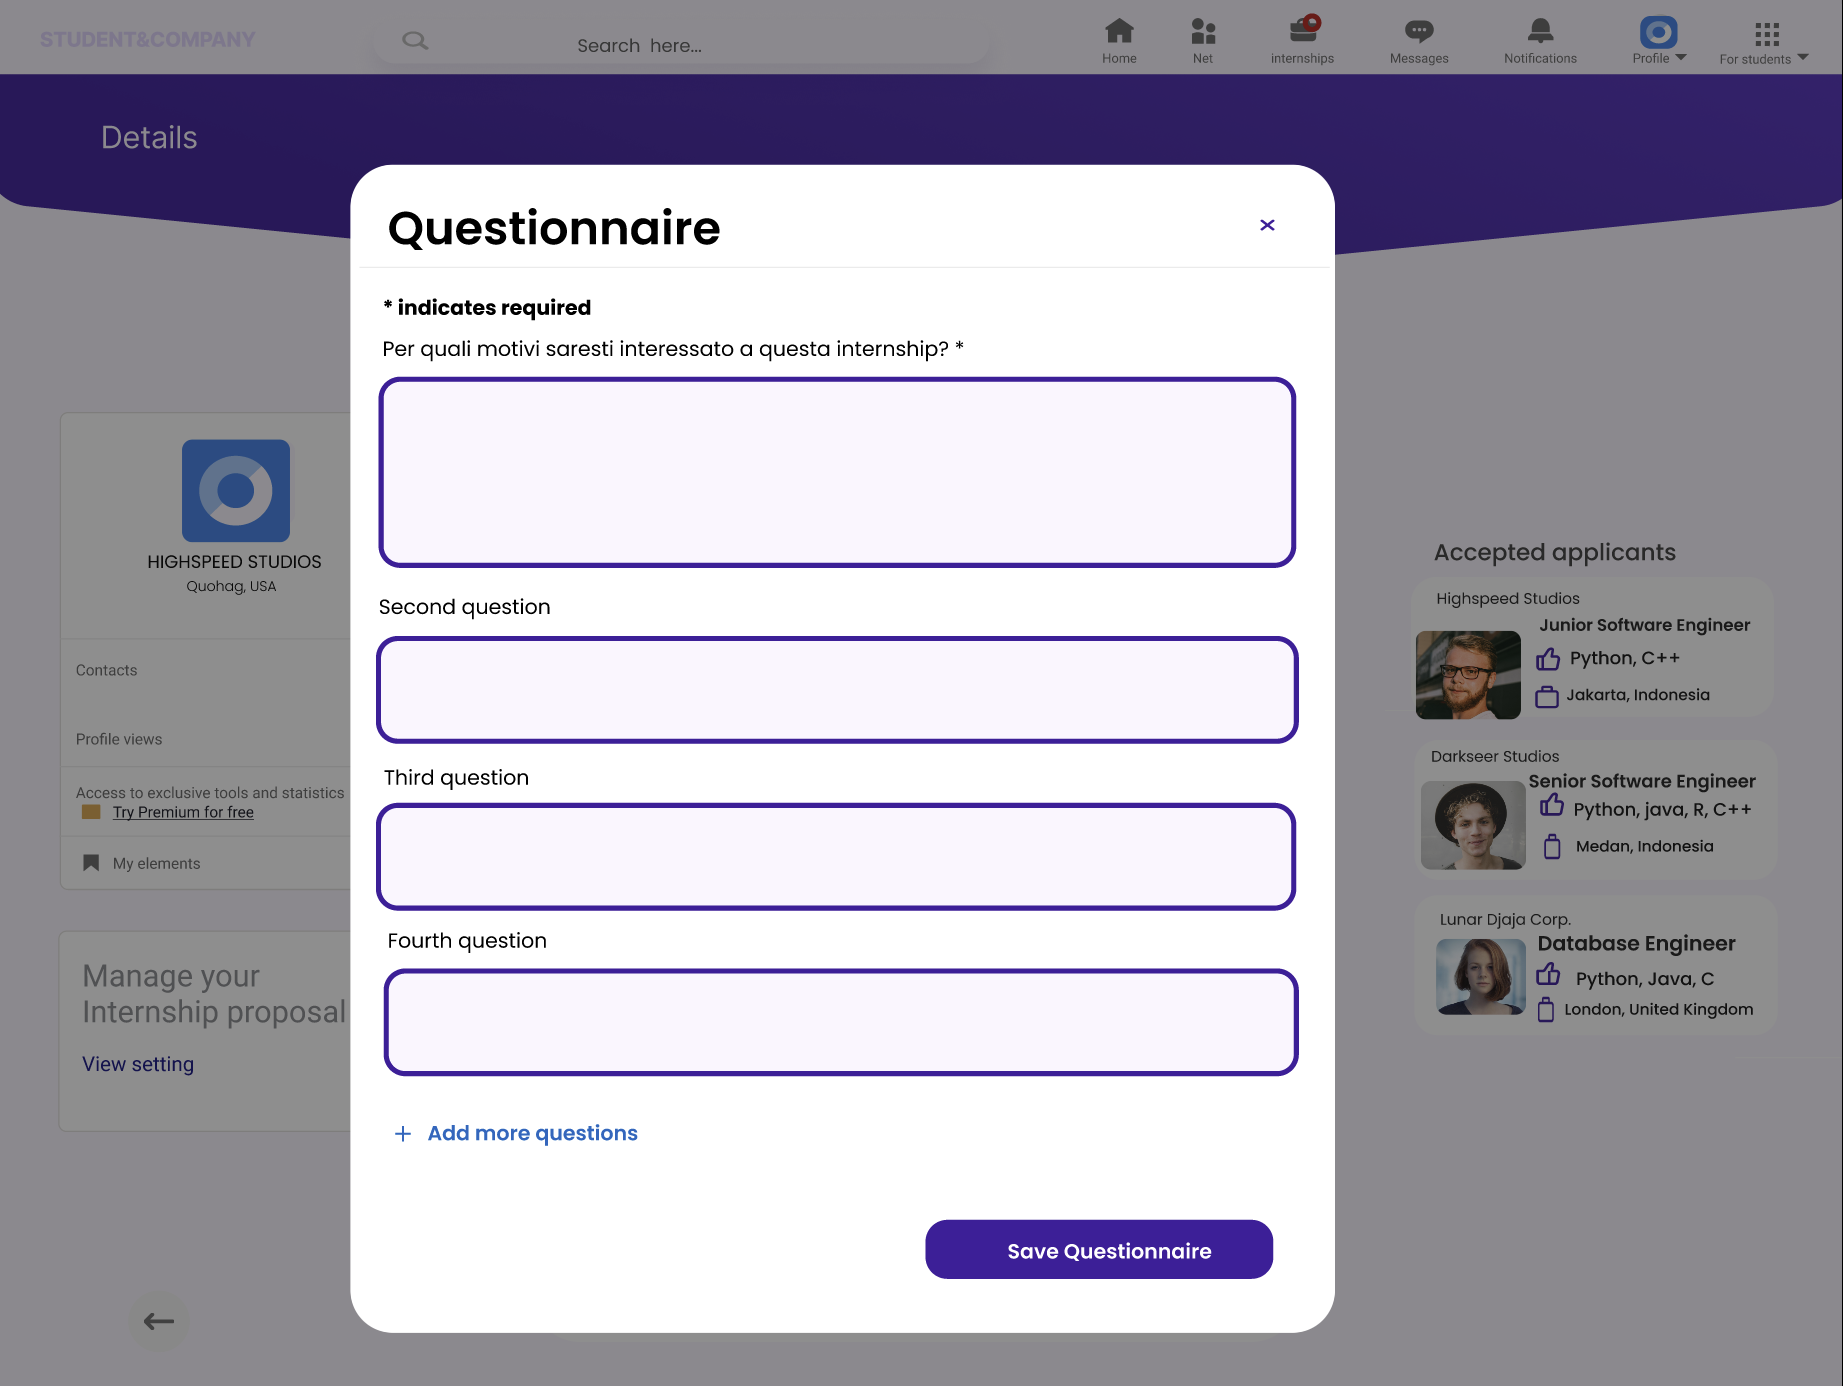
\includegraphics[width=0.5\linewidth]{Interface Images/company interface/Screenshot 2024-12-12 045749.png}
    \caption{Interview and questionnaire creation}
    \label{fig:Interview and questionnaire creation}
\end{figure}

Once a student has completed the questionnaire, the company reviews the submitted answers and evaluates the application. The company can either decline it by providing a negative evaluation or accept it, officially initiating the internship [Figure \ref{fig:Interviews evaluation}].

\begin{figure} [H]
    \centering
    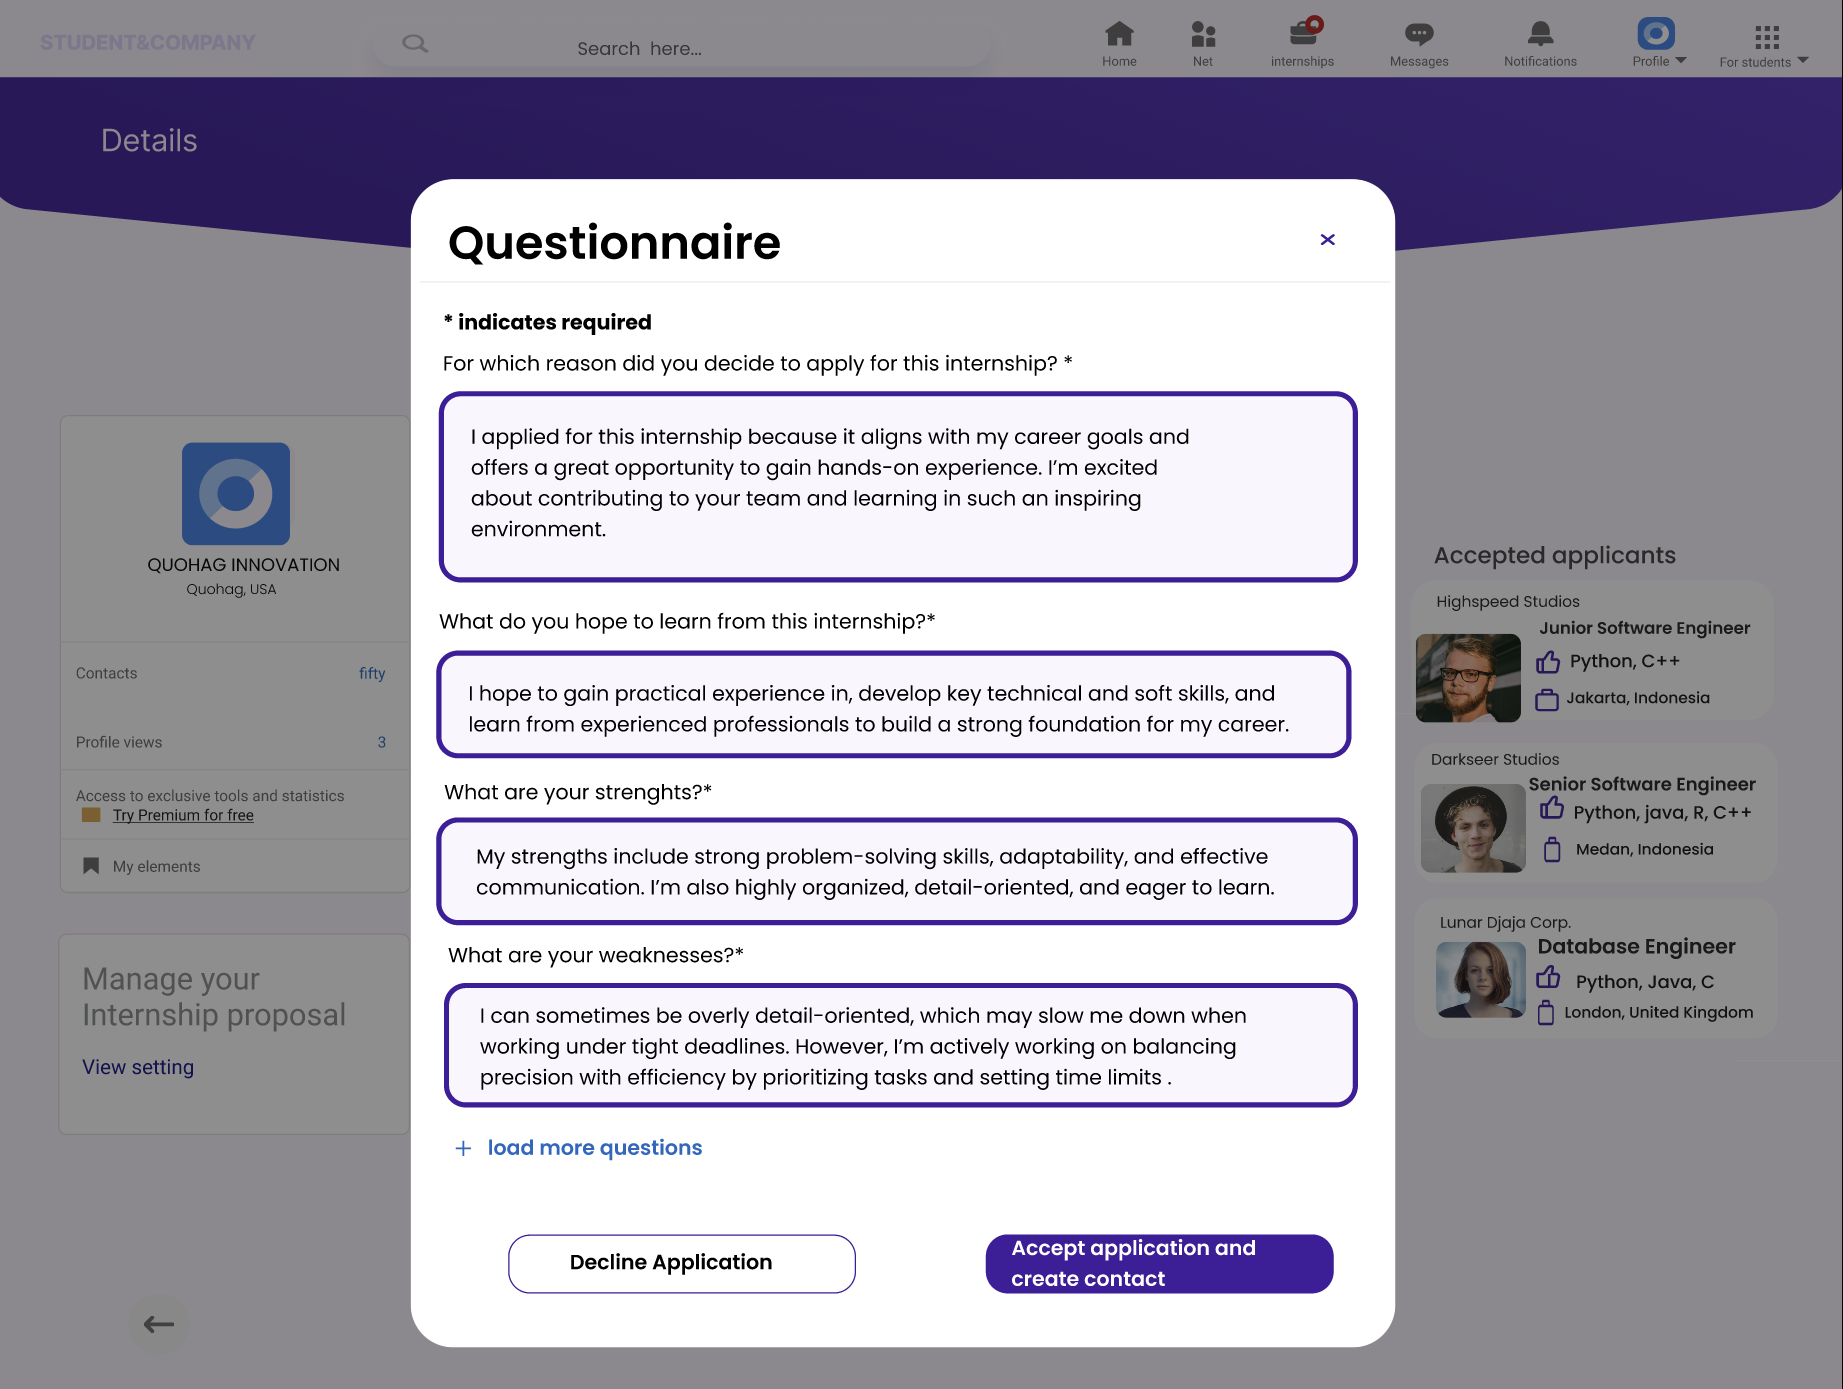
\includegraphics[width=0.5\linewidth]{Interface Images/company interface/Screenshot 2024-12-12 045902.png}
    \caption{Interview evaluation}
    \label{fig:Interviews evaluation}
\end{figure}


\subsection{Student Interfaces}

The student dashboard [Figure \ref{fig:Student Home page}] is the centre of all possible operations on the platform. From this main page, the student can have access to all essential information,
including their personal profile, notifications, available internships, and applications submitted to companies. In addition, it allows the student to communicate with the company after the internship application process is over, as well as provide feedback or submit complaints.

\begin{figure} [H]
    \centering
    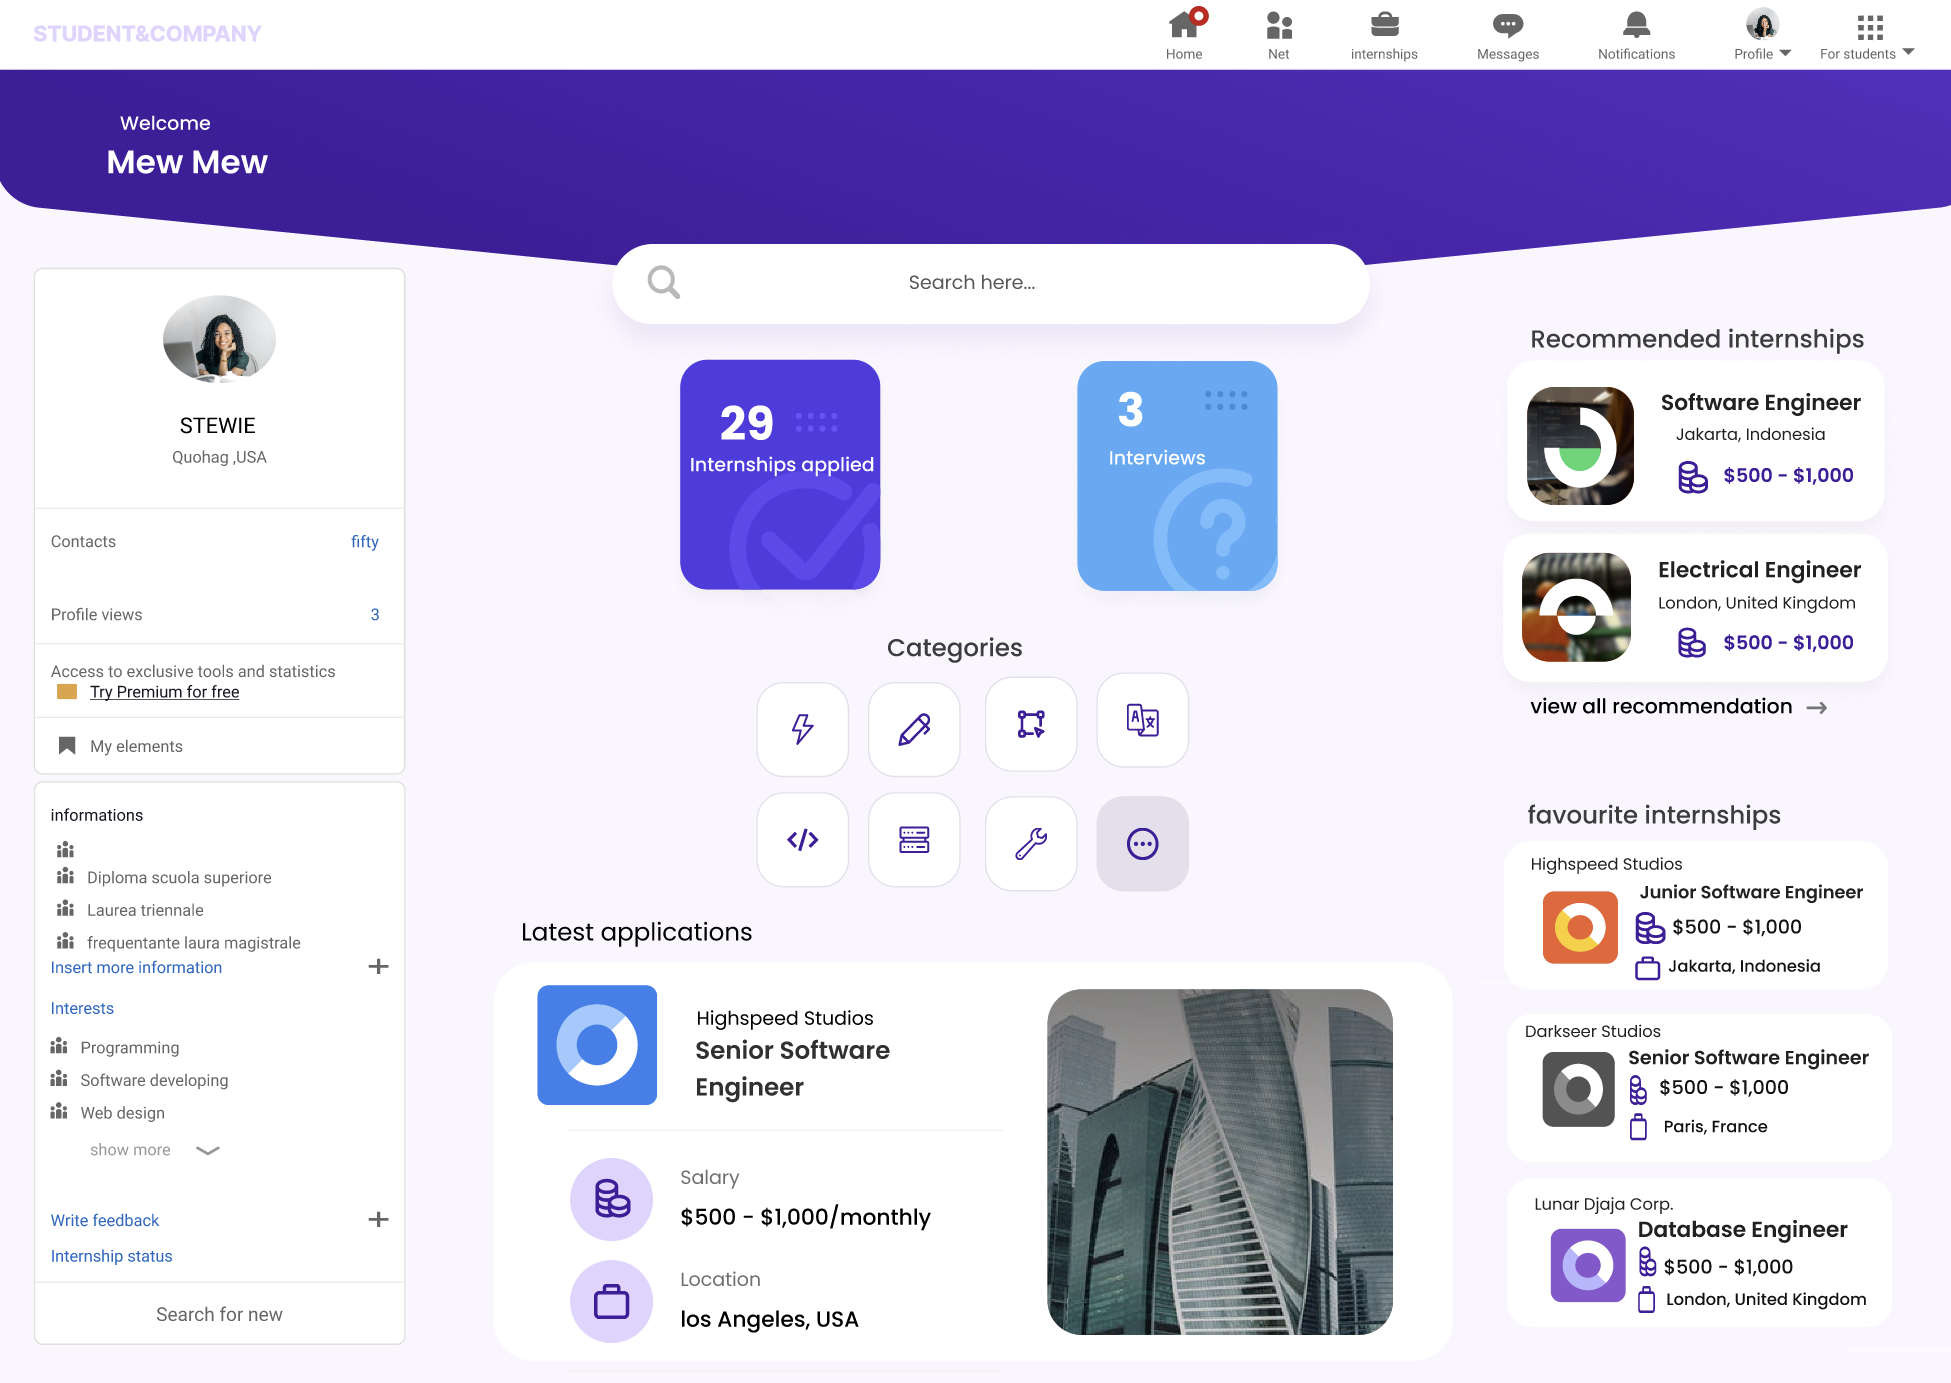
\includegraphics[width=0.5\linewidth]{Interface Images/student interface/Screenshot 2024-12-12 045307.png}
    \caption{Student Home page}
    \label{fig:Student Home page}
\end{figure}

In the personal profile section, students can input their personal details as well as information relevant to creating a CV for internship applications. Students have the option to enter this information independently or follow platform suggestions and tips to enhance their CV, making it more appealing to potential employers. The information is organized into sections and will be visible to companies later on.

\begin{figure} [H]
    \centering
    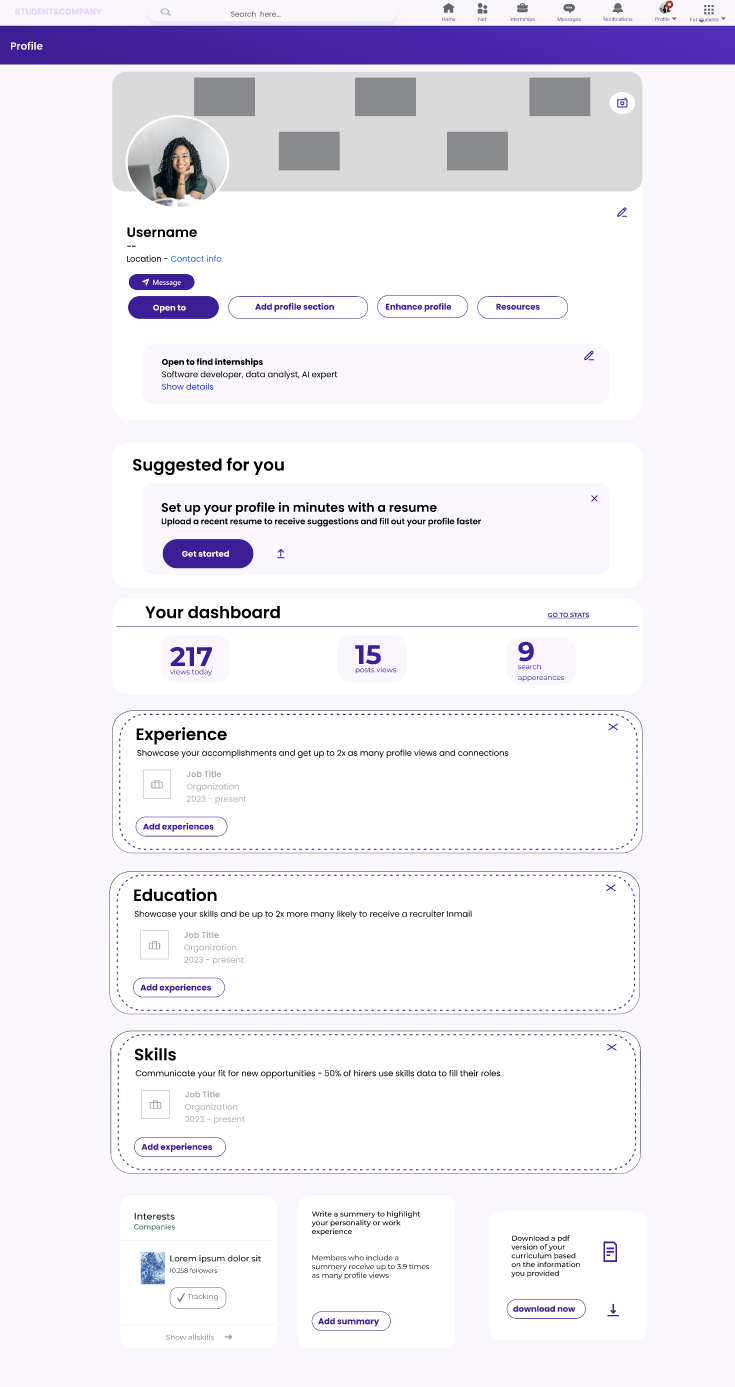
\includegraphics[width=0.5\linewidth]{Interface Images/student interface/Screenshot 2024-12-12 045421.png}
    \caption{Student Personal profile}
    \label{fig:Student Personal profile}
\end{figure}

\begin{figure} [H]
    \centering
    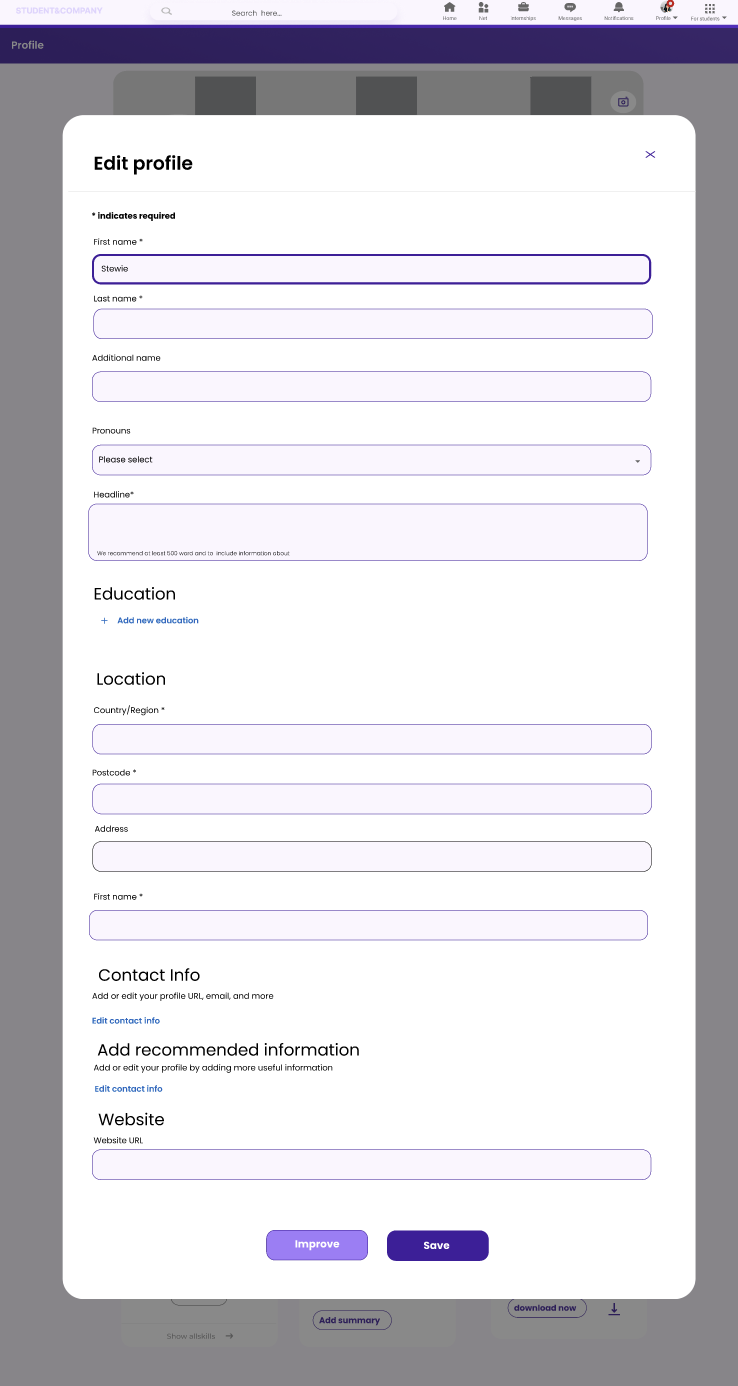
\includegraphics[width=0.5\linewidth]{Interface Images/student interface/Screenshot 2024-12-12 045447.png}
    \caption{Student Profile management}
    \label{fig:Student Profile management}
\end{figure}


In the search section, students can explore all available internships on the platform. To make the search more relevant and tailored to their personal interests, several filters are provided, allowing students to select internships based on criteria they specify. The internships will be displayed in a list, showing only key details. By clicking on a specific internship, students can view all the information and find the option to apply if they're interested in that particular opportunity.

\begin{figure} [H]
    \centering
    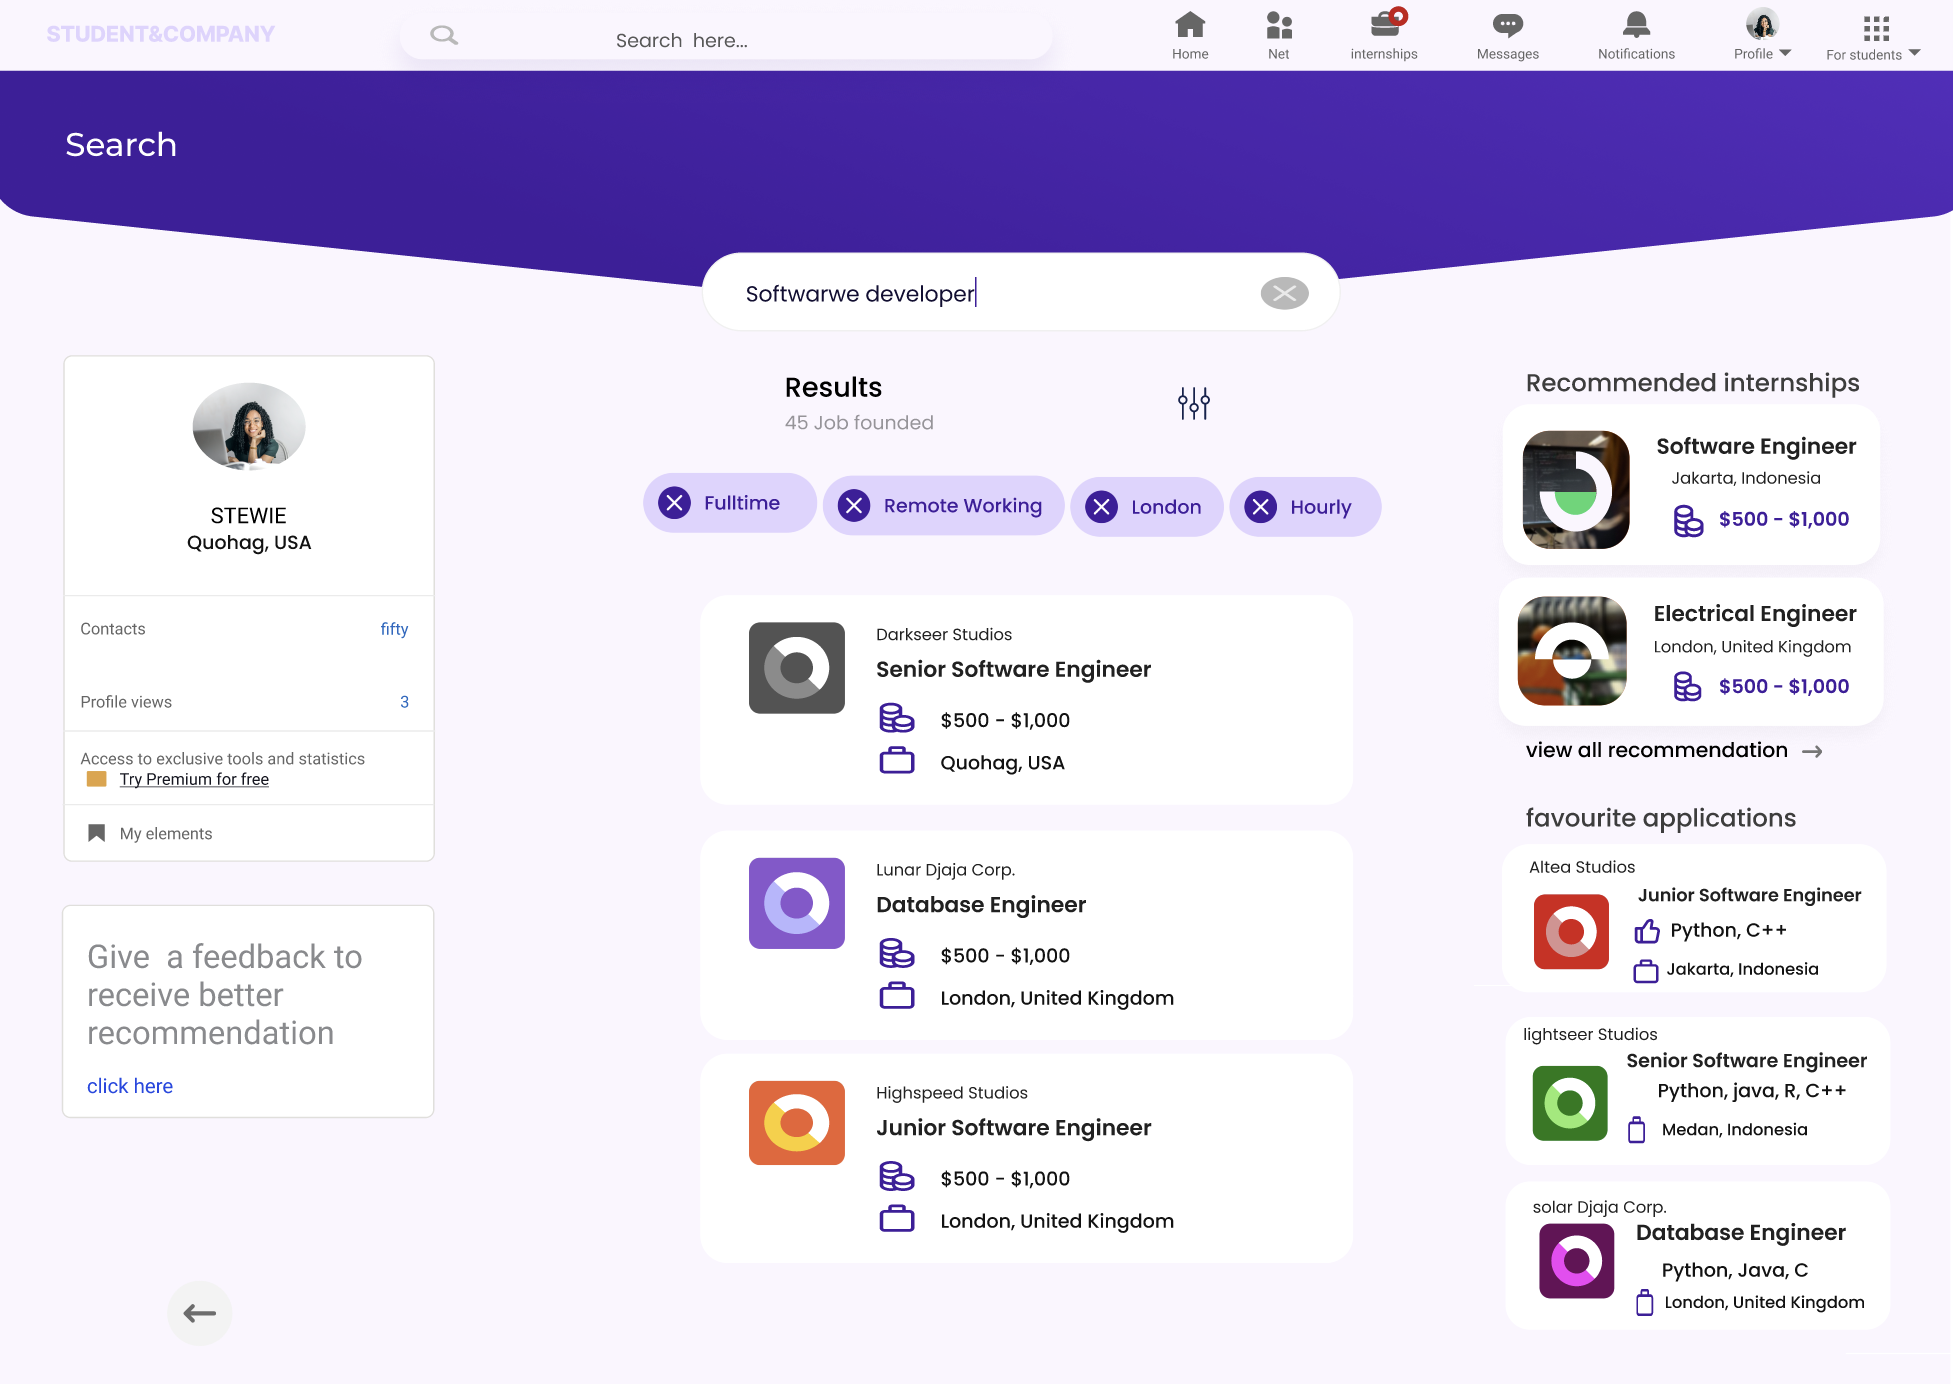
\includegraphics[width=0.5\linewidth]{Interface Images/student interface/Screenshot 2024-12-12 045606.png}
    \caption{Internships lookup}
    \label{fig: Internships lookup}
\end{figure}

\begin{figure} [H]
    \centering
    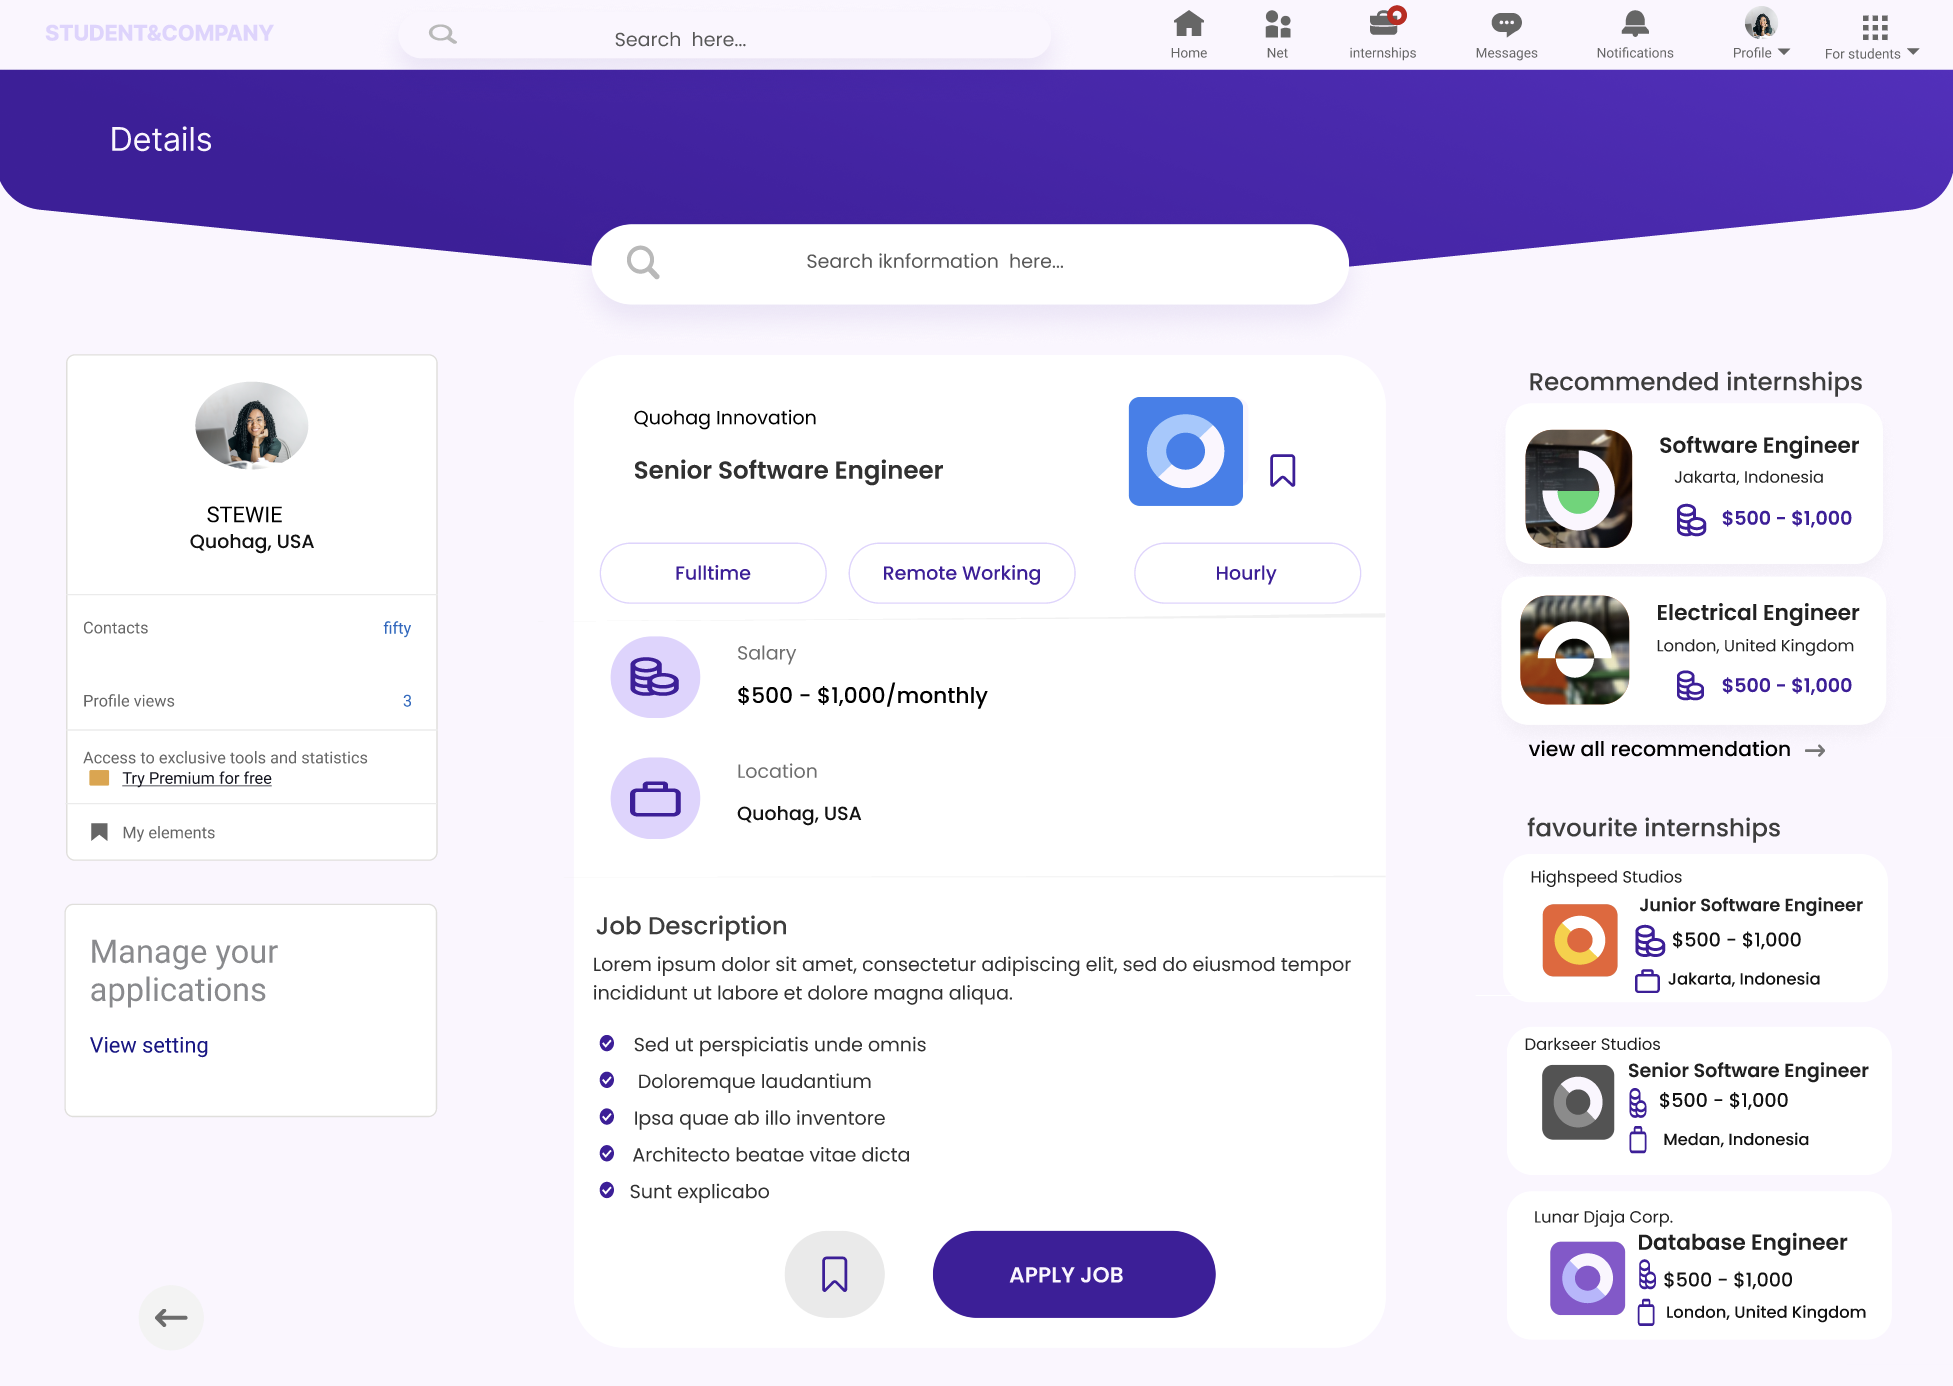
\includegraphics[width=0.5\linewidth]{Interface Images/student interface/Screenshot 2024-12-12 045619.png}
    \caption{Internship details}
    \label{fig:Internship details}
\end{figure}

After clicking the "Apply" button, the student can proceed with the internship application. To complete the application, the student must either upload their CV or consent to share their personal profile information with the company. Additionally, the student will need to provide other personal details, such as their name, surname, and email. Once all the required information is submitted, the student can send the application.

\begin{figure} [H]
    \centering
    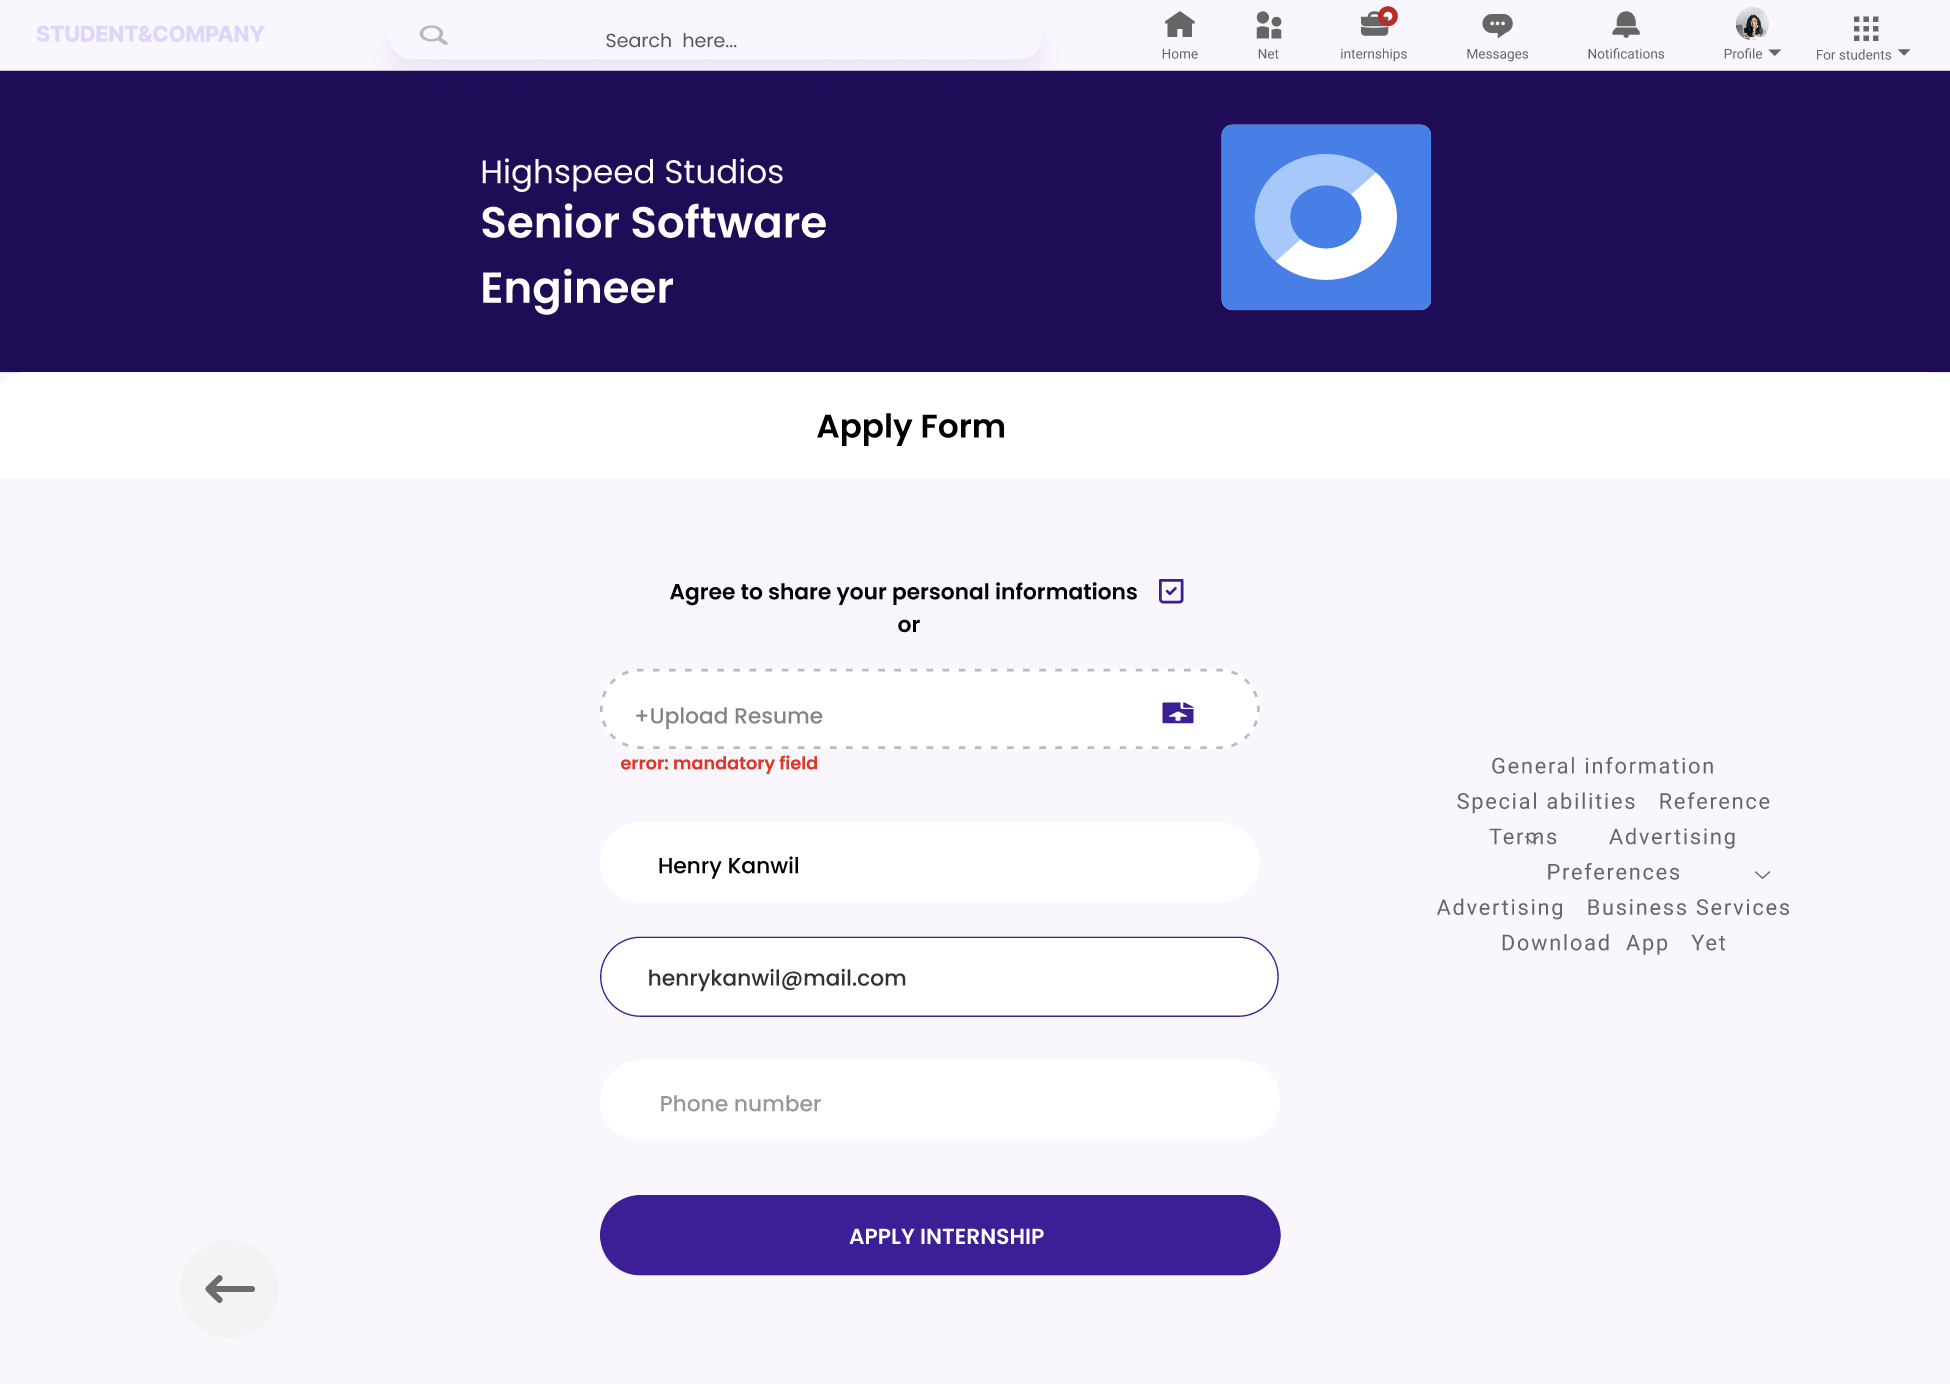
\includegraphics[width=0.5\linewidth]{Interface Images/student interface/Screenshot 2024-12-12 045639.png}
    \caption{Application form}
    \label{fig:Application form}
\end{figure}

Once an application is submitted and a positive evaluation is received, the interview section will become available on the internship page. The interview is structured as a questionnaire, which is pre-prepared by the company for each specific internship. The student must answer all questions in the questionnaire before submitting it back to the company for final evaluation. Based on this evaluation, the company will make the final decision on whether to proceed with the internship.


\begin{figure} [H]
    \centering
    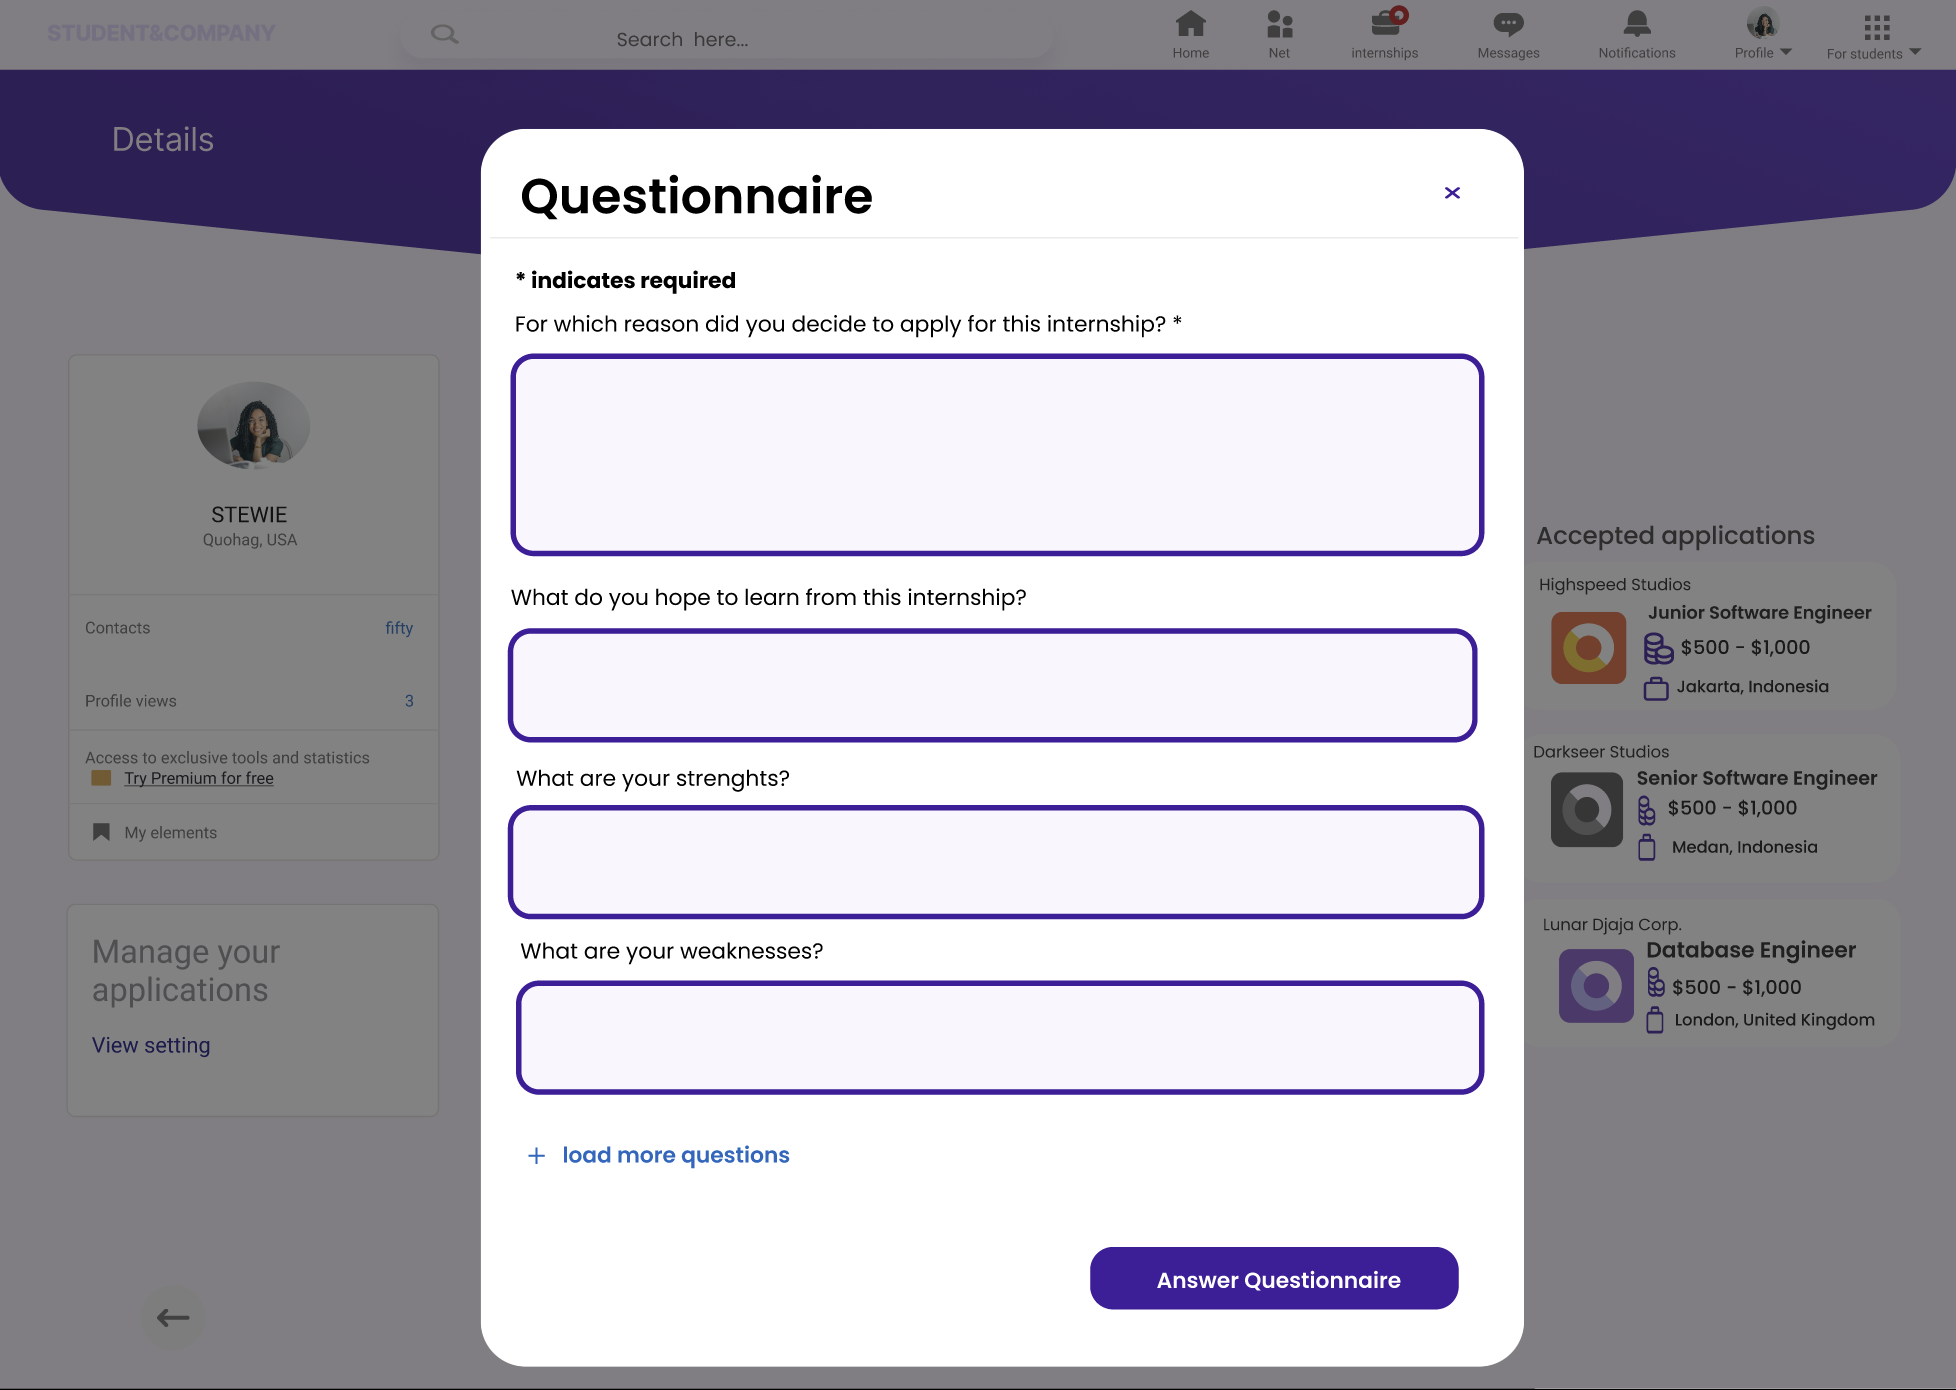
\includegraphics[width=0.5\linewidth]{Interface Images/student interface/Screenshot 2024-12-12 045852.png}
    \caption{Interview reply}
    \label{fig:Interview reply}
\end{figure}

Throughout the application process, the student will be able to monitor the status of their application and receive notifications whenever there is a change. The status will update based on different stages, including: application sent, awaiting review, evaluated negatively, evaluated positively, interview ready, interview submitted, and interview evaluated.

\begin{figure} [H]
    \centering
    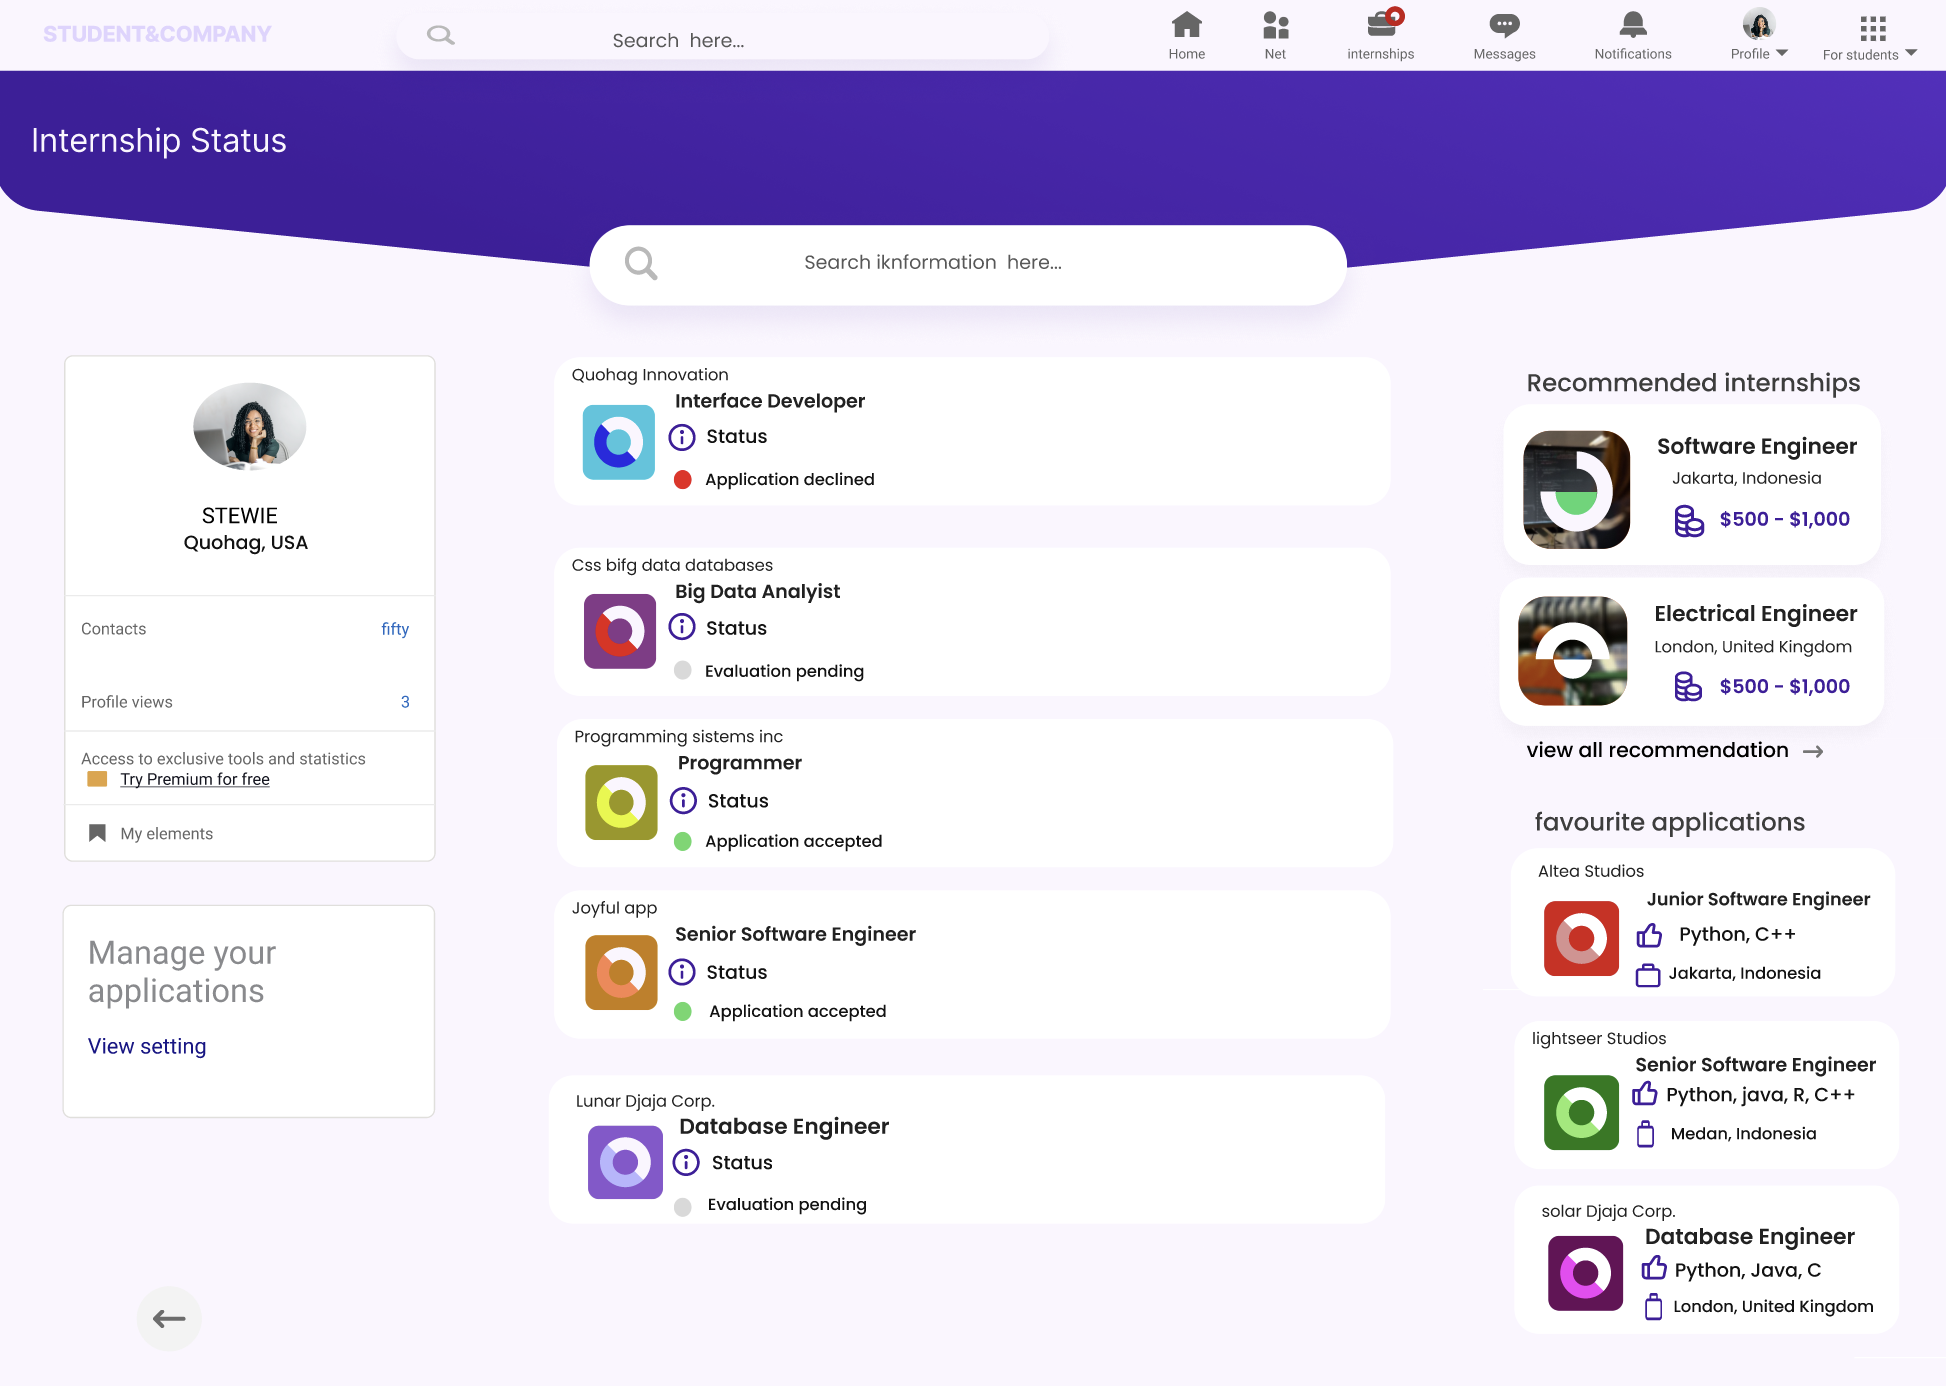
\includegraphics[width=0.5\linewidth]{Interface Images/student interface/Screenshot 2024-12-12 050031.png}
    \caption{Application status}
    \label{fig:Application status}
\end{figure}

\subsection{University Interfaces}


The university's Dashboard [Figure \ref{fig: University Home page}] serves as the central hub for all platform operations. From this main page, the university can easily access essential information, including its notifications the personal profiles of the students enrolled, and all complaints sent by both students and companies. Additionally, it allows the university to communicate with students and companies after a complaint has been submitted, allowing for a better resolution of the problems.

\begin{figure} [H]
    \centering
    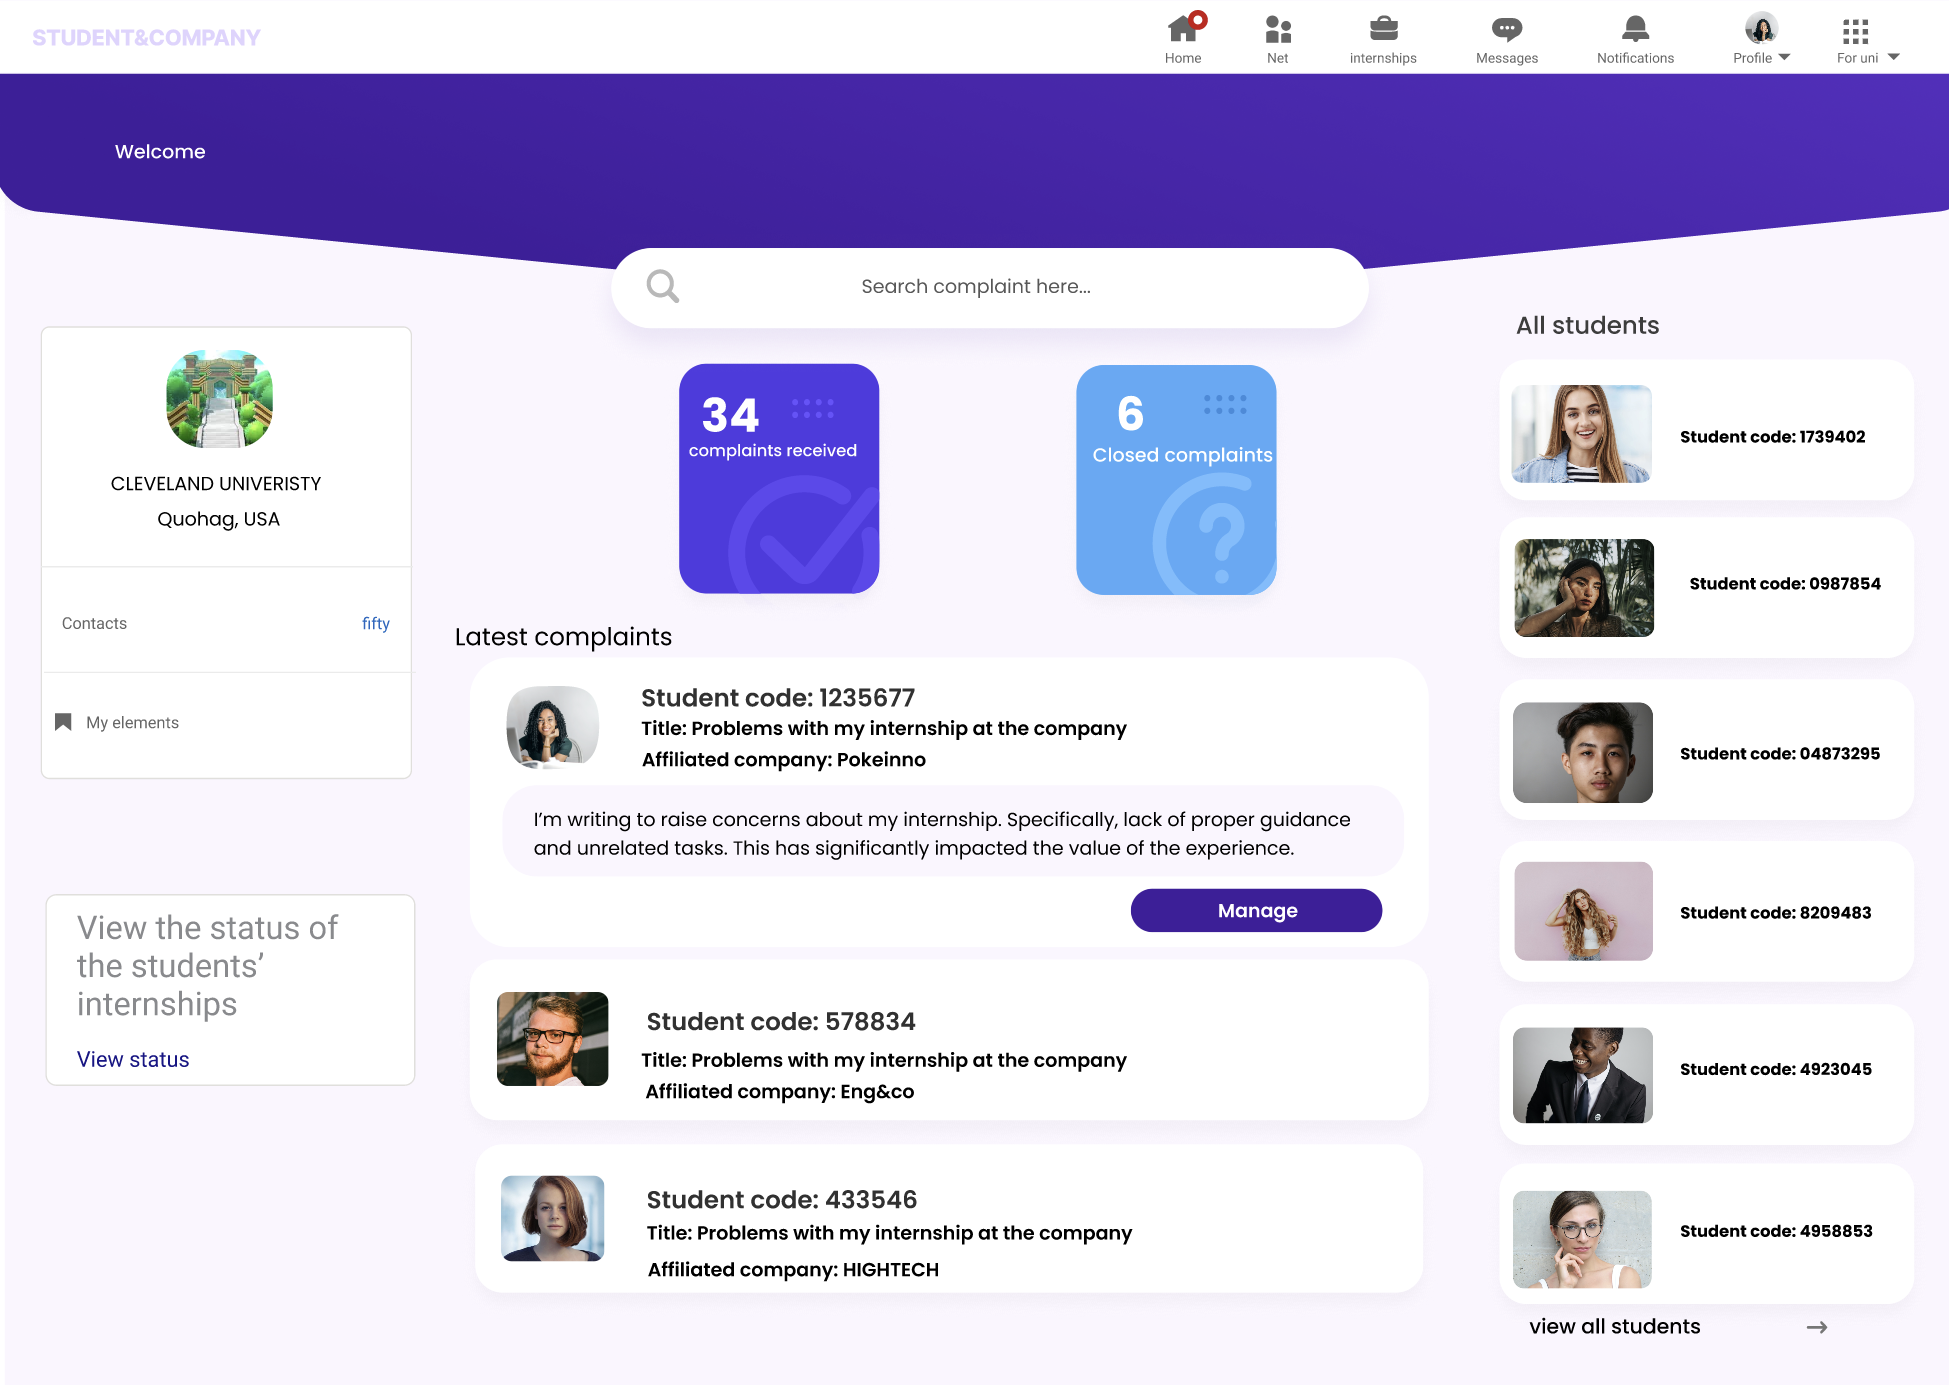
\includegraphics[width=0.5\linewidth]{Interface Images/university interface/Screenshot 2024-12-12 045335.png}
    \caption{University Home page}
    \label{fig: University Home page}
\end{figure}


By clicking on a complaint, the university can respond directly by sending a reply message to the user who submitted it [Figure \ref{fig:Complaints visualization}].

\begin{figure} [H]
    \centering
    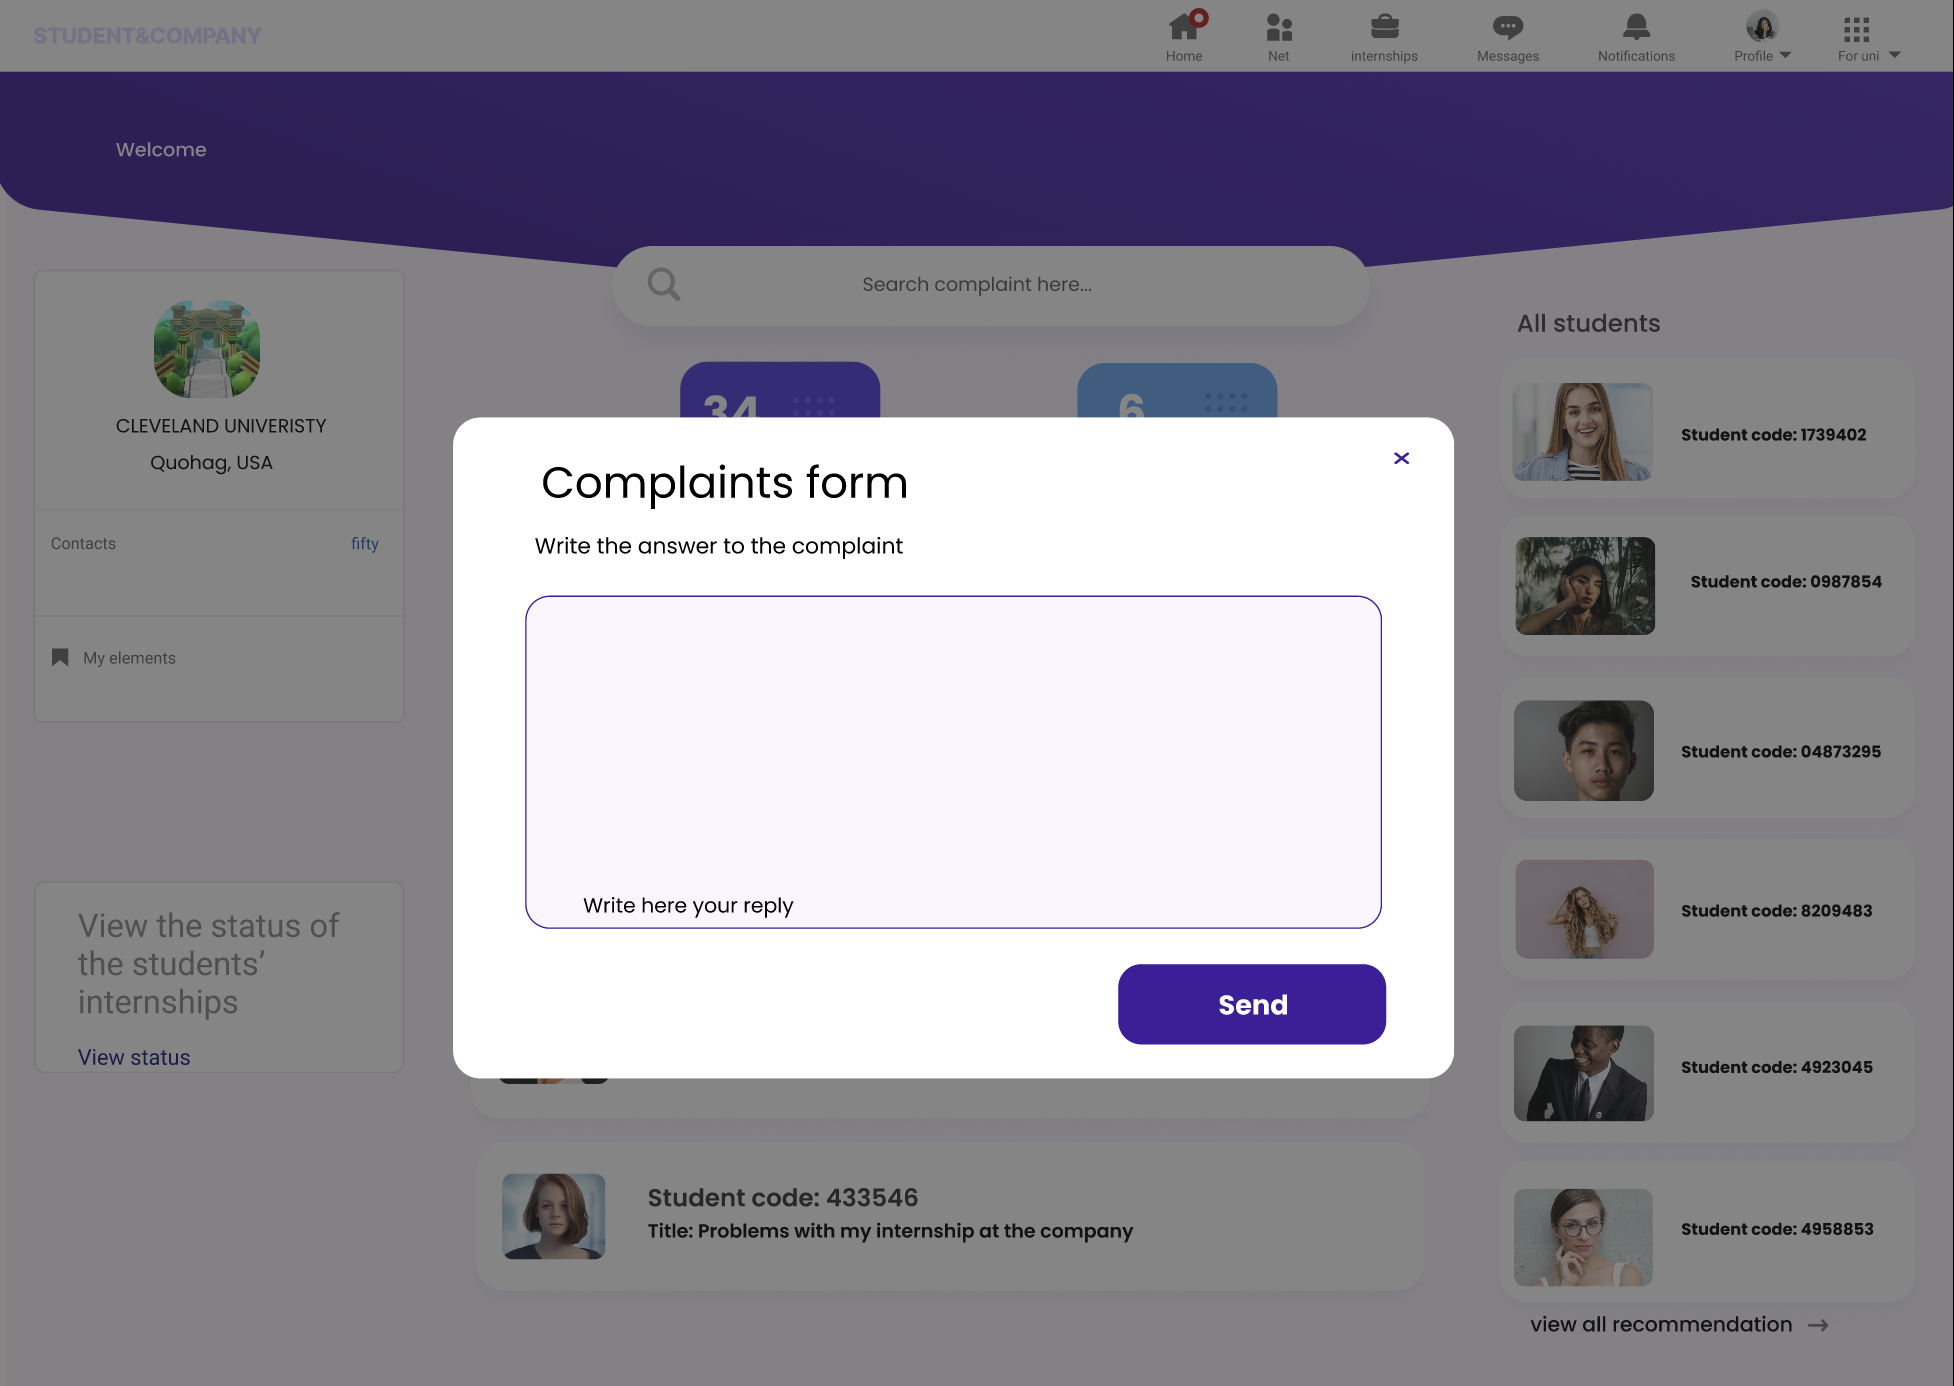
\includegraphics[width=0.5\linewidth]{Interface Images/university interface/Screenshot 2024-12-12 050002.png}
    \caption{Complaints visualization}
    \label{fig:Complaints visualization}
\end{figure}


Complaints are managed through a chat between the university and the involved users, allowing the university to act as an intermediary. This enables the university to assist in resolving the issue or, if necessary, proceed with the conclusion of the internship [Figure \ref{fig: Complaints handling}]

\begin{figure} [H]
    \centering
    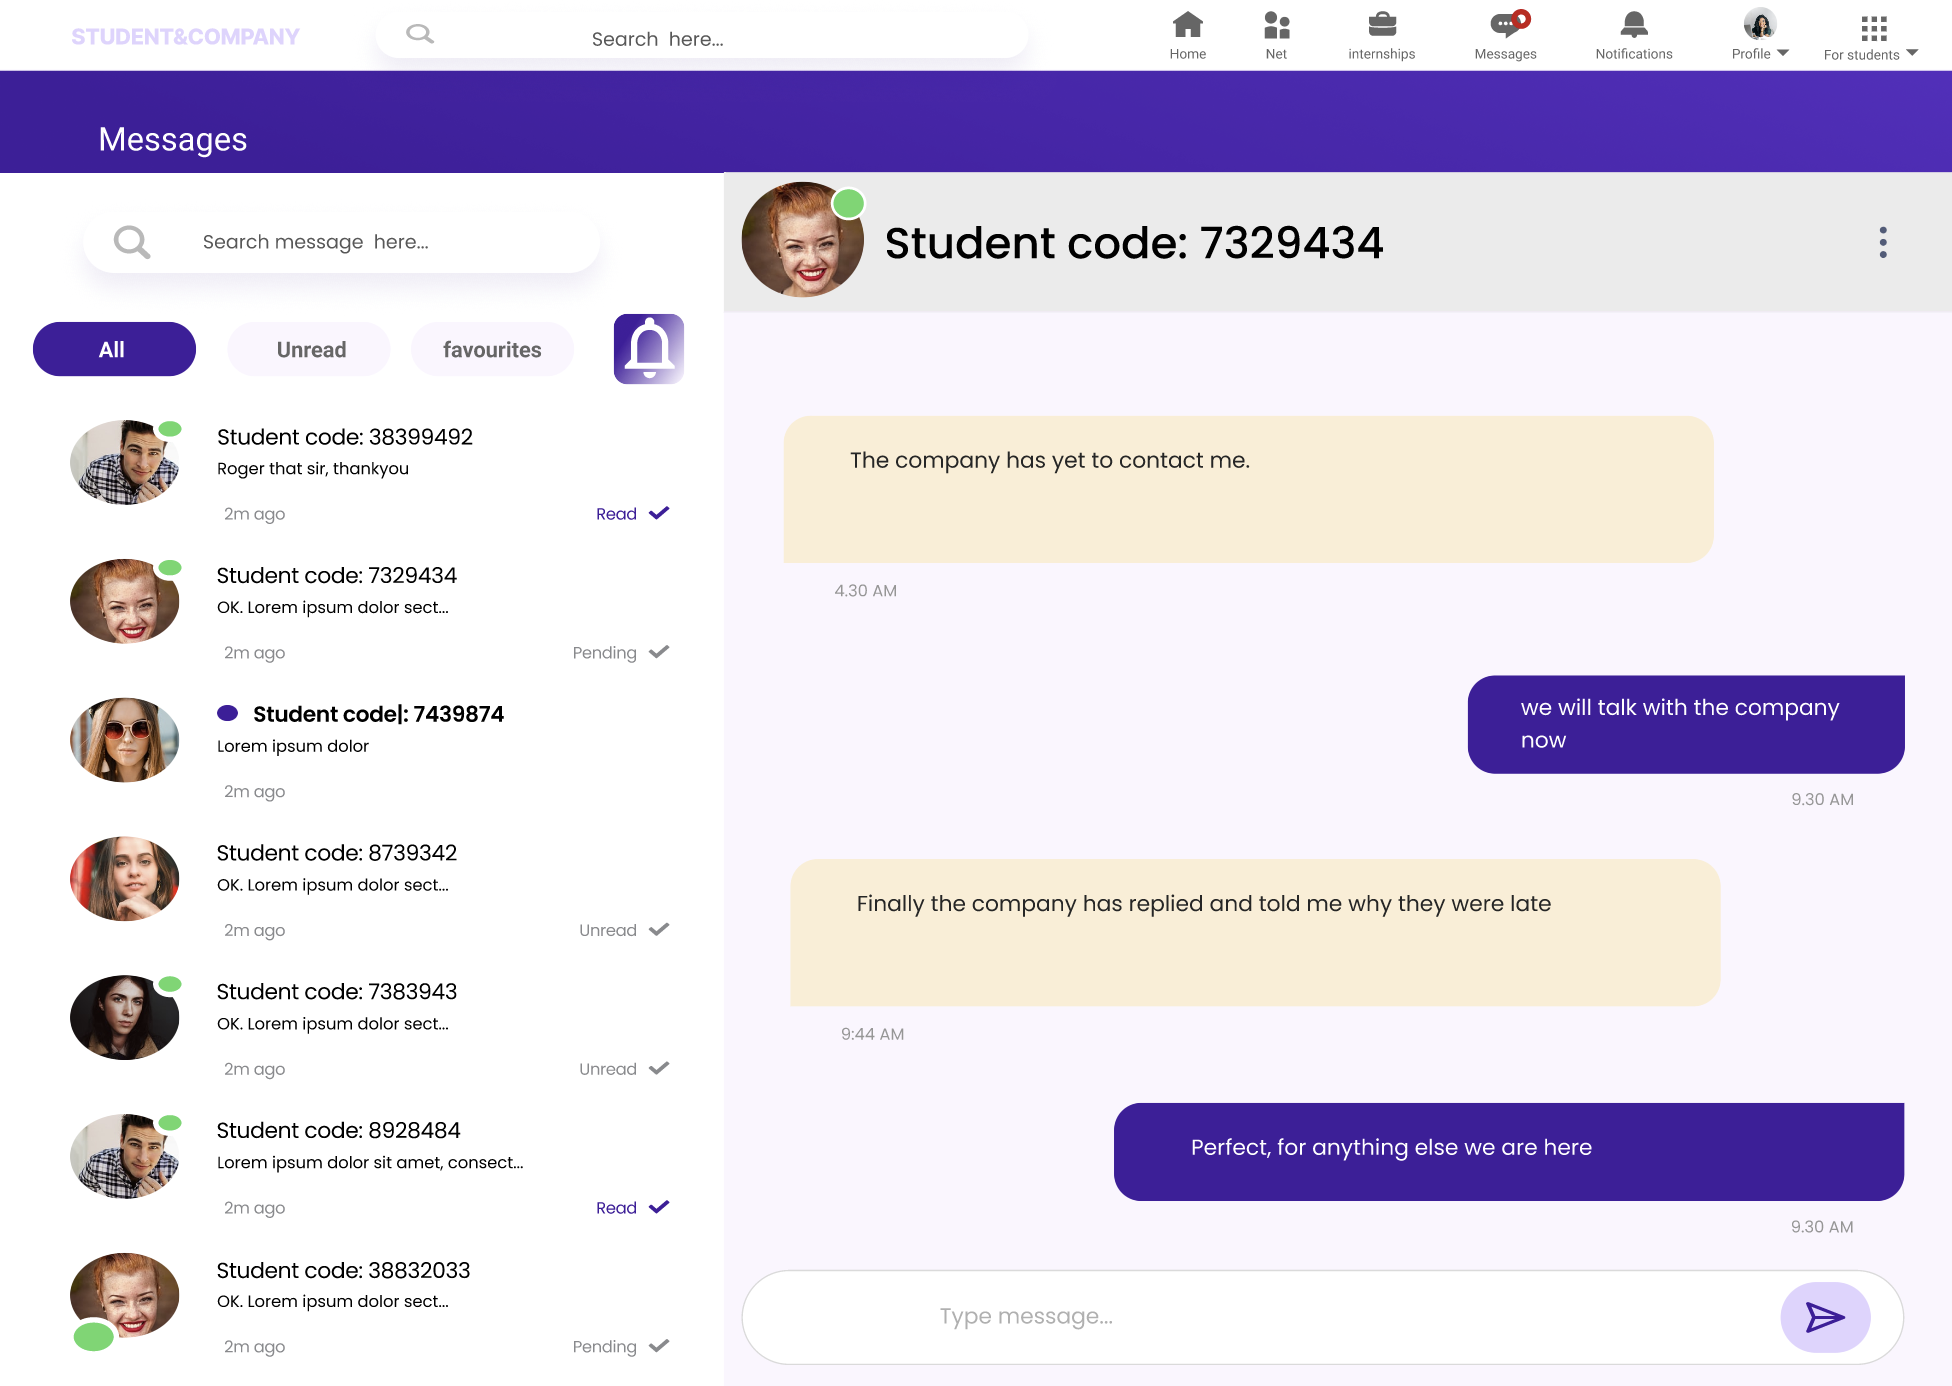
\includegraphics[width=0.5\linewidth]{Interface Images/university interface/Screenshot 2024-12-12 050017.png}
    \caption{Complaints handling}
    \label{fig: Complaints handling}
\end{figure}

\subsection{Common Interfaces}

By clicking on the designated button, users can view all notifications related to important updates, such as changes in internship details, application status, or new internship opportunities that may be of interest to students [Figure \ref{fig:Notifications}].

\begin{figure} [H]
    \centering
    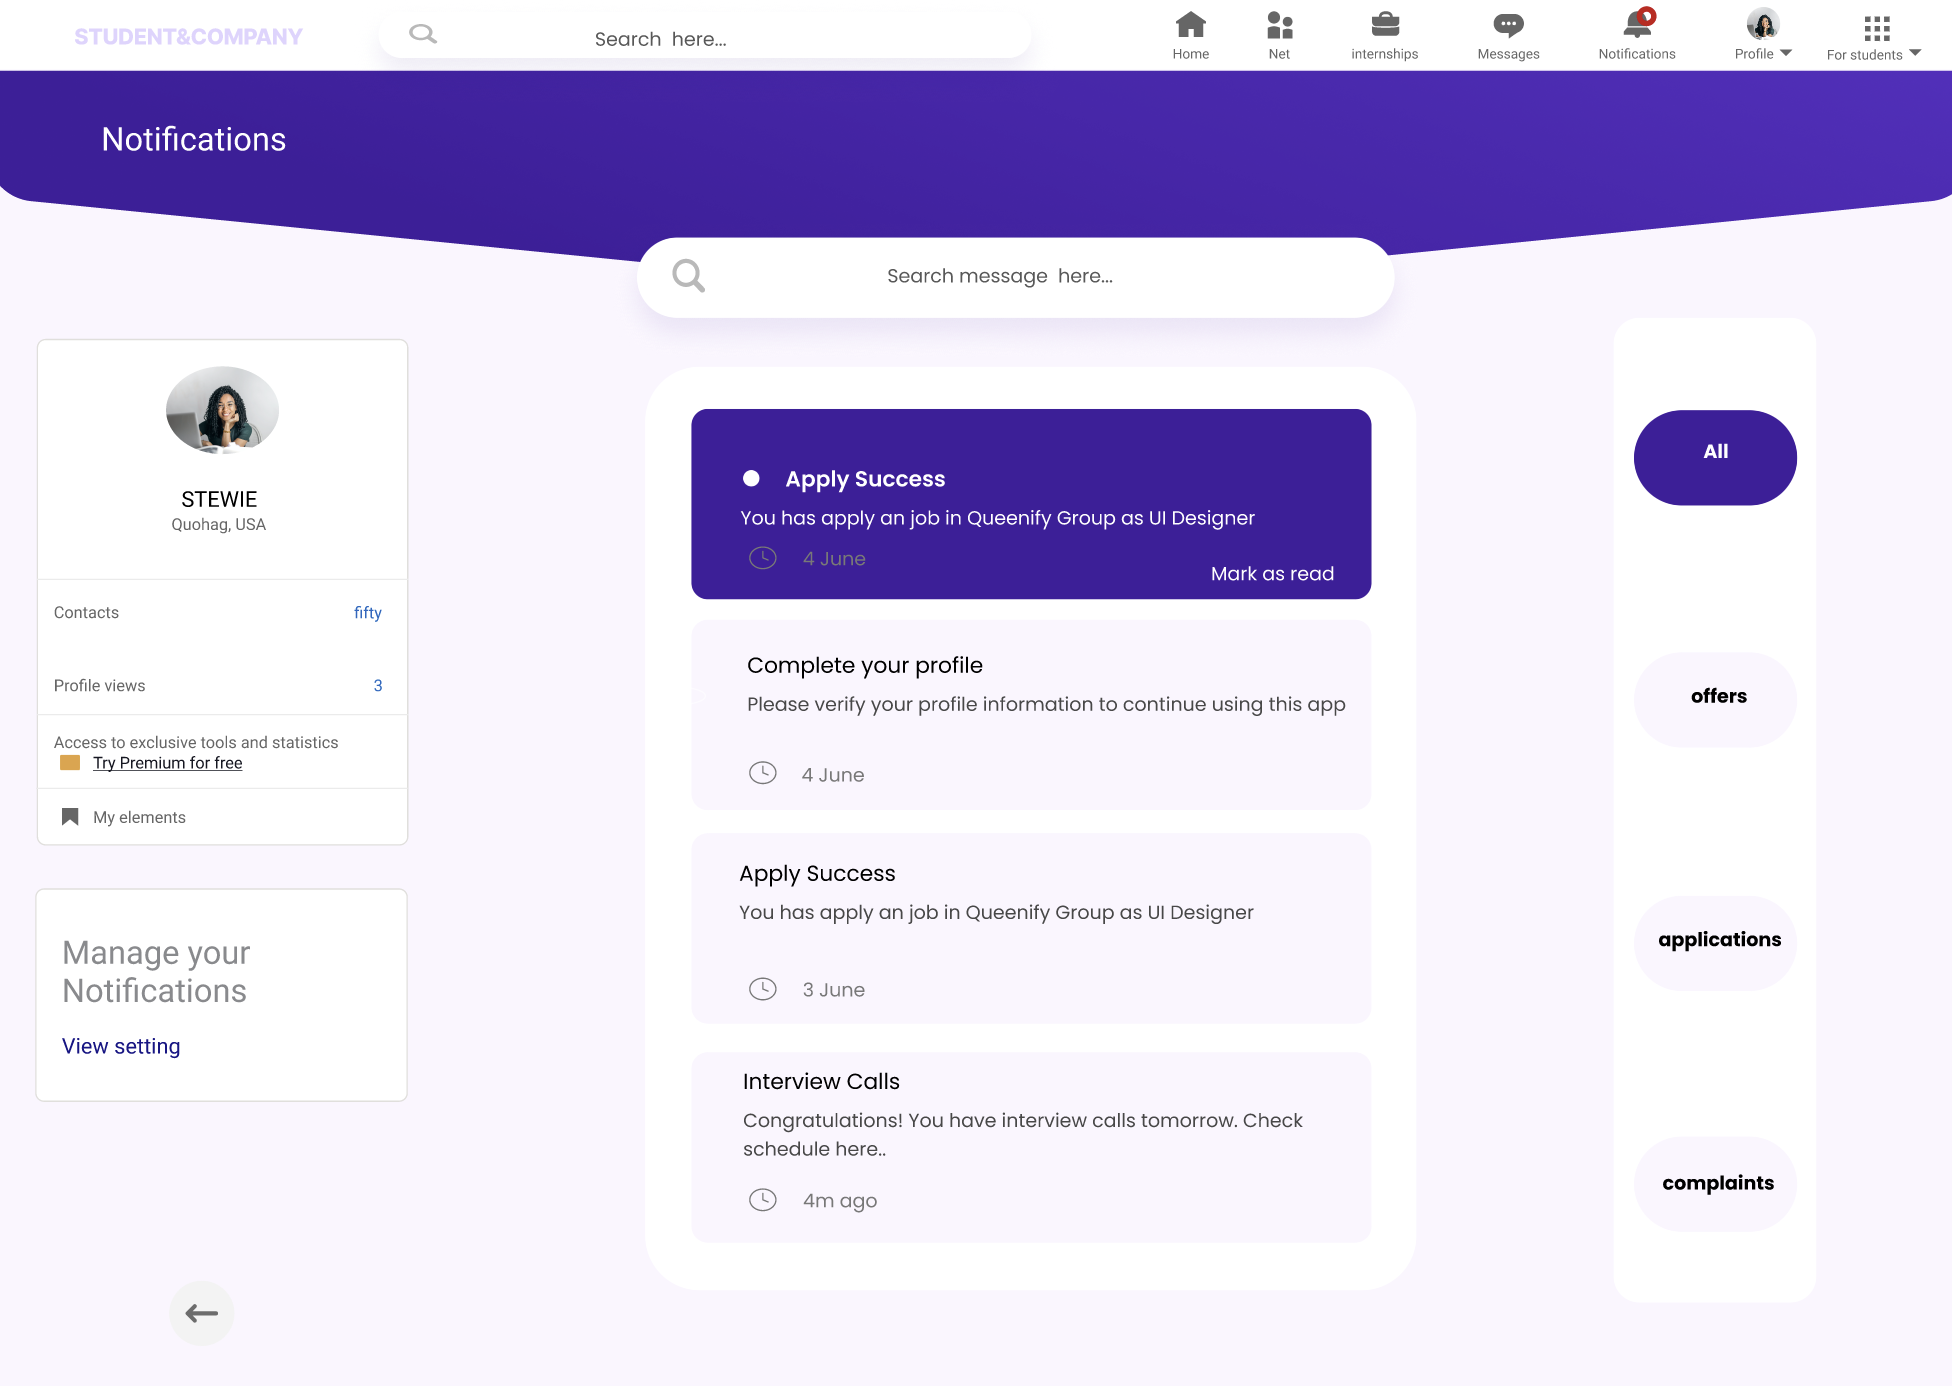
\includegraphics[width=0.5\linewidth]{Interface Images/user interface/Screenshot 2024-12-12 045804.png}
    \caption{Notifications}
    \label{fig:Notifications}
\end{figure}


Users can communicate with each other through a messaging system provided by the platform. Students and companies can interact to discuss internship details, while the university can also use the system to address any complaints or concerns [Figure \ref{fig: Messages}].


\begin{figure} [H]
    \centering
    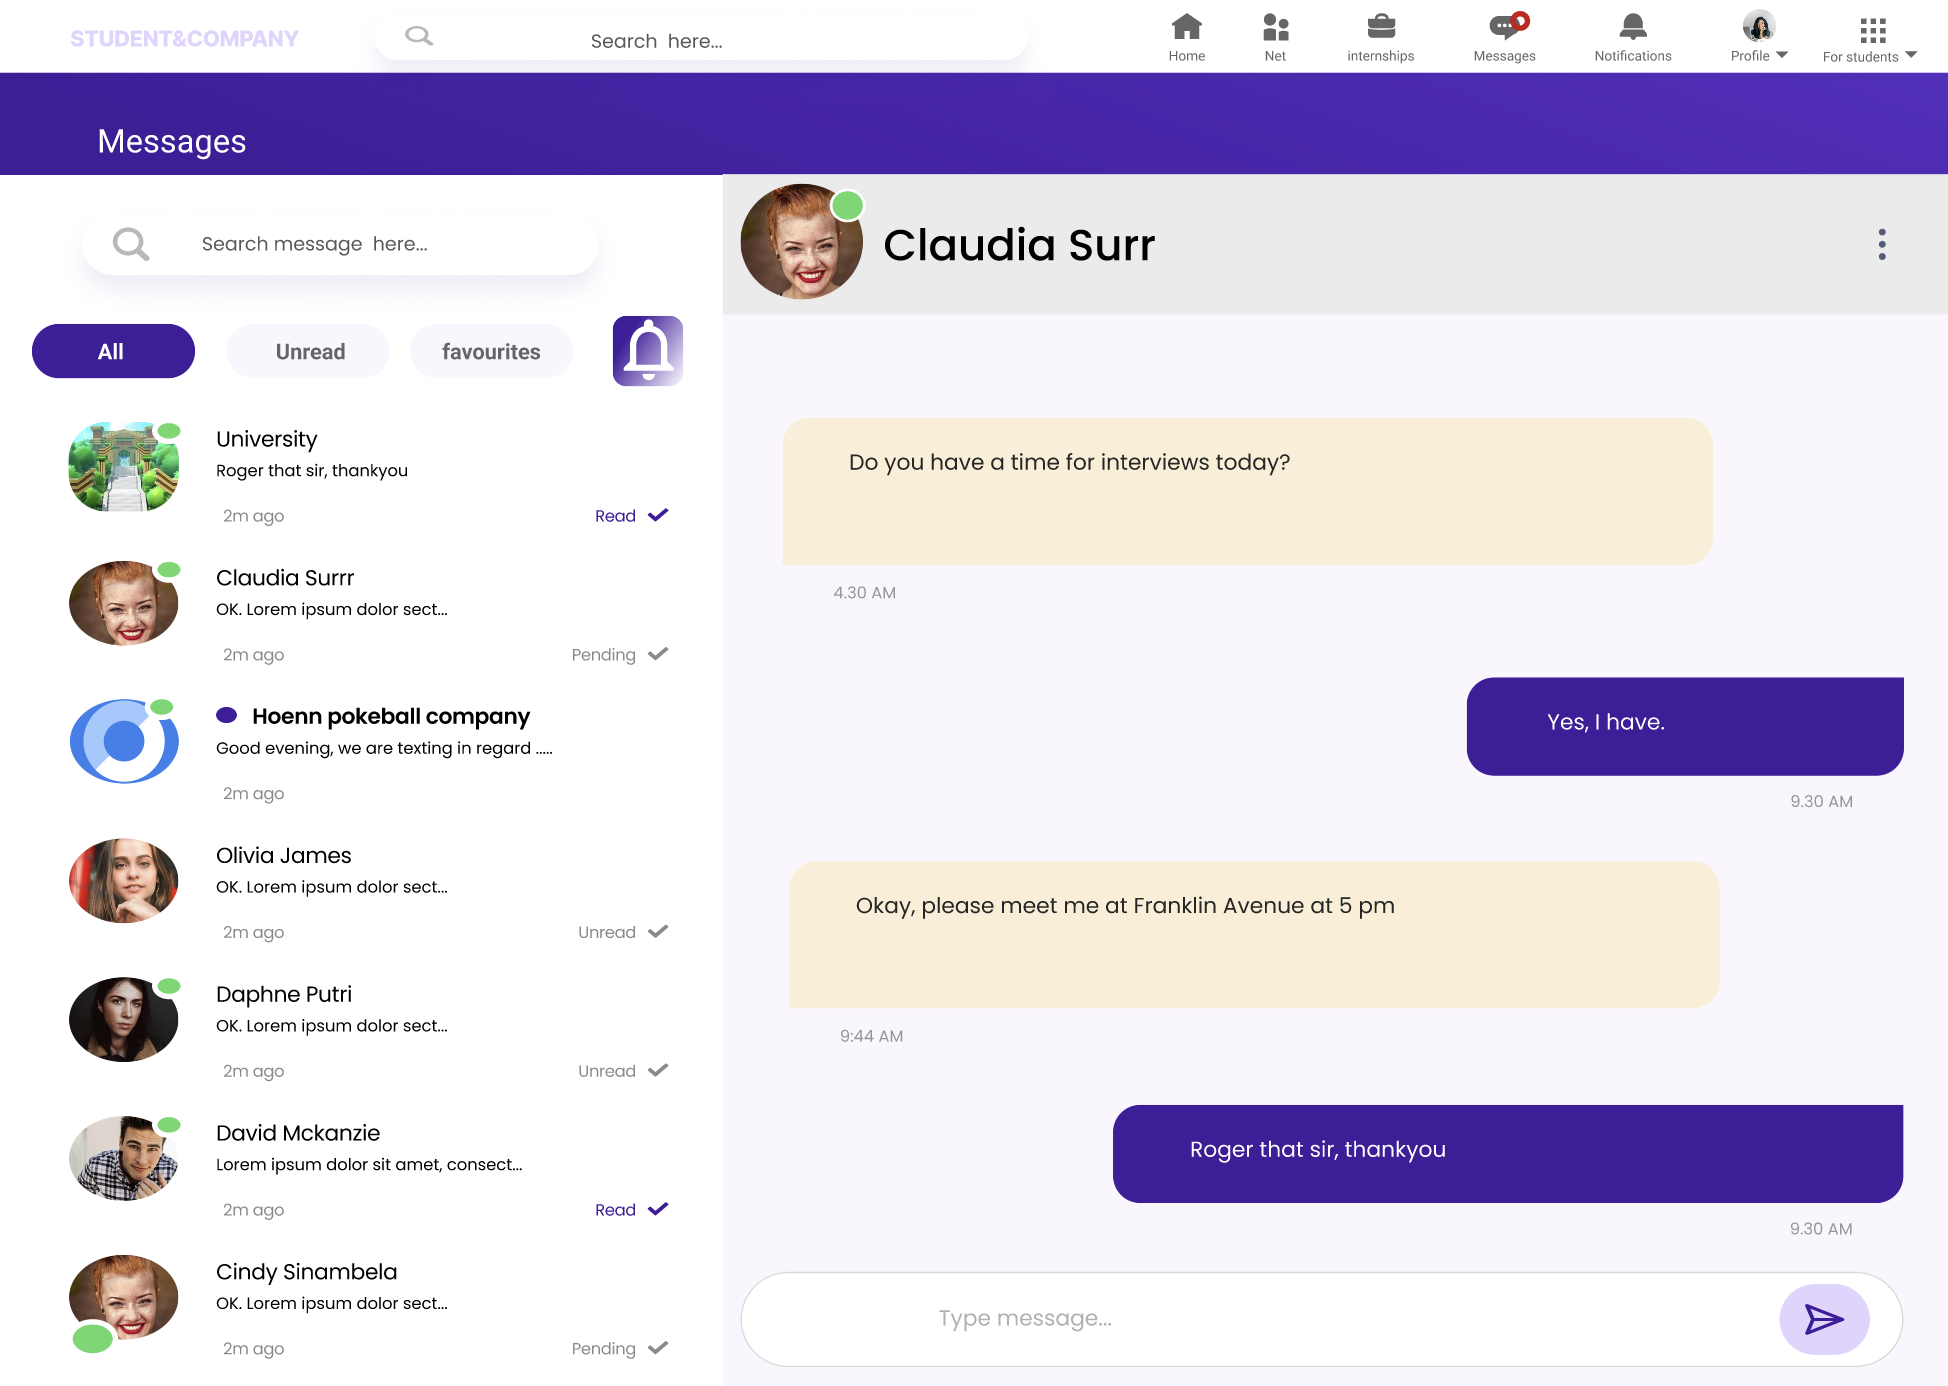
\includegraphics[width=0.5\linewidth]{Interface Images/user interface/Screenshot 2024-12-12 045915.png}
    \caption{Messages}
    \label{fig: Messages}
\end{figure}


Students and companies can also receive feedback requests about their general experience with the platform, provide their own feedback, or submit complaints regarding the progress of the internship once it has started [Figure \ref{fig:Feedback Request}, \ref{fig: Complaints sending}] 

\begin{figure} [H]
    \centering
    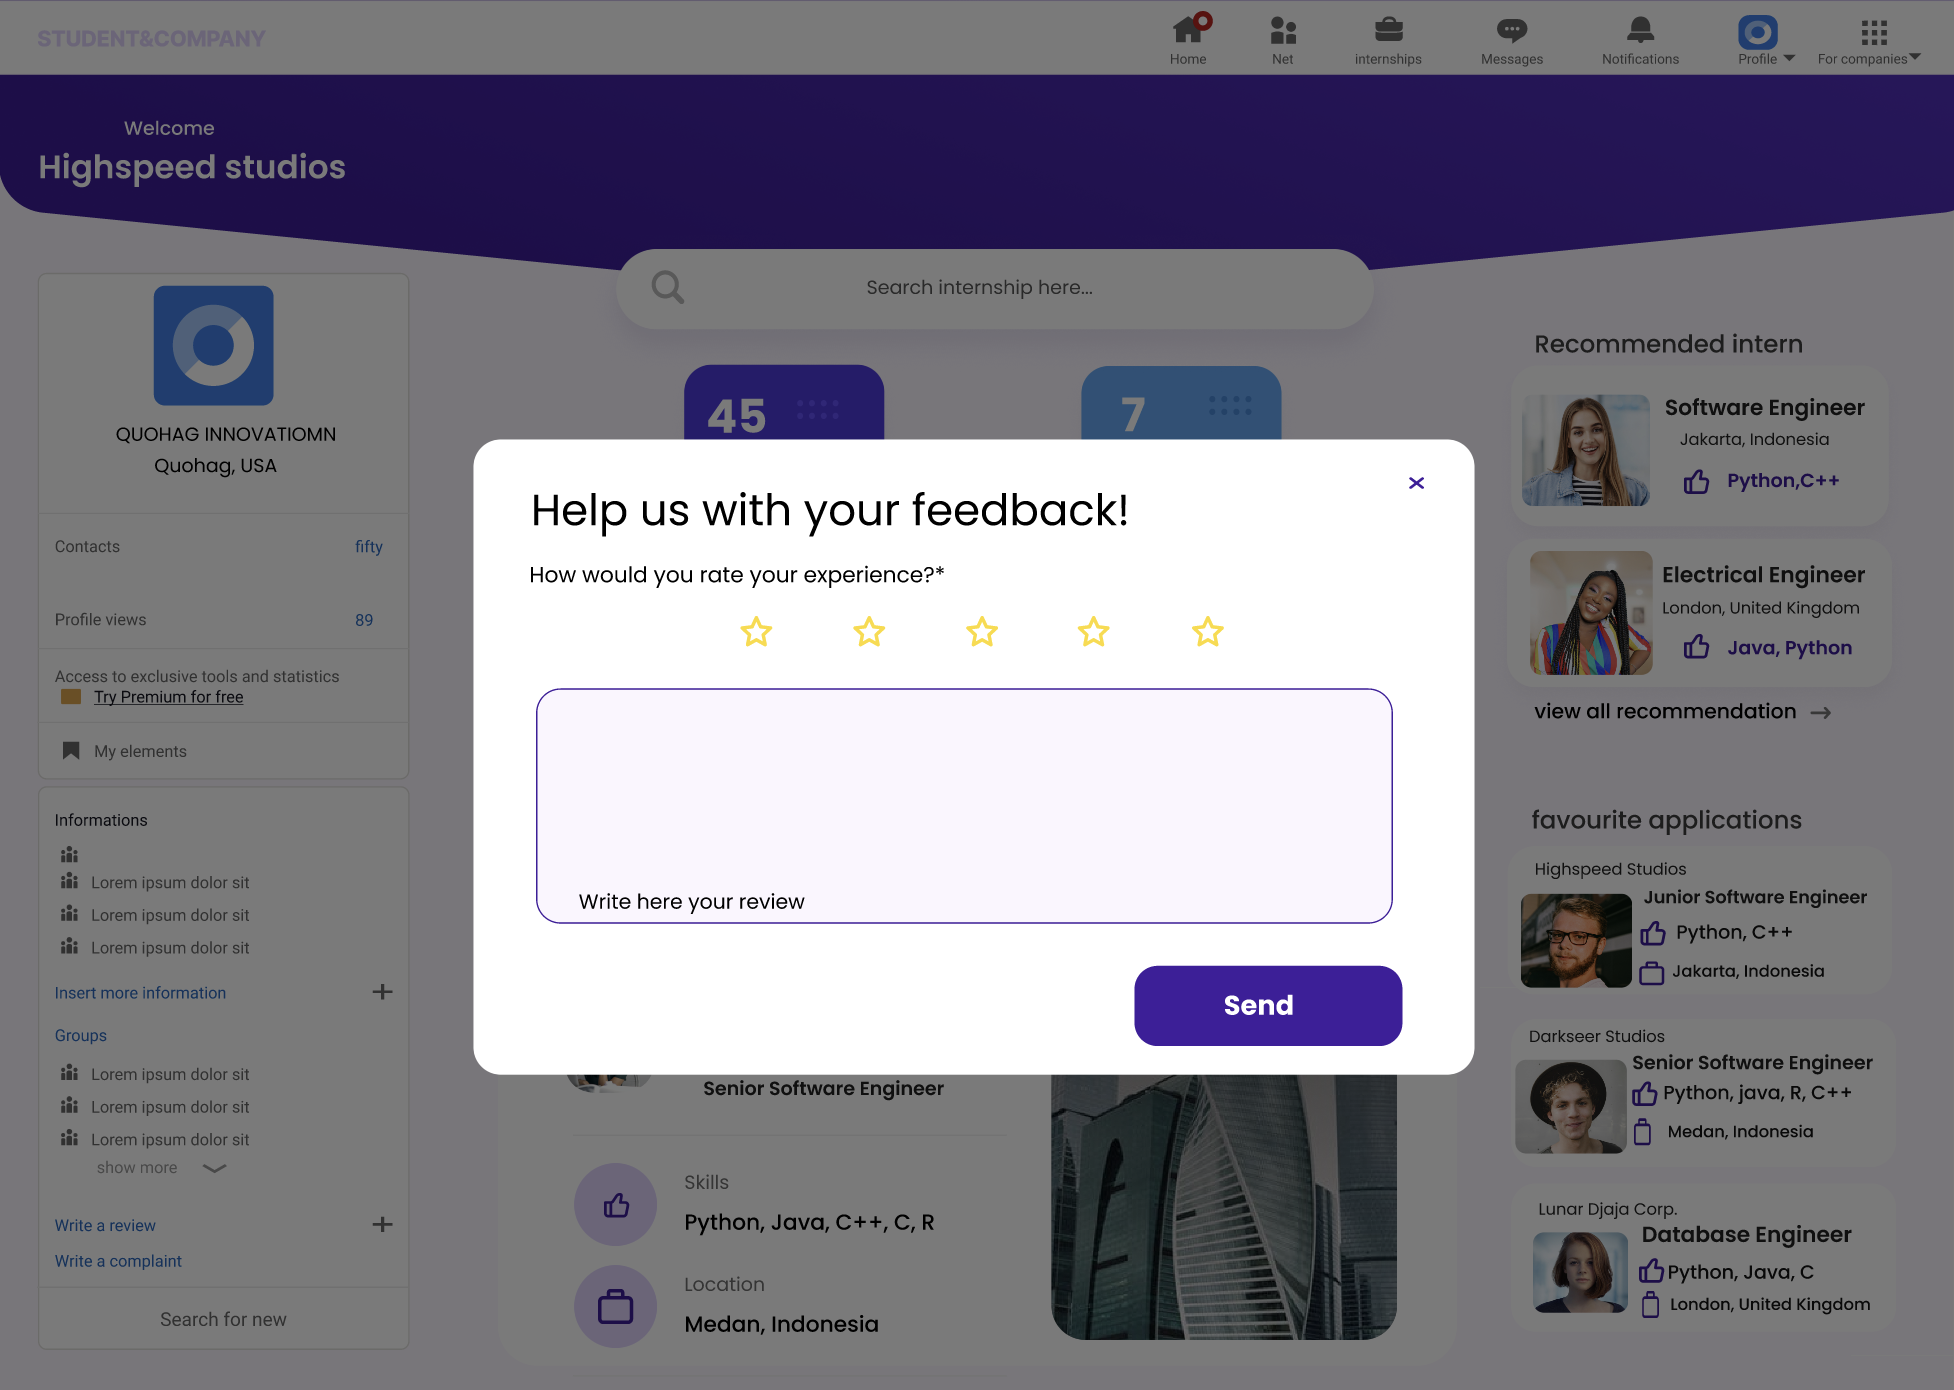
\includegraphics[width=0.5\linewidth]{Interface Images/user interface/Screenshot 2024-12-12 045929.png}
    \caption{Feedback Request}
    \label{fig:Feedback Request}
\end{figure}

\begin{figure} [H]
    \centering
    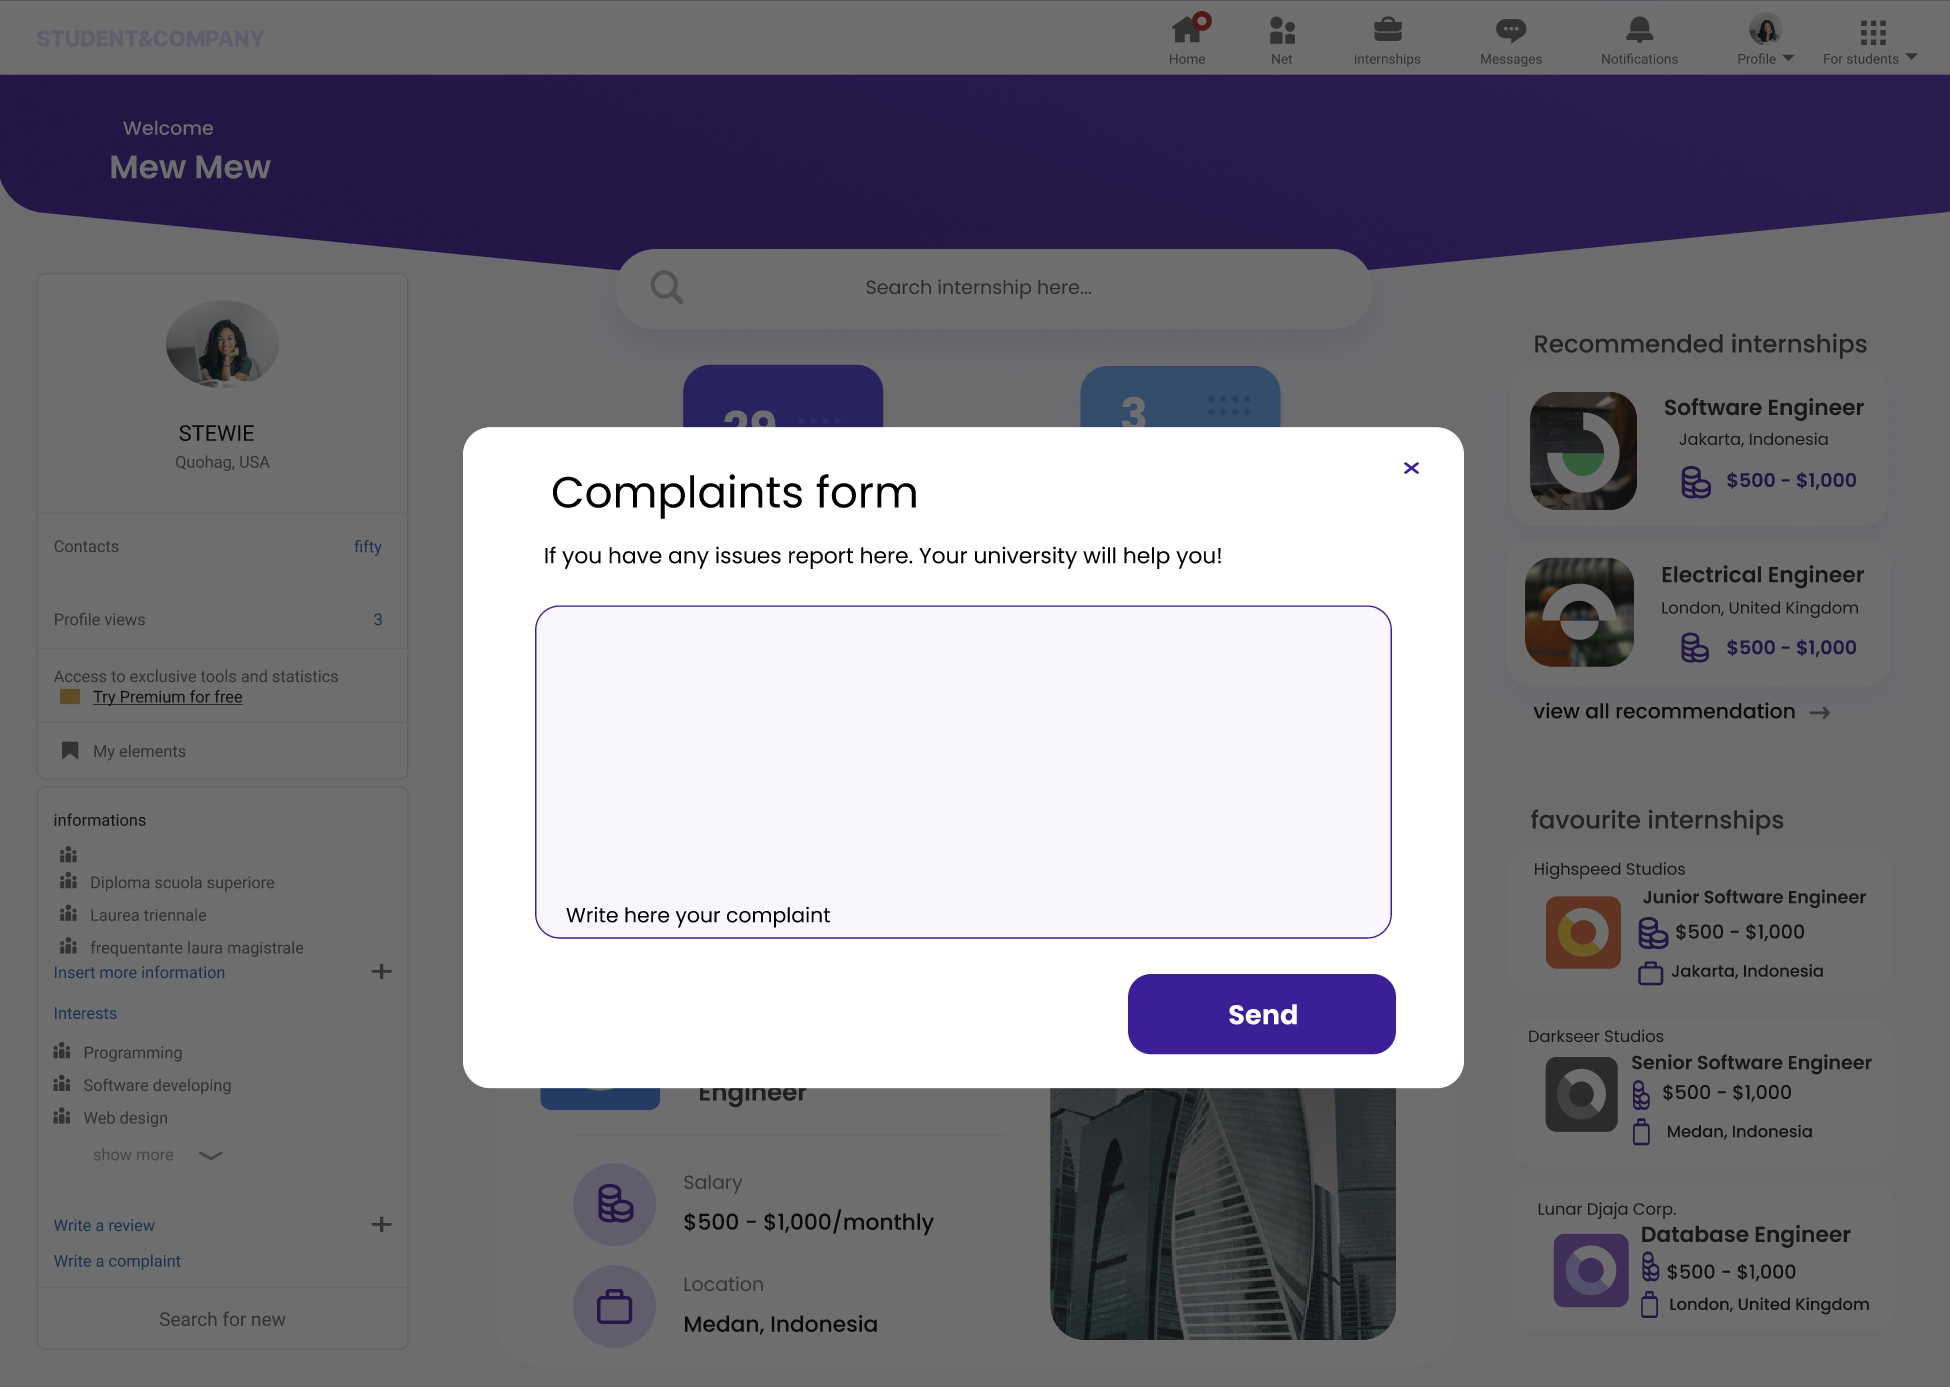
\includegraphics[width=0.5\linewidth]{Interface Images/user interface/Screenshot 2024-12-12 045947.png}
    \caption{Complaints sending}
    \label{fig: Complaints sending}
\end{figure}

\newpage
\section{Functional Requirements}

\subsubsection*{Sign up and log in}
\begin{enumerate}[label={\textbf{[R\arabic*]}}, leftmargin=1.35cm]
    \item The system allows unregistered users to sign up
    \item The system allows users to log in
\end{enumerate}

\subsubsection*{Profile management}
\begin{enumerate}[label={\textbf{[R\arabic*]}}, leftmargin=1.35cm]
    \setcounter{enumi}{2}
    \item The system allows students to insert personal information for the creation of the CV
    \item The system allows companies to insert information for the creation of the internship
    \item The system allows users to update their personal profiles
    \item The system allows companies to view a student's personal profile
    \item The system allows users to retrieve all modified information
    \item The system takes information from the student's personal profile
    \item The system allows a student to see a company’s profile
\end{enumerate}

\subsubsection*{Application management}
\begin{enumerate}[label={\textbf{[R\arabic*]}}, leftmargin=1.35cm]
    \setcounter{enumi}{9}
    \item The system changes the status of the evaluation after updates in the application process
    \item The system allows students to accept the outcome of the evaluation
    \item The system allows companies to evaluate students'applications
\end{enumerate}

\subsubsection*{Internship management}
\begin{enumerate}[label={\textbf{[R\arabic*]}}, leftmargin=1.35cm]
    \setcounter{enumi}{12}
    \item The system displays all the available internships 
    \item The system displays all the information of each specific internship
    \item The system displays specific internships that better suit a student based on the information provided
    \item The system allows students to visualize information about the internship
    \item The system allows a registered student to select an internship to apply to
    \item The system allows users to apply to an internship
    \item The system allows companies to set up evaluation criteria
    \item The system allows universities to set up criteria for internship's conclusion
\end{enumerate}

\subsubsection*{Complaints management}
\begin{enumerate}[label={\textbf{[R\arabic*]}}, leftmargin=1.35cm]
    \setcounter{enumi}{20}
    \item The system allows users to name other parties involved in the complaint
    \item The system displays the complaints sent by both students and companies
    \item The system updates the status of a complaint
    \item The system allows universities to close an internship
\end{enumerate}

\subsubsection*{Messages and Notifications}
\begin{enumerate}[label={\textbf{[R\arabic*]}}, leftmargin=1.35cm]
    \setcounter{enumi}{24}
    \item The system asks users for permission to send messages
    \item The system generates a message of confirmation after an operation is done
    \item The system generates a message once the status of the internship changes
    \item The system allows users to retrieve all messages sent
    \item The system generates suggestions based on the information taken in the platform
\end{enumerate}

\subsubsection*{Feedback}
\begin{enumerate}[label={\textbf{[R\arabic*]}}, leftmargin=1.35cm]
    \setcounter{enumi}{29}
    \item The system allows students and companies to provide feedback
    \item The system generated a feedback request to send to students and companies
\end{enumerate}


\subsection{Use Cases Diagram}
\begin{figure} [H]
    \centering
    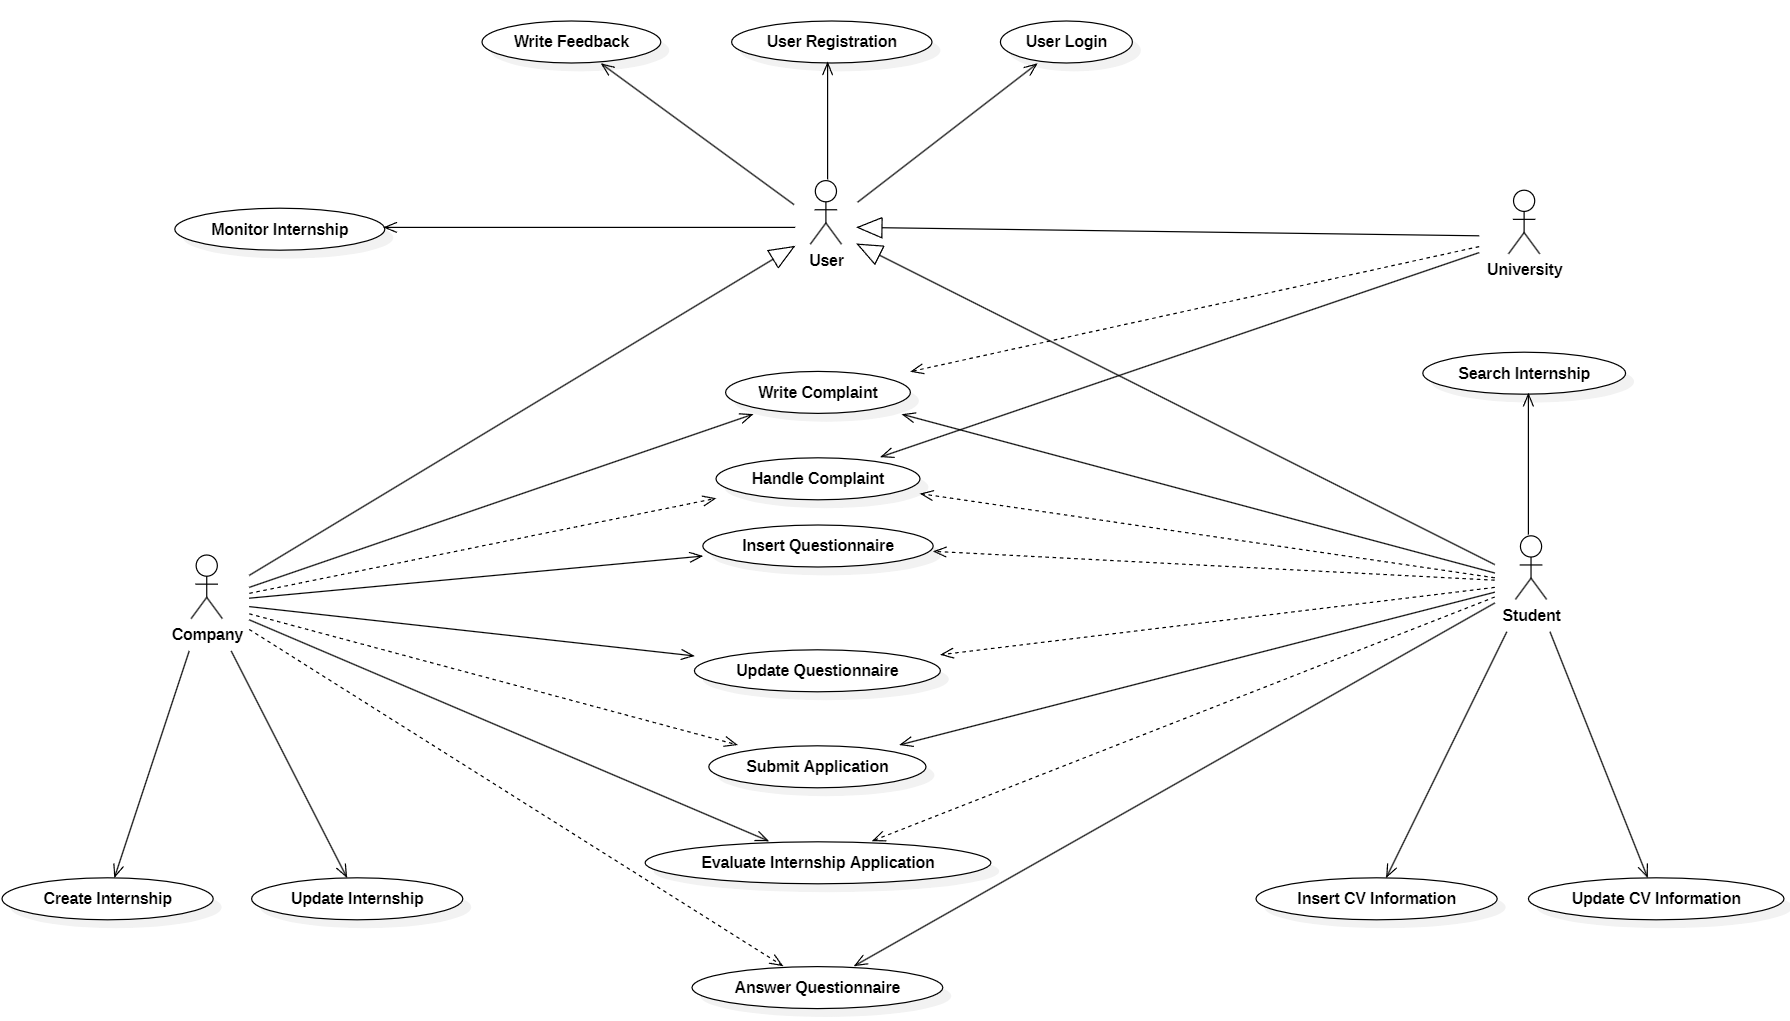
\includegraphics[width=1\linewidth]{Use Cases Images/use_case_diagram.png}
    \label{fig: User Cases Diagram}
\end{figure}

\newpage
\subsection{Use Case}

\subsubsection*{User Registration}
\begin{table}[H]
    \centering
    \renewcommand{\arraystretch}{1.5}
    \begin{tabular}{|p{4cm}|p{11cm}|}
    \hline
    \rowcolor{bluepoli!40}
    \textbf{[UC1]} & \textbf{User Registration} \\ \hline \hline
    \textbf{Actors} & User \\ \hline
    \textbf{Entry Condition} & / \\ \hline
    \textbf{Input} & All the necessary information required by the system, like name, password, mail, etc. \\ \hline
    \textbf{Event Flow} & 
    {\setlength{\leftmargini}{1.4em}
    \begin{enumerate}
        \item The user enters on the platform.
        \item The user clicks on the "Sign In" button.
        \item The user has to choose to create an account as University, Company, or Student.
        \item The user fills every section with the required information.
        \item The user clicks on the "Register" button.
        \item The system notifies the user.
    \end{enumerate}} \\ \hline
    \textbf{Exit Condition} & The account is created by the system. \\ \hline
    \textbf{Output} & The user receives a message confirming the creation of the account. \\ \hline
    \textbf{Exceptions} & 
    {\setlength{\leftmargini}{1.1em}
    \begin{itemize}
        \item \textbf{Missing Information}: If required fields are not completed, the system prompts the student to fill out all mandatory sections.
        \item \textbf{Existing Mail}: If the mail inserted by the user is already taken, the system prompts an error.
    \end{itemize}} \\ \hline
    \end{tabular}
    \caption{User Registration Table}
\end{table}

\begin{figure} [H]
    \centering
    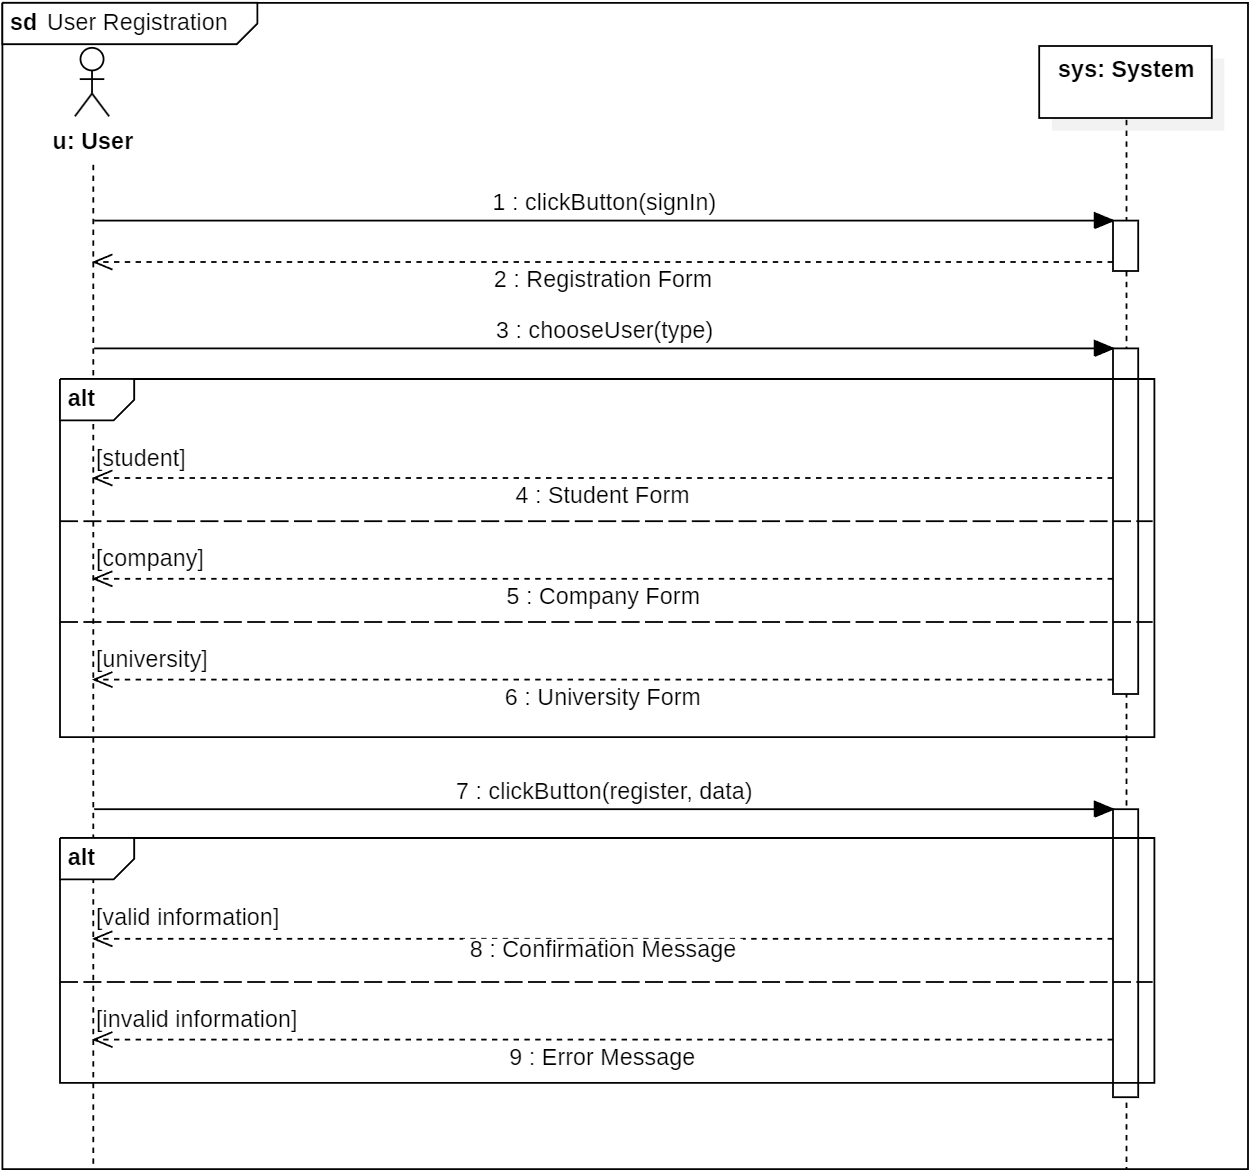
\includegraphics[width=1\linewidth]{Use Cases Images/user_registration.png}
    \caption{Diagram for [UC1]}
    \label{fig: User Registration Diagram}
\end{figure}


\subsubsection*{User Login}
\begin{table}[H]
    \centering
    \renewcommand{\arraystretch}{1.5}
    \begin{tabular}{|p{4cm}|p{11cm}|}
    \hline
    \rowcolor{bluepoli!40}
    \textbf{[UC2]} & \textbf{User Login} \\ \hline \hline
    \textbf{Actors} & User \\ \hline
    \textbf{Entry Condition} & The user is registered \\ \hline
    \textbf{Input} & Mail and passwords associated with the account \\ \hline
    \textbf{Event Flow} & 
    {\setlength{\leftmargini}{1.4em}
    \begin{enumerate}
        \item The user enters on the platform.
        \item The user clicks on the "Login" button.
        \item The user inserts mail and password.
        \item The user clicks on the "Enter" button.
    \end{enumerate}} \\ \hline
    \textbf{Exit Condition} & User is logged in \\ \hline
    \textbf{Output} & / \\ \hline
    \textbf{Exceptions} & 
    \textbf{Wrong information}: If the user enters an email or password that is not in the database, the system prompts the user to verify the information entered. \\ \hline
    \end{tabular}
    \caption{User Login Table}
\end{table}

\begin{figure} [H]
    \centering
    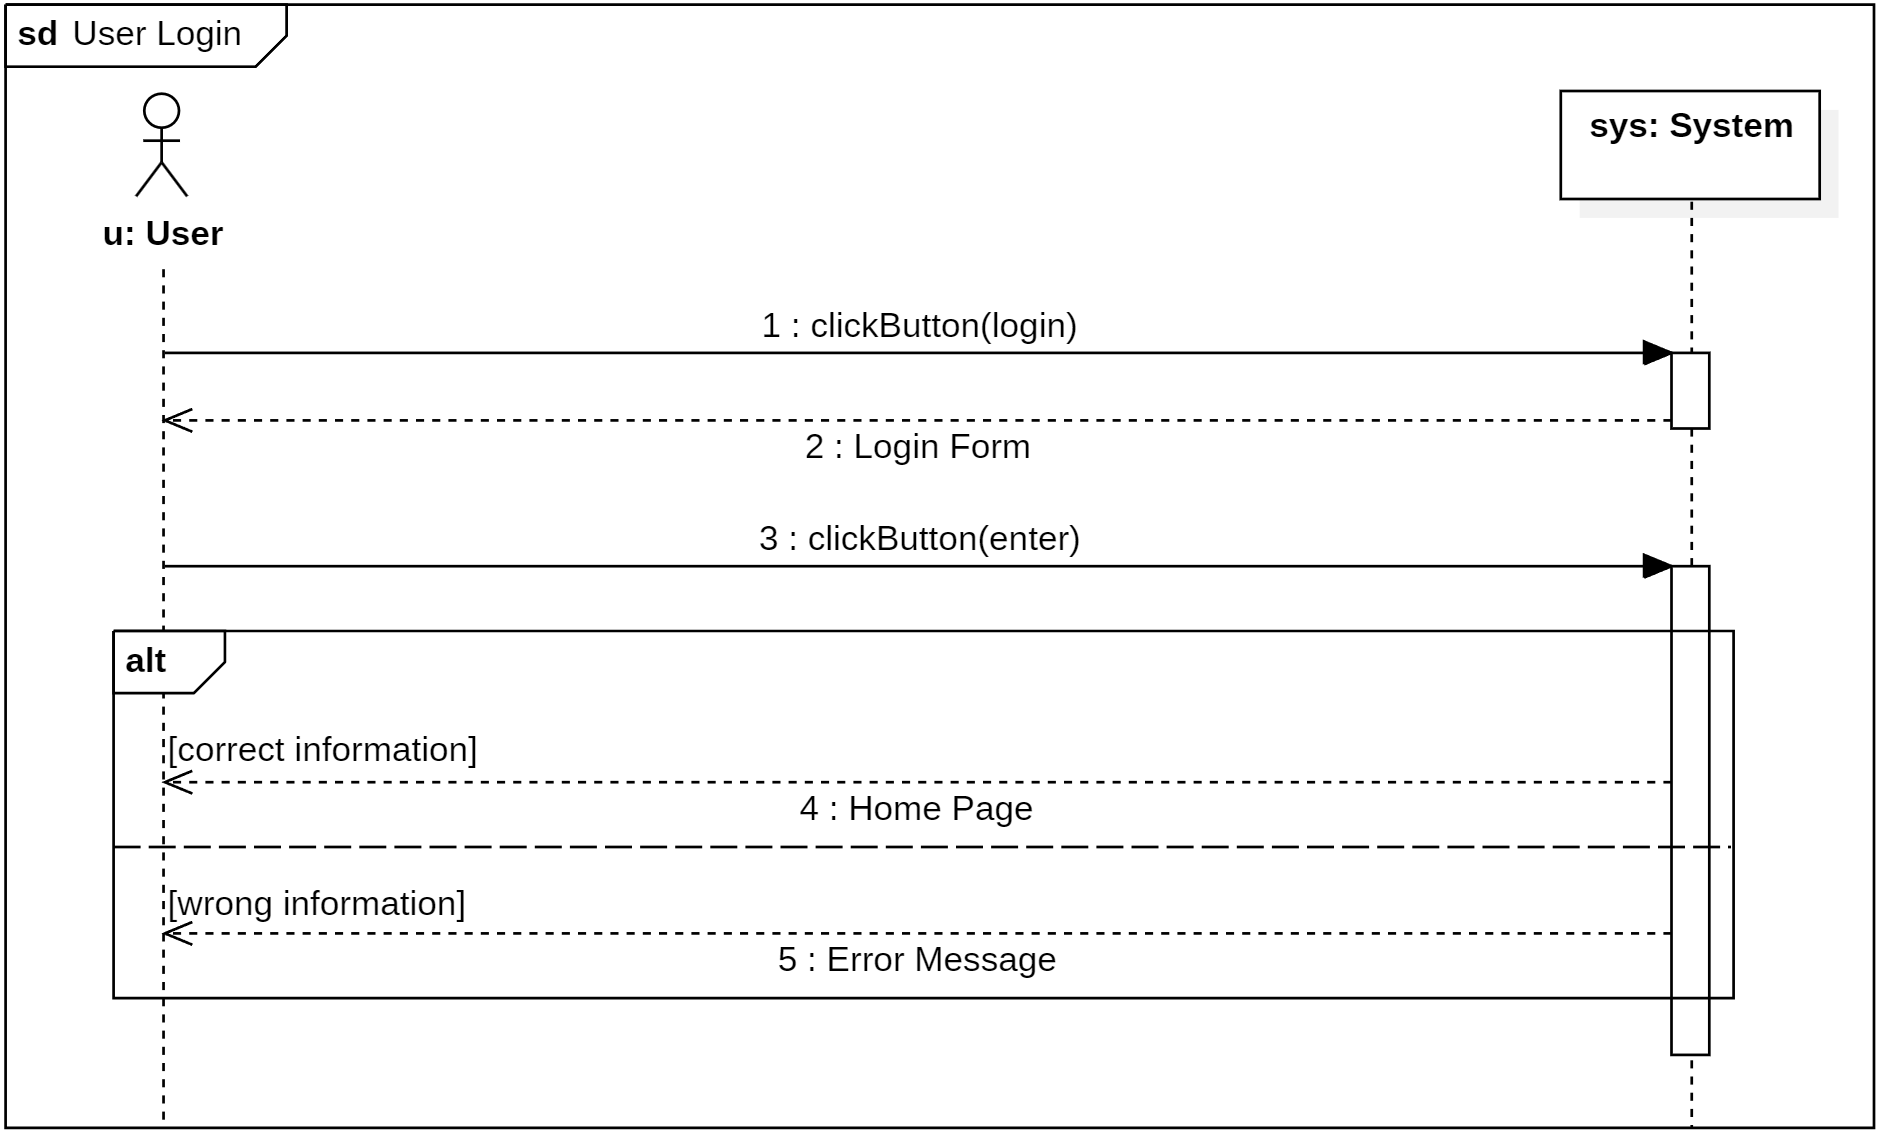
\includegraphics[width=1\linewidth]{Use Cases Images/user_login.png}
    \caption{Diagram for [UC2]}
    \label{fig: User Login Diagram}
\end{figure}

\subsubsection*{Insert CV information}
\begin{table}[H]
    \centering
    \renewcommand{\arraystretch}{1.5}
    \begin{tabular}{|p{4cm}|p{11cm}|}
    \hline
    \rowcolor{bluepoli!40}
    \textbf{[UC3]} & \textbf{Insert CV Information} \\ \hline \hline
    \textbf{Actors} & Student \\ \hline
    \textbf{Entry Condition} & 
    {\setlength{\leftmargini}{1.1em}
    \begin{itemize}
        \item The student is registered.
        \item The student is logged in.
    \end{itemize}} \\ \hline
    \textbf{Input} & 
    All the necessary information for a CV, such as past experiences, skills, education, certifications, etc. \\ \hline
    \textbf{Event Flow} & 
    {\setlength{\leftmargini}{1.4em}
    \begin{enumerate}
        \item The student accesses his profile page.
        \item The student clicks on the "Insert CV" button.
        \item The student fills in the sections with the required information (experiences, skills, etc.).
        \item If he wants, the student clicks on the "Improve" button.
        \item The system provides suggestions to improve the CV.
        \item The student makes adjustments based on the suggestions.
        \item The student clicks on the "Confirm" button.
    \end{enumerate}} \\ \hline
    \textbf{Exit Condition} & 
    {\setlength{\leftmargini}{1.1em}
    \begin{itemize}
        \item The CV information is successfully saved in the system.
        \item The updated CV is now visible in the student's profile.
    \end{itemize}} \\ \hline
    \textbf{Output} & 
    A confirmation message is displayed to the student stating that the CV information has been successfully saved. \\ \hline
    \textbf{Exceptions} & 
    \textbf{Missing Information}: If required fields are not completed, the system prompts the student to fill out all mandatory sections. \\ \hline
    \end{tabular}
    \label{table:example}
    \caption{Insert CV Information Table}
\end{table}

\begin{figure} [H]
    \centering
    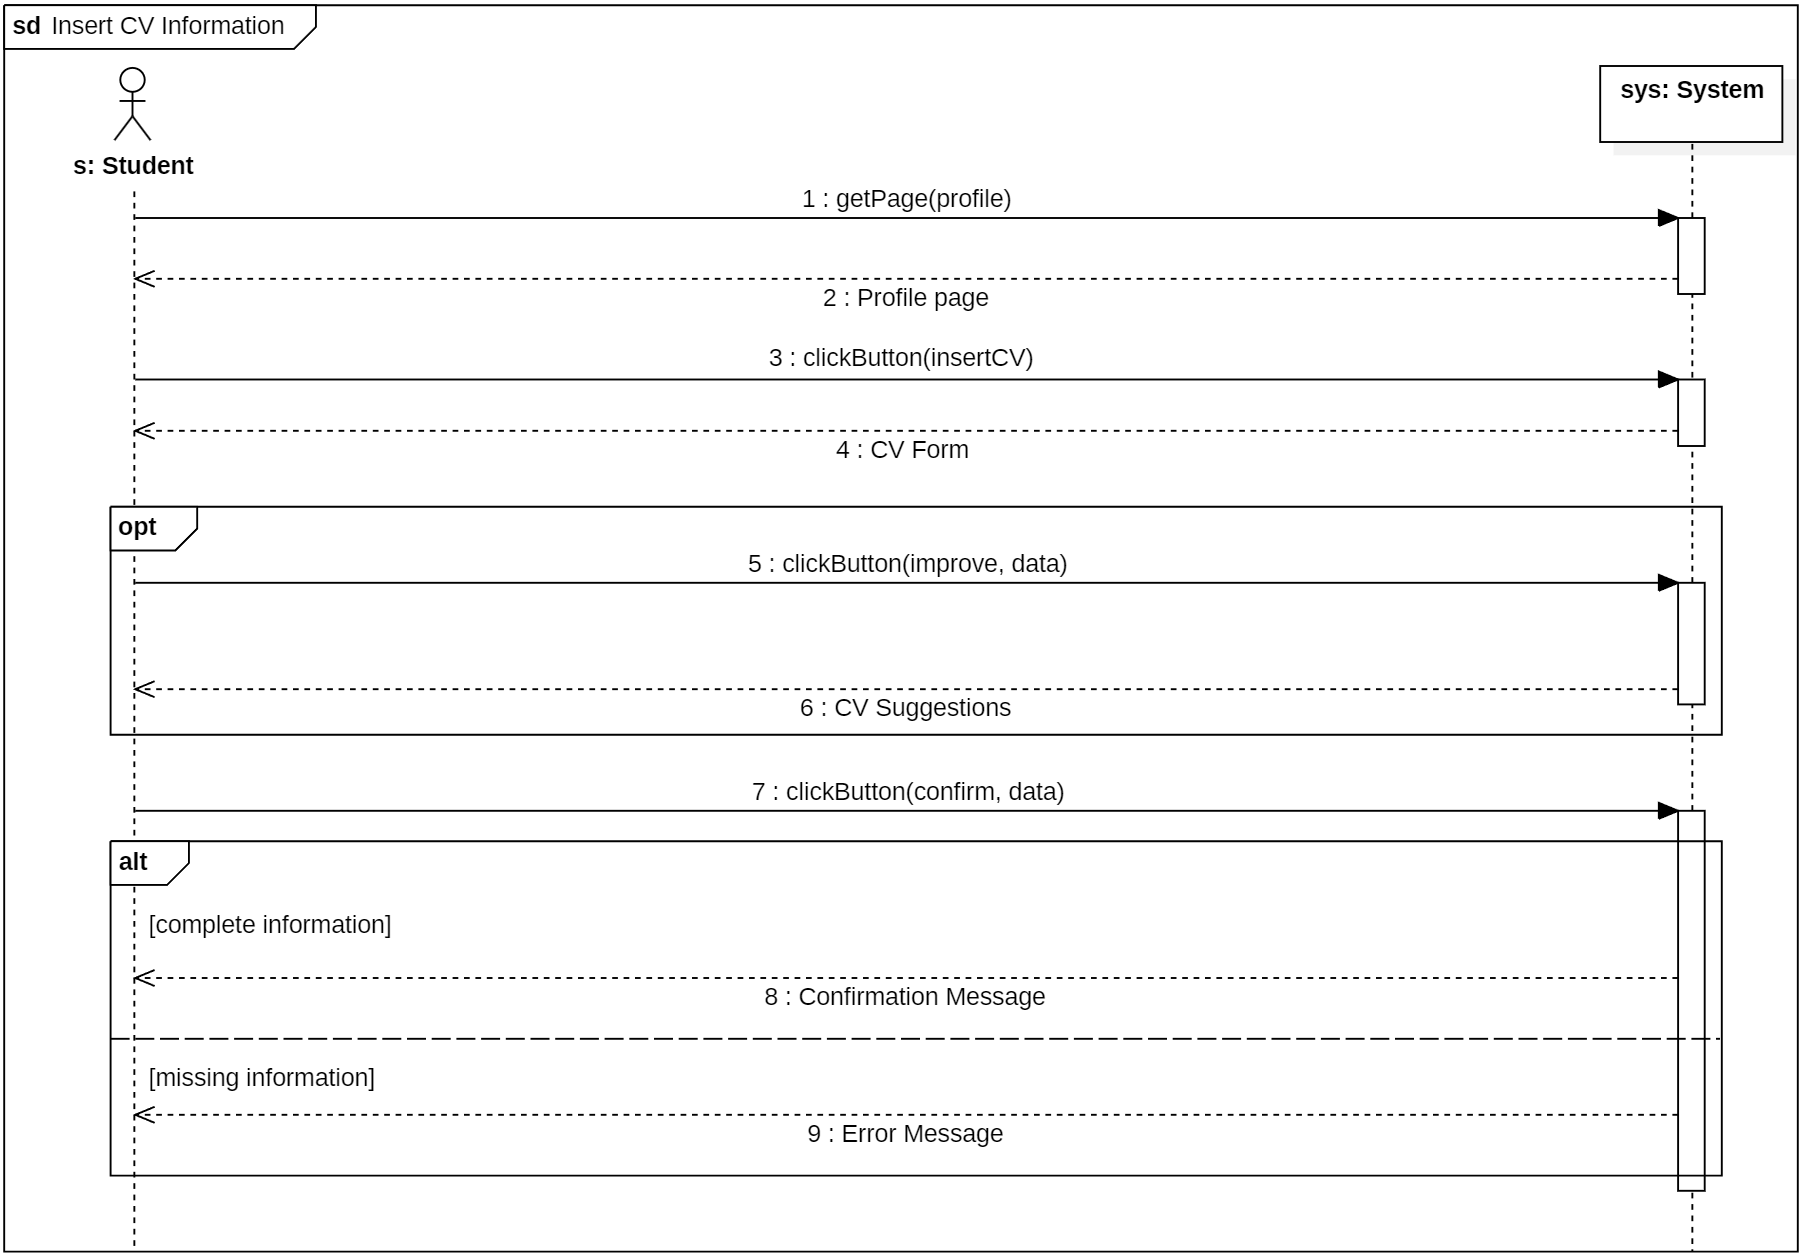
\includegraphics[width=1\linewidth]{Use Cases Images/insert_CV_informations.png}
    \caption{Diagram for [UC3]}
    \label{fig: Insert CV Information Diagram}
\end{figure}

\subsubsection*{Update CV information}
\begin{table}[H]
    \centering
    \renewcommand{\arraystretch}{1.5}
    \begin{tabular}{|p{4cm}|p{11cm}|}
    \hline
    \rowcolor{bluepoli!40}
    \textbf{[UC4]} & \textbf{Update CV Information} \\ \hline \hline
    \textbf{Actors} & Student \\ \hline
    \textbf{Entry Condition} & 
    {\setlength{\leftmargini}{1.1em}
    \begin{itemize}
        \item The student is registered.
        \item The student is logged in.
        \item The student has already inserted all necessary information for their CV.
    \end{itemize}} \\ \hline
    \textbf{Input} & Updated CV information such as new experiences, skills, certifications, or education details. \\ \hline
    \textbf{Event Flow} & 
    {\setlength{\leftmargini}{1.4em}
    \begin{enumerate}
        \item The student accesses his profile page.
        \item The student navigates to the "CV Information" section.
        \item The student clicks on the "Update" button.
        \item The student updates the relevant sections of the CV (e.g., adding new experiences, updating skills).
        \item If he wants, the student clicks on the “Improve” button.
        \item The system provides suggestions to improve the CV, based on the new information provided.
        \item The student makes adjustments based on the suggestions.
        \item The student clicks on the "Confirm" button.
    \end{enumerate}} \\ \hline
    \textbf{Exit Condition} &
    {\setlength{\leftmargini}{1.1em}
    \begin{itemize}
        \item The updated CV information is successfully saved in the system.
        \item The updated CV is now visible in the student's profile.
    \end{itemize}} \\ \hline
    \textbf{Output} & 
    A confirmation message is displayed to the student indicating that the CV has been successfully updated. \\ \hline
    \textbf{Exceptions} & 
    \textbf{Missing Information}: If required fields are not completed, the system prompts the student to fill out all mandatory sections. \\ \hline
    \end{tabular}
    \caption{Update CV Information Table}
\end{table}

\begin{figure} [H]
    \centering
    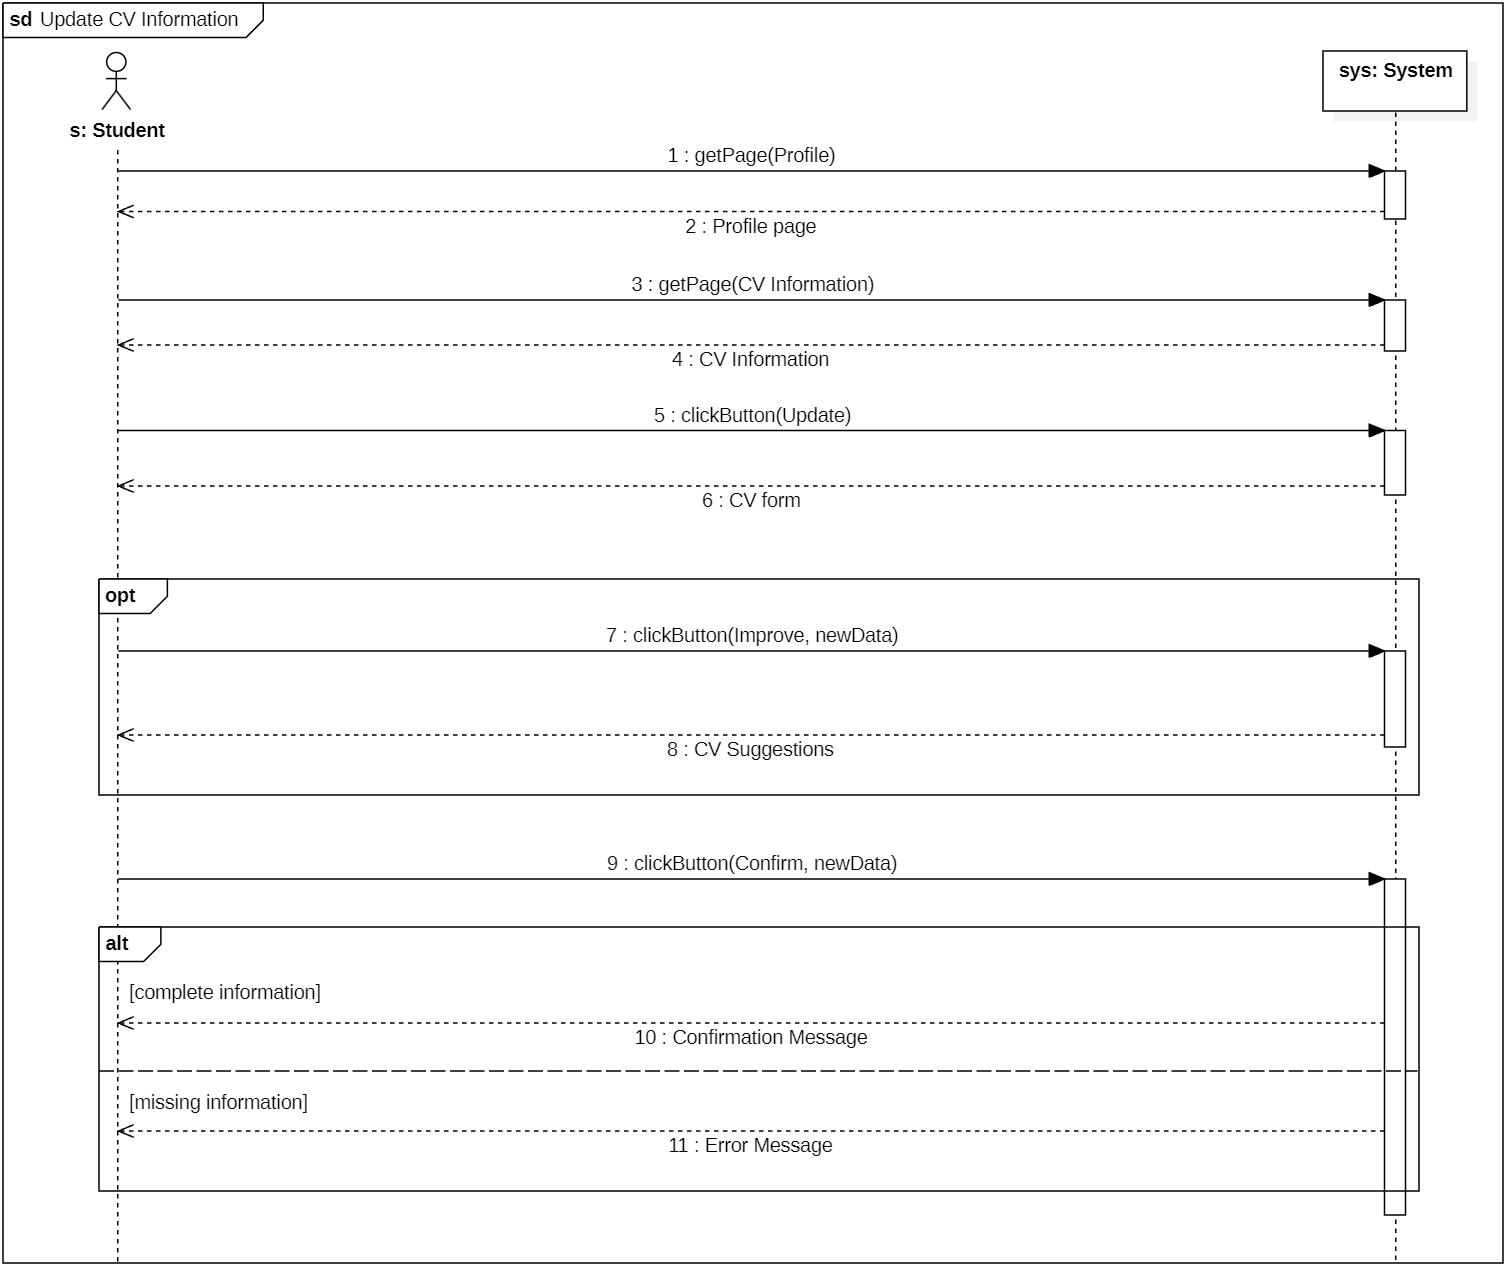
\includegraphics[width=1\linewidth]{Use Cases Images/update_CV_informations.png}
    \caption{Diagram for [UC4]}
    \label{fig: Update CV Information Diagram}
\end{figure}

\subsubsection*{Create Internship}
\begin{table}[H]
    \centering
    \renewcommand{\arraystretch}{1.5}
    \begin{tabular}{|p{4cm}|p{11cm}|}
    \hline
    \rowcolor{bluepoli!40}
    \textbf{[UC5]} & \textbf{Create Internship} \\ \hline \hline
    \textbf{Actors} & Company \\ \hline
    \textbf{Entry Condition} & 
    {\setlength{\leftmargini}{1.1em}
    \begin{itemize}
        \item The company is registered.
        \item The company is logged in.
    \end{itemize}} \\ \hline
    \textbf{Input} & All the necessary information for creating an internship, such as skills needed, pre-requirements, type of job, start and end dates. \\ \hline
    \textbf{Event Flow} & 
    {\setlength{\leftmargini}{1.4em}
    \begin{enumerate}
        \item The company accesses the internship page.
        \item The company clicks on the "Add Internship" button.
        \item The company fills in the sections with the required information (pre-requirements, type of job).
        \item If the company wants, clicks on the "Improve" button.
        \item The system provides suggestions to improve the proposal.
        \item The company makes adjustments based on the suggestions.
        \item The company clicks on the "Save" button.
    \end{enumerate}} \\ \hline
    \textbf{Exit Condition} & 
    {\setlength{\leftmargini}{1.1em}
    \begin{itemize}
        \item The new internship is now visible in the company’s profile and accessible on the platform for application.
    \end{itemize}} \\ \hline
    \textbf{Output} & 
    The company receives a message confirming the creation of the internship. \\ \hline
    \textbf{Exceptions} & 
    \textbf{Missing Information}: If required fields are not completed, the system prompts the company to fill out all mandatory sections. \\ \hline
    \end{tabular}
    \caption{Create Internship Table}
\end{table}

\begin{figure} [H]
    \centering
    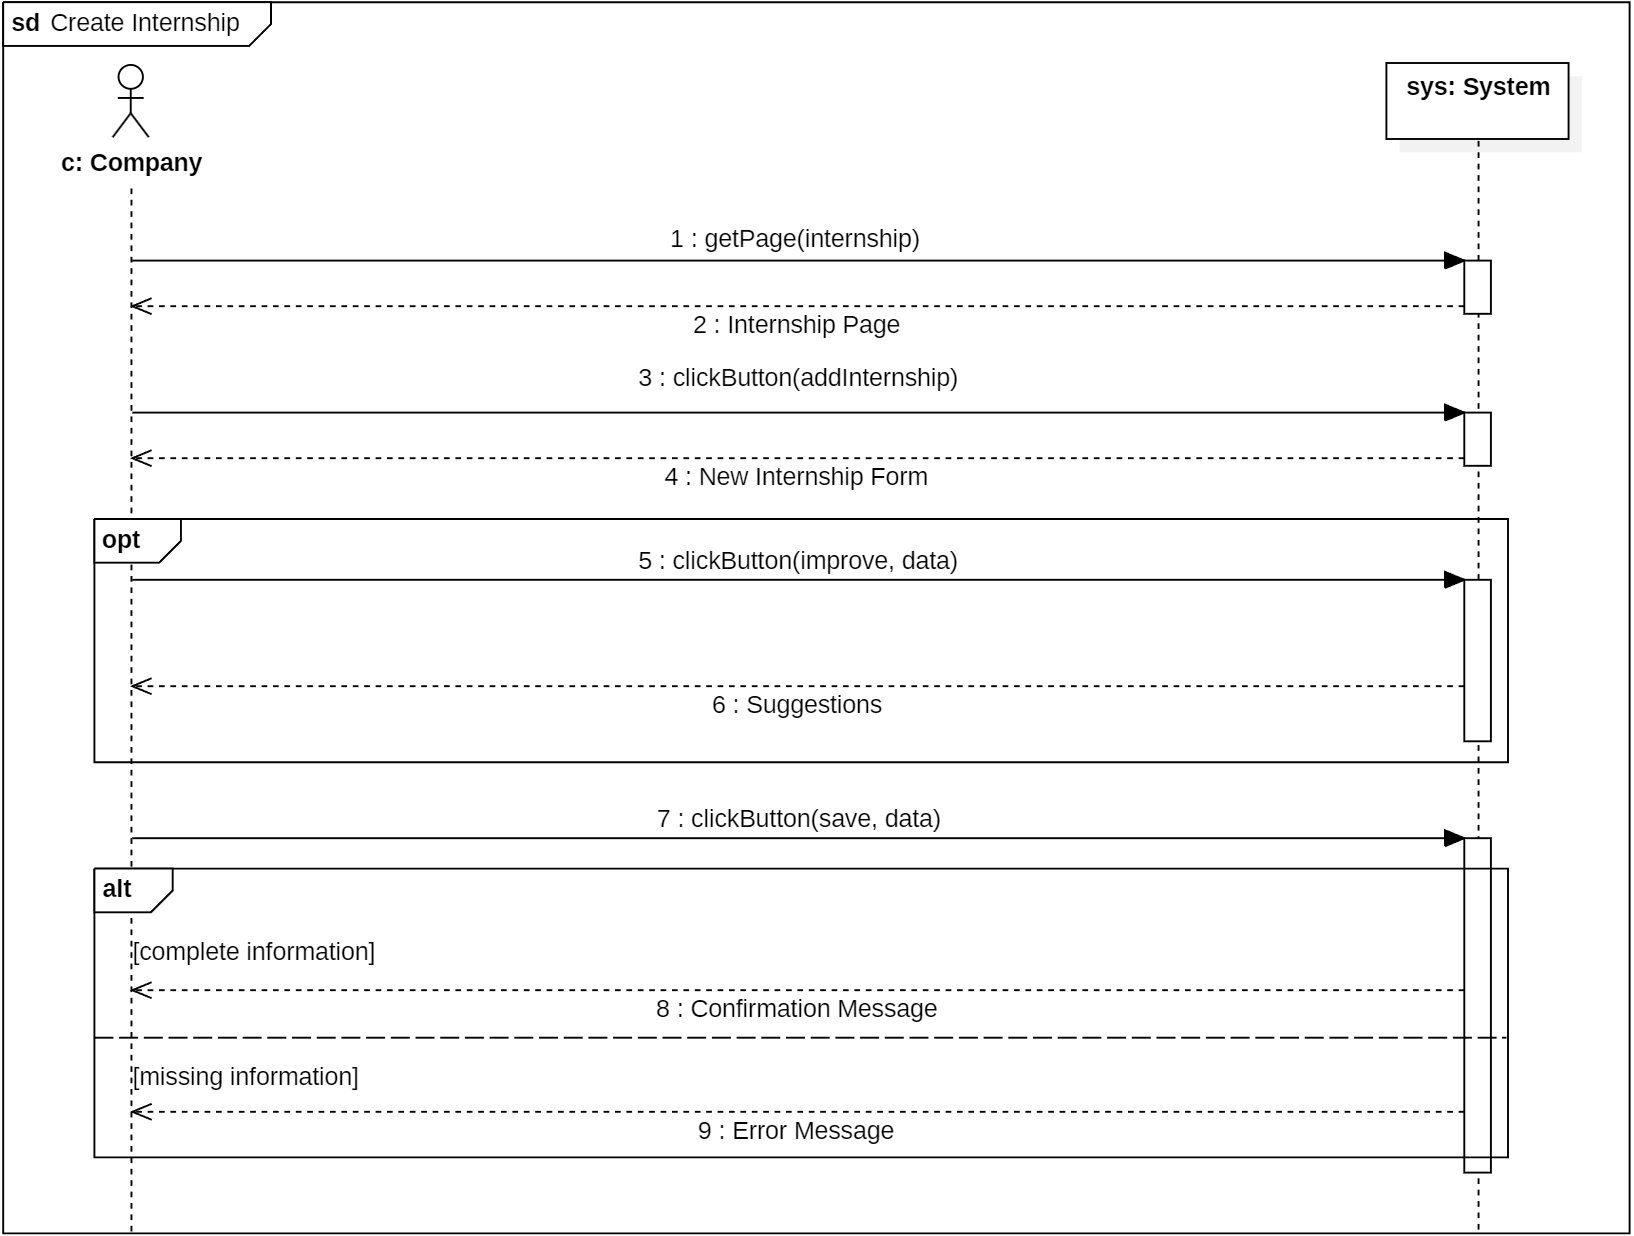
\includegraphics[width=1\linewidth]{Use Cases Images/create_internship.png}
    \caption{Diagram for [UC5]}
    \label{fig: Create Internship Diagram}
\end{figure}

\subsubsection*{Update Internship}
\begin{table}[H]
    \centering
    \renewcommand{\arraystretch}{1.5}
    \begin{tabular}{|p{4cm}|p{11cm}|}
    \hline
    \rowcolor{bluepoli!40}
    \textbf{[UC6]} & \textbf{Update Internship} \\ \hline \hline
    \textbf{Actors} & Company, Student \\ \hline
    \textbf{Entry Condition} & 
    {\setlength{\leftmargini}{1.1em}
    \begin{itemize}
        \item The company is registered.
        \item The company is logged in.
        \item The company has already created the internship.
        \item End date for application is not already expired.
    \end{itemize}} \\ \hline
    \textbf{Input} & Updated internship information such as skills needed, pre-requirements, type of job, start and end dates. \\ \hline
    \textbf{Event Flow} & 
    {\setlength{\leftmargini}{1.4em}
    \begin{enumerate}
        \item The company accesses its profile page.
        \item The company navigates to the "Internship" section.
        \item The company clicks on the "Edit Internship" button.
        \item The company updates the relevant sections of the internship (e.g., modifies dates, location, or pre-requirements).
        \item The company clicks "Save" to confirm the changes.
        \item The system notifies all students that already submitted the application about the changes.
    \end{enumerate}} \\ \hline
    \textbf{Exit Condition} & 
    {\setlength{\leftmargini}{1.1em}
    \begin{itemize}
        \item The updated internship is now visible in the company's profile.
    \end{itemize}} \\ \hline
    \textbf{Output} & 
    {\setlength{\leftmargini}{1.1em}
    \begin{itemize}
        \item A confirmation message is displayed to the company indicating that the internship has been successfully updated.
        \item The students that already submitted the application for it are notified about the changes.
    \end{itemize}} \\ \hline
    \textbf{Exceptions} & 
    \textbf{Missing Information}: If required fields are not completed, the system prompts the company to fill out all mandatory sections. \\ \hline
    \end{tabular}
    \caption{Update Internship Table}
\end{table}

\begin{figure} [H]
    \centering
    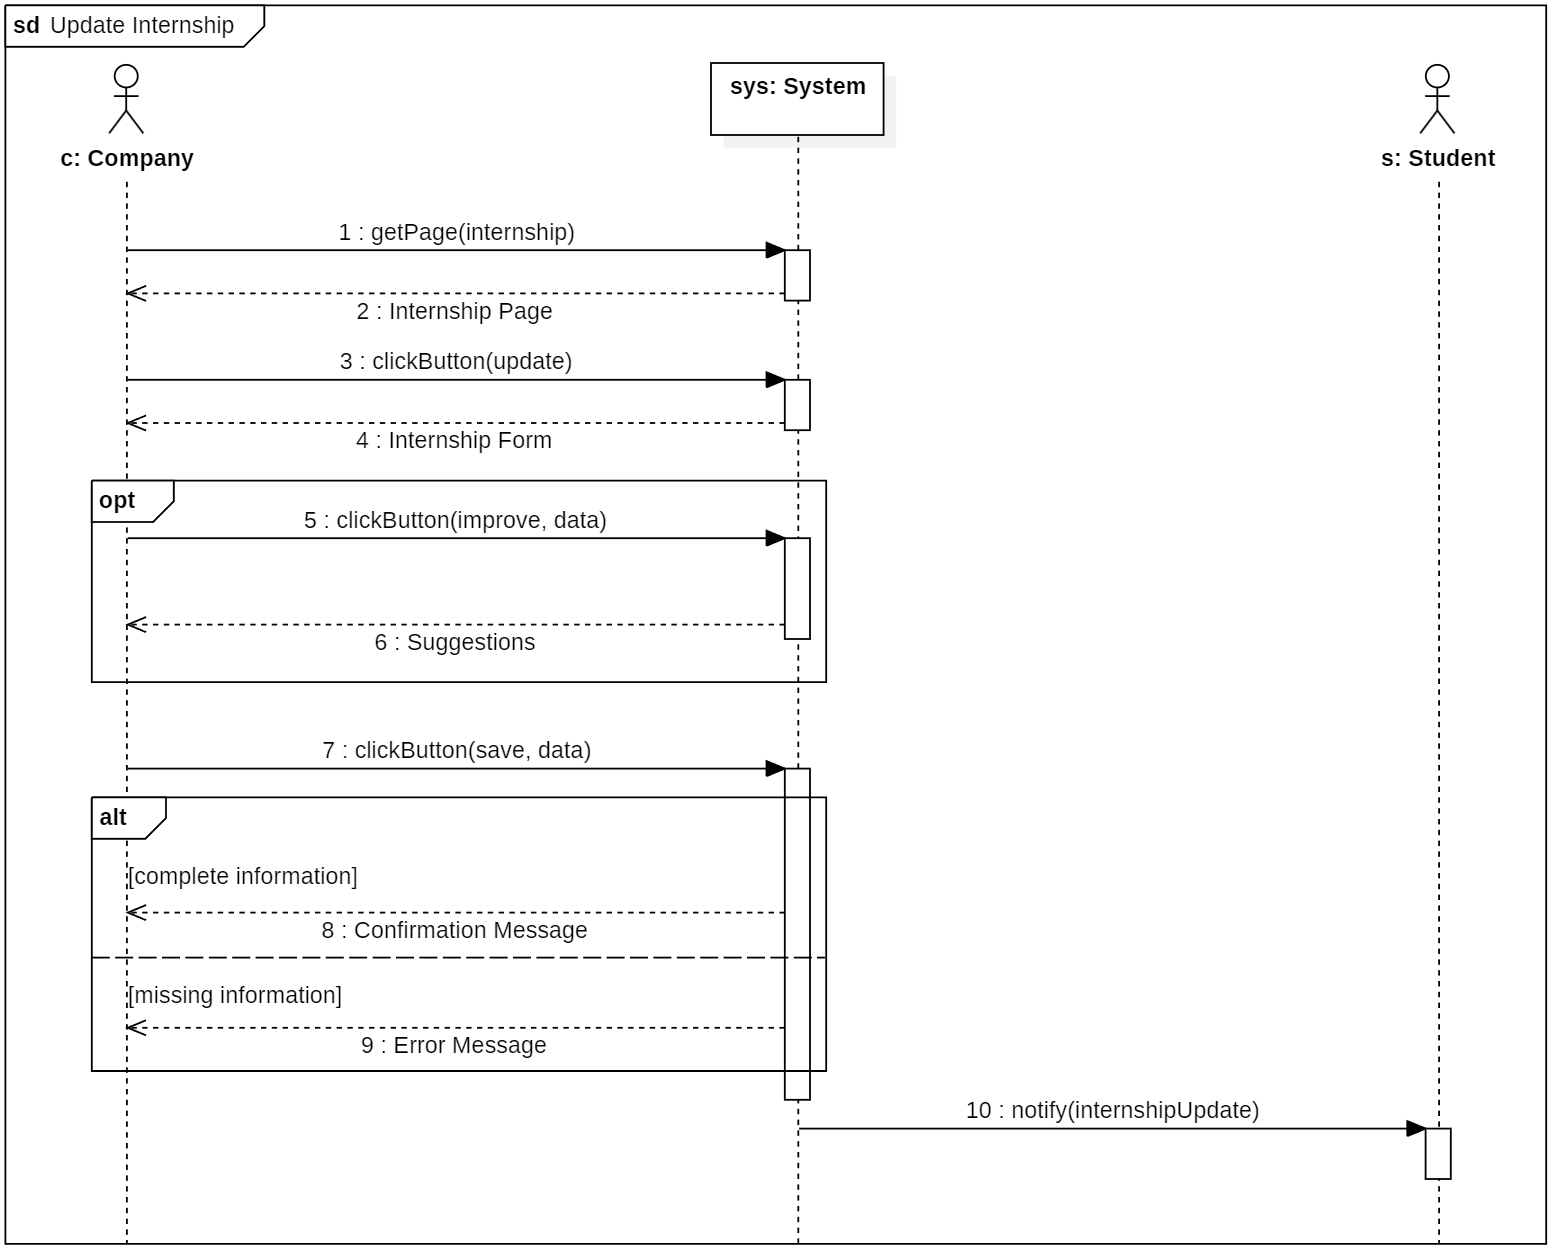
\includegraphics[width=1\linewidth]{Use Cases Images/update_internship.png}
    \caption{Diagram for [UC6]}
    \label{fig: Update Internship Diagram}
\end{figure}

\subsubsection*{Search Internship}
\begin{table}[H]
    \centering
    \renewcommand{\arraystretch}{1.5}
    \begin{tabular}{|p{4cm}|p{11cm}|}
    \hline
    \rowcolor{bluepoli!40}
    \textbf{[UC7]} & \textbf{Search Internship} \\ \hline \hline
    \textbf{Actors} & Student \\ \hline
    \textbf{Entry Condition} & 
    {\setlength{\leftmargini}{1.1em}
    \begin{itemize}
        \item The student has registered.
        \item The student is logged in.
    \end{itemize}} \\ \hline
    \textbf{Input} & 
    {\setlength{\leftmargini}{1.1em}
    \begin{itemize}
        \item Search criteria such as preferred location, required skills, duration, and type of internship.
        \item Keywords related to specific interests or roles the student wants to explore.
    \end{itemize}} \\ \hline
    \textbf{Event Flow} & 
    {\setlength{\leftmargini}{1.4em}
    \begin{enumerate}
        \item The student navigates to the internship page.
        \item The student enters search criteria, such as location, industry type, and duration, or uses keywords to find specific roles of interest.
        \item The student clicks on the "Search" button.
        \item The system displays a list of internships that match the student's search criteria.
    \end{enumerate}} \\ \hline
    \textbf{Exit Condition} & 
    {\setlength{\leftmargini}{1.1em}
    \begin{itemize}
        \item The student receives a list of internships that match their search criteria or recommendations from the system.
    \end{itemize}} \\ \hline
    \textbf{Output} & 
    A list of internships matching the student’s search criteria and system recommendations are displayed to the student. \\ \hline
    \textbf{Exceptions} & 
    {\setlength{\leftmargini}{1.1em}
    \begin{itemize}
        \item \textbf{No Matching Internships}: If no internships match the student's criteria, the system displays a message indicating that there are no available opportunities and suggests changing the search criteria.
    \end{itemize}} \\ \hline
    \end{tabular}
    \caption{Search Internship Table}
\end{table}

\begin{figure} [H]
    \centering
    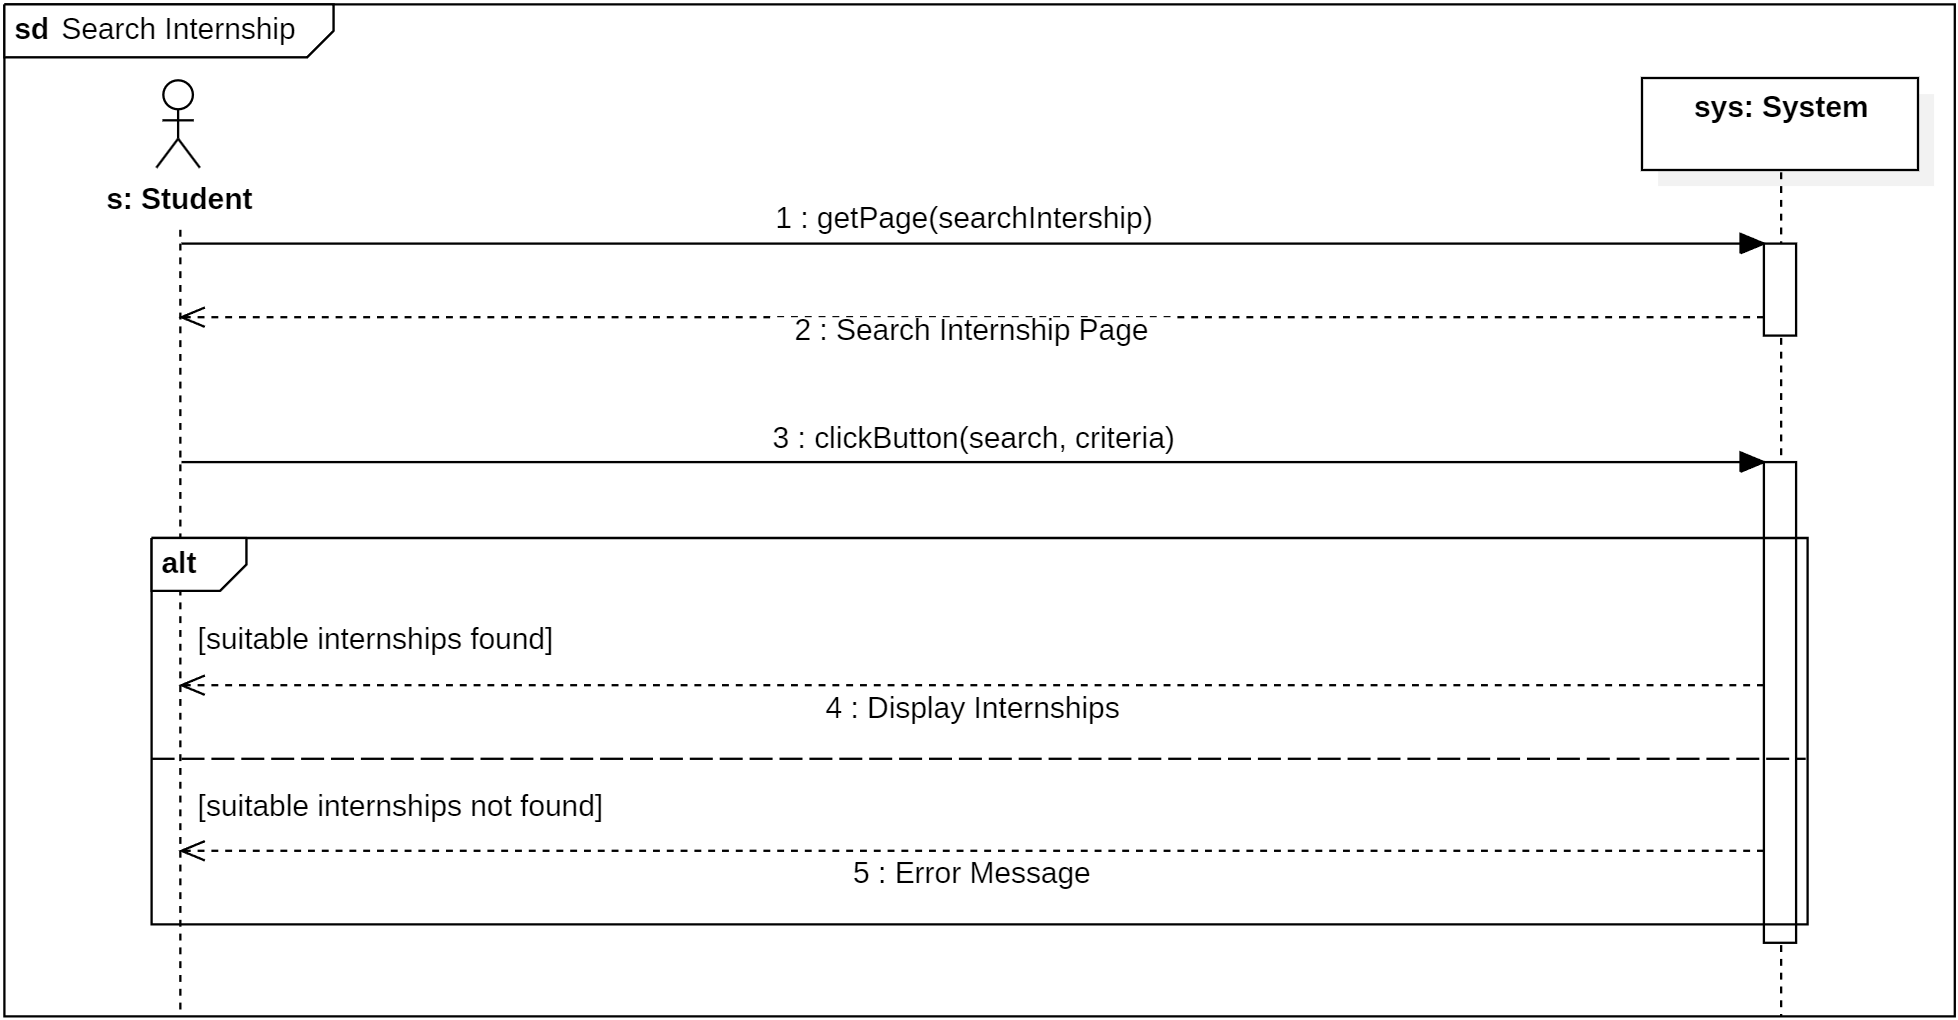
\includegraphics[width=1\linewidth]{Use Cases Images/search_internship.png}
    \caption{Diagram for [UC7]}
    \label{fig: Search Internship Diagram}
\end{figure}

\subsubsection*{Submit Application}

\begin{table}[H]
    \centering
    \renewcommand{\arraystretch}{1.5}
    \begin{tabular}{|p{4cm}|p{11cm}|}
    \hline
    \rowcolor{bluepoli!40}
    \textbf{[UC8]} & \textbf{Submit Application} \\ \hline \hline
    \textbf{Actors} & Student \\ \hline
    \textbf{Entry Condition} & 
    {\setlength{\leftmargini}{1.1em}
    \begin{itemize}
        \item The student has registered.
        \item The student is logged in.
        \item The student has completed their profile with the CV information.
    \end{itemize}} \\ \hline
    \textbf{Input} & Information for the internship (such as motivational letter, etc.). \\ \hline
    \textbf{Event Flow} & 
    {\setlength{\leftmargini}{1.4em}
    \begin{enumerate}
        \item The student select the internship they want to apply for.
        \item The student clicks on the "Apply" button.
        \item The student fills out the form for the application.
        \item The student click on the "Submit" button.
        \item The system saves the application and notifies the company.
    \end{enumerate}} \\ \hline
    \textbf{Exit Condition} & 
    {\setlength{\leftmargini}{1.1em}
    \begin{itemize}
        \item The application is successfully submitted.
    \end{itemize}} \\ \hline
    \textbf{Output} & 
    The student is notified of the successful submission. \\ \hline
    \textbf{Exceptions} & 
    {\setlength{\leftmargini}{1.1em}
    \begin{itemize}
        \item \textbf{Missing Requirements:} If the student does not satisfy the requirements of the internship, an exception is raised.
        \item \textbf{Incomplete Application:} If the application contains missing or incomplete information, the system highlights the missing parts and suggests to the student the mandatory sections to complete.
    \end{itemize}} \\ \hline
    \end{tabular}
    \caption{Submit Application Table}
\end{table}

\begin{figure} [H]
    \centering
    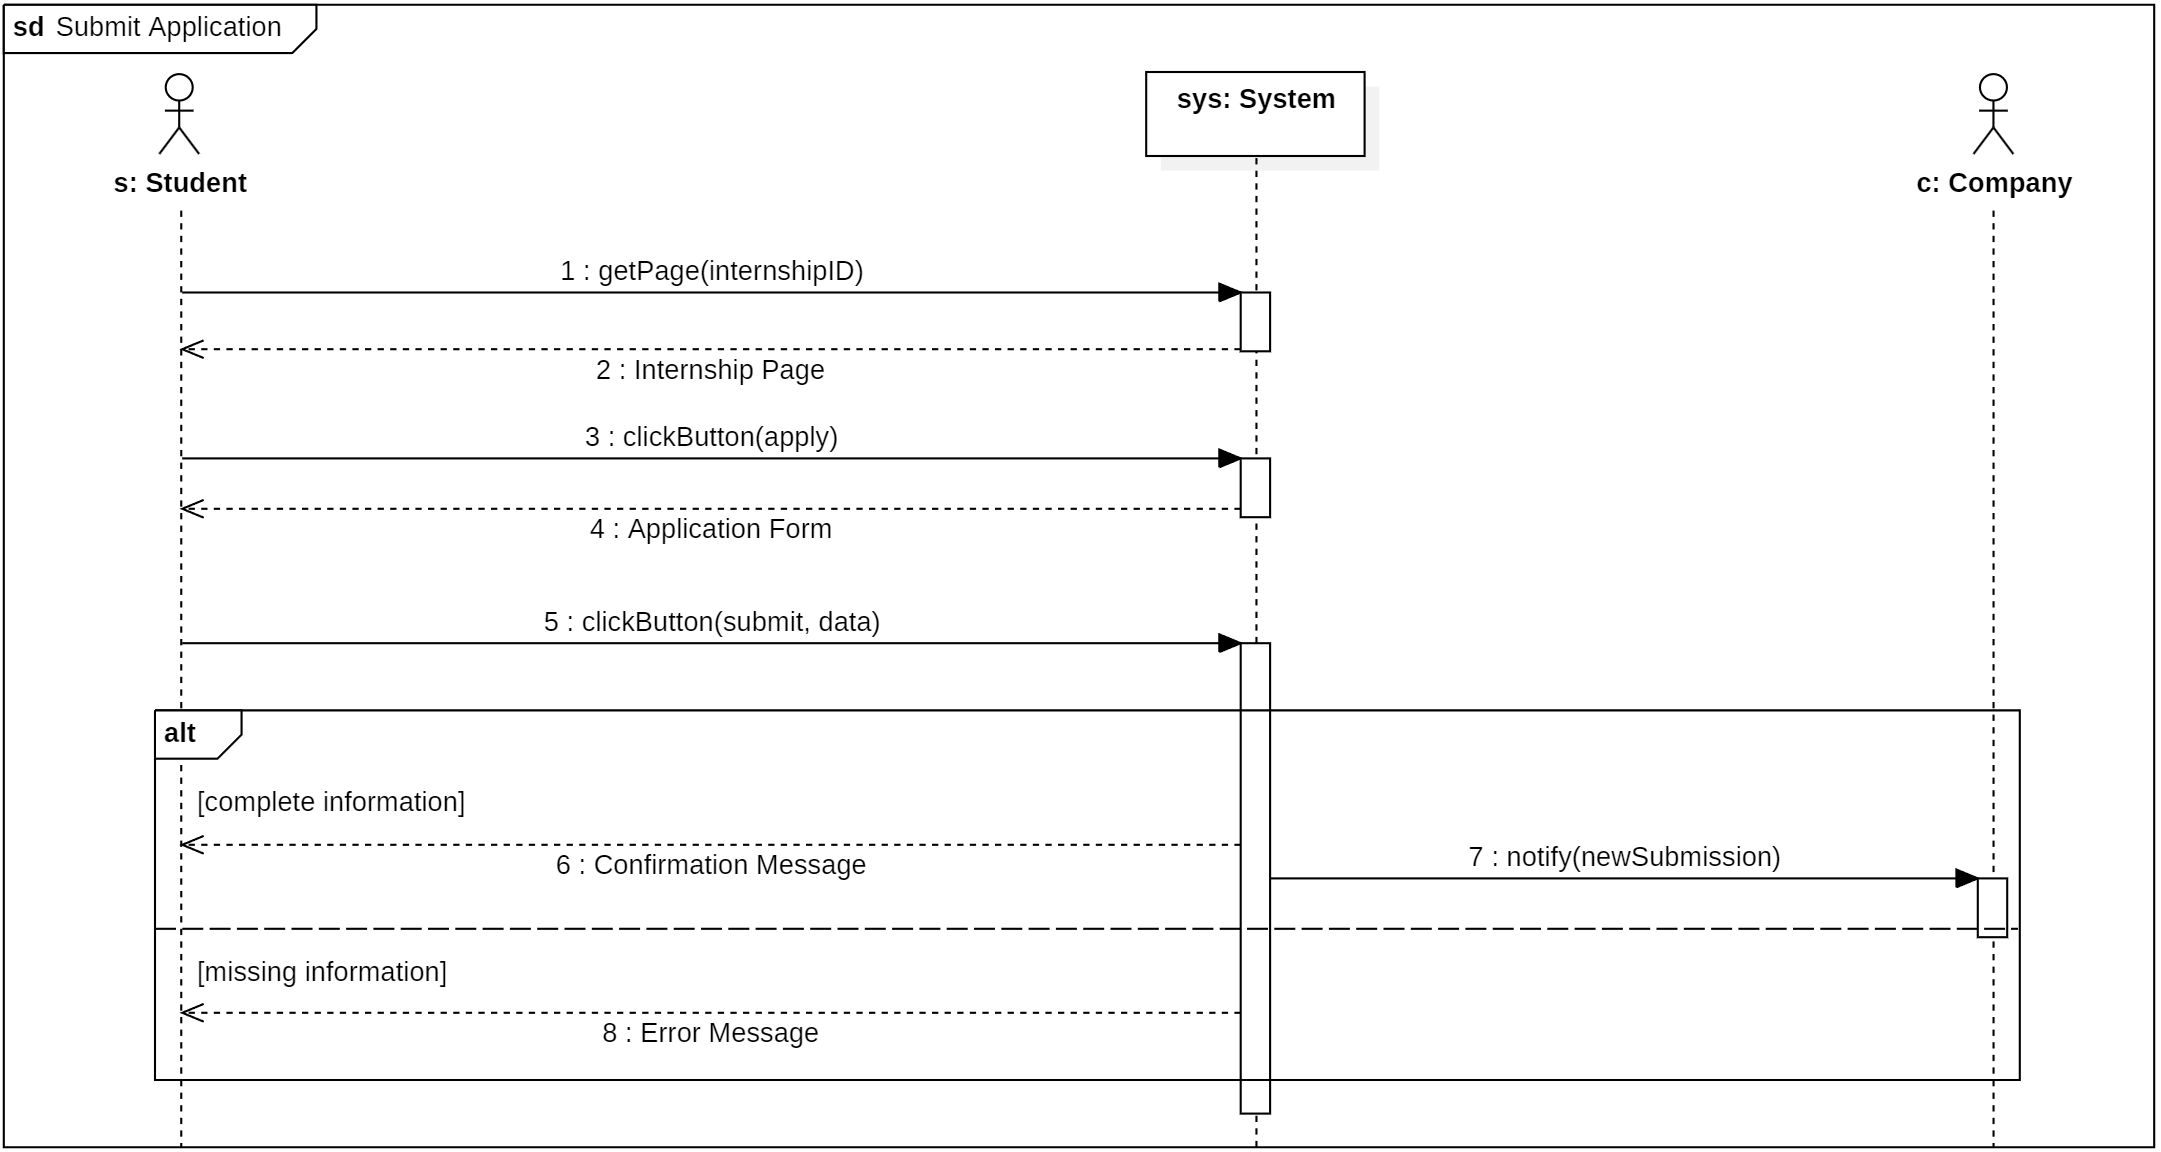
\includegraphics[width=1\linewidth]{Use Cases Images/submit_application.png}
    \caption{Diagram for [UC8]}
    \label{fig: Submit Application Diagram}
\end{figure}


\subsubsection*{Insert Questionnaire}
\begin{table}[H]
    \centering
    \renewcommand{\arraystretch}{1.5}
    \begin{tabular}{|p{4cm}|p{11cm}|}
    \hline
    \rowcolor{bluepoli!40}
    \textbf{[UC9]} & \textbf{Insert Questionnaire} \\ \hline \hline
    \textbf{Actors} & Company, Student \\ \hline
    \textbf{Entry Condition} & 
    \begin{itemize}
        \item The company is registered.
        \item The company is logged in.
        \item Time for internship application is expired.
    \end{itemize} \\ \hline
    \textbf{Input} & 
    All necessary questions to understand the skills and requirements of the candidates. \\ \hline
    \textbf{Event Flow} & 
    {\setlength{\leftmargini}{1.4em}
    \begin{enumerate}
        \item The company accesses the internship page.
        \item The company clicks on the "Insert New Questionnaire" button.
        \item The company fills in the sections with the necessary questions.
        \item If the company wants, clicks on the "Improve" button.
        \item The system provides suggestions to improve the quality of questions.
        \item The company makes adjustments based on the suggestions.
        \item The company clicks on the "Save" button.
        \item The system notifies all students who submitted the application about the availability of the questionnaire.
    \end{enumerate}} \\ \hline
    \textbf{Exit Condition} & 
    The new questionnaire is now visible in the internship section. \\ \hline
    \textbf{Output} & 
    {\setlength{\leftmargini}{1.1em}
    \begin{itemize}
        \item A confirmation message is displayed to the company indicating that the questionnaire has been successfully uploaded.
        \item The students who submitted the application for it are notified about the availability of the questionnaire.
    \end{itemize}} \\ \hline
    \textbf{Exceptions} & 
    \textbf{Missing Information}: If required fields are not completed, the system prompts the company to fill out all mandatory sections. \\ \hline
    \end{tabular}
    \caption{Insert Questionnaire Table}
\end{table}

\begin{figure} [H]
    \centering
    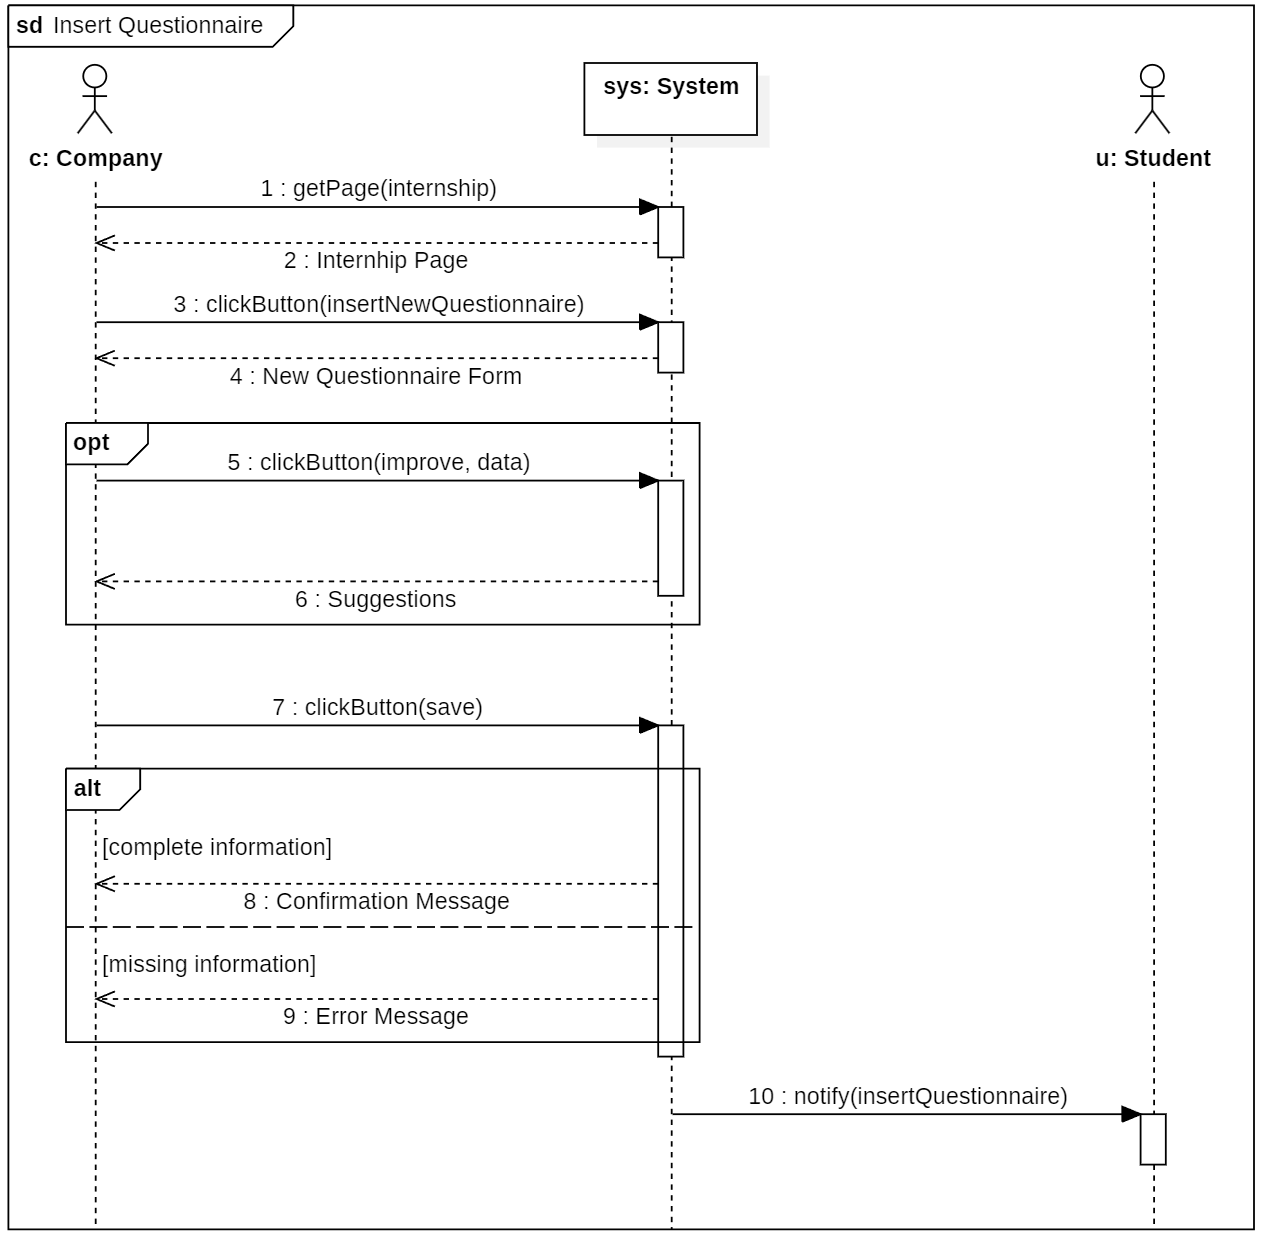
\includegraphics[width=1\linewidth]{Use Cases Images/insert_questionnaire.png}
    \caption{Diagram for [UC9]}
    \label{fig: Insert Questionnaire Diagram}
\end{figure}


\subsubsection*{Update Questionnaire}
\begin{table}[H]
    \centering
    \renewcommand{\arraystretch}{1.5}
    \begin{tabular}{|p{4cm}|p{11cm}|}
    \hline
    \rowcolor{bluepoli!40}
    \textbf{[UC10]} & \textbf{Update Questionnaire} \\ \hline \hline
    \textbf{Actors} & Company, Student \\ \hline
    \textbf{Entry Condition} & 
    {\setlength{\leftmargini}{1.1em}
    \begin{itemize}
        \item The company is registered.
        \item The company is logged in.
        \item Questionnaire is already live on the platform.
    \end{itemize}} \\ \hline
    \textbf{Input} & 
    All necessary questions to update to understand the skills and requirements of the candidates. \\ \hline
    \textbf{Event Flow} & 
    {\setlength{\leftmargini}{1.4em}
    \begin{enumerate}
        \item The company accesses the internship page.
        \item The company clicks on the "Update" button.
        \item The company fills in the sections with the necessary questions.
        \item If the company wants, clicks on the "Improve" button.
        \item The system provides suggestions to improve the quality of questions.
        \item The company makes adjustments based on the suggestions.
        \item The company clicks on the "Save" button.
        \item The system notifies all students who submitted the application about the changes to the questionnaire.
    \end{enumerate}} \\ \hline
    \textbf{Exit Condition} & 
    The updated questionnaire is now visible in the internship section. \\ \hline
    \textbf{Output} & 
    {\setlength{\leftmargini}{1.1em}
    \begin{itemize}
        \item A confirmation message is displayed to the company indicating that the questionnaire has been successfully updated.
        \item The students who submitted the application for it are notified about the changes to the questionnaire.
    \end{itemize}} \\ \hline
    \textbf{Exceptions} & 
    \textbf{Missing Information}: If required fields are not completed, the system prompts the company to fill out all mandatory sections. \\ \hline
    \end{tabular}
    \caption{Update Questionnaire Table}
\end{table}

\begin{figure} [H]
    \centering
    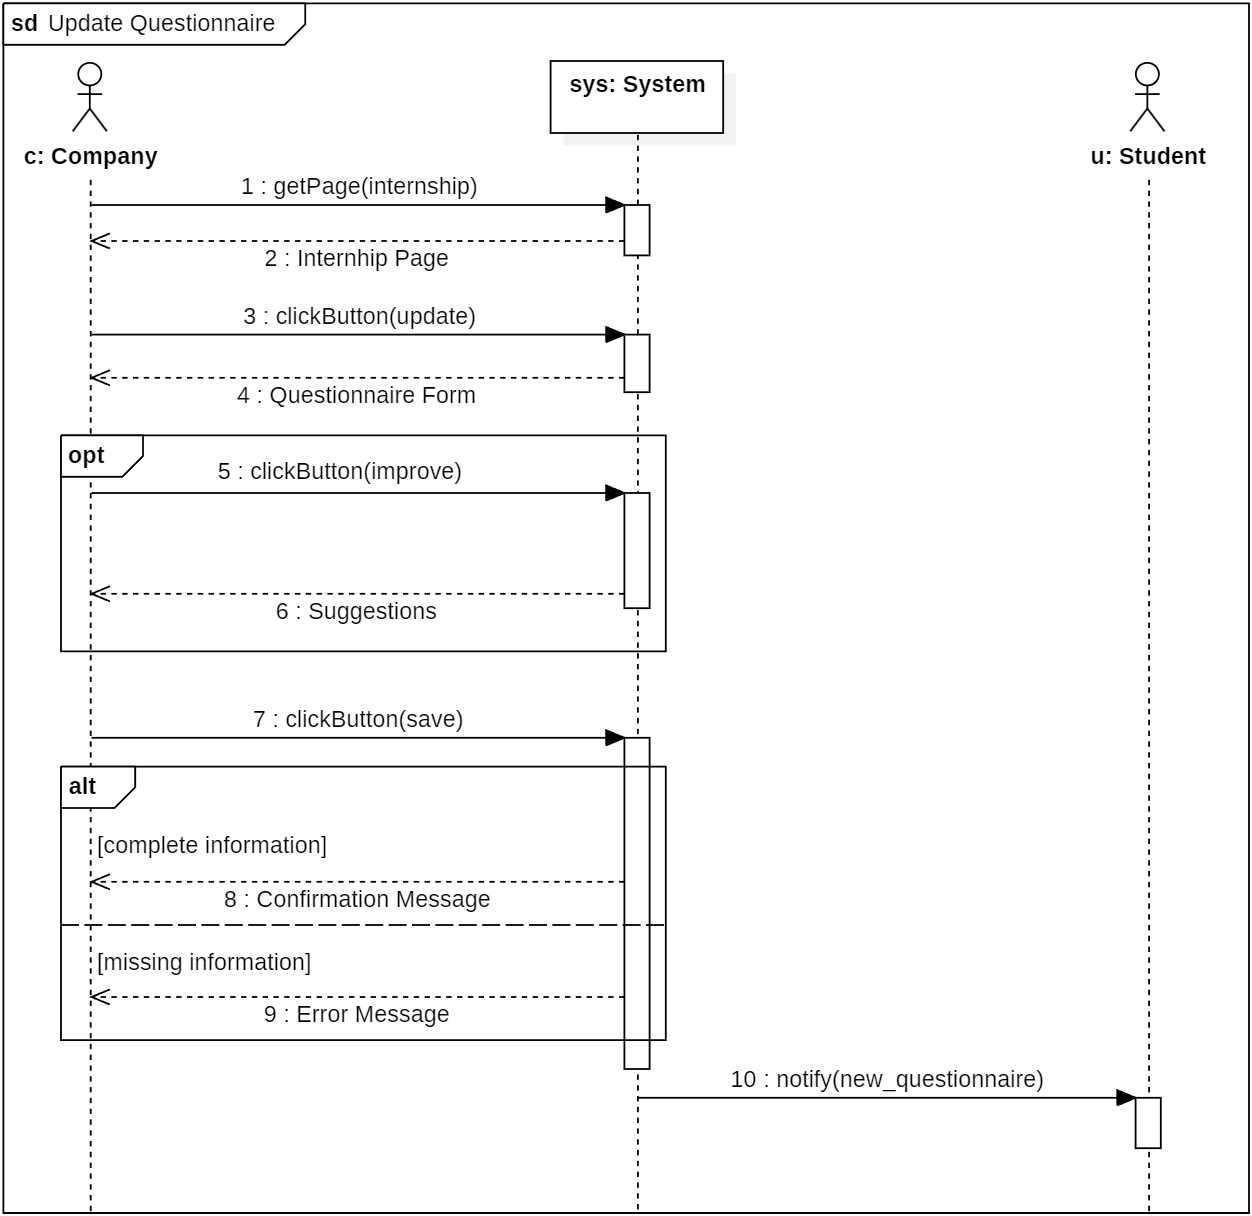
\includegraphics[width=1\linewidth]{Use Cases Images/update_questionnaire.png}
    \caption{Diagram for [UC10]}
    \label{fig: Update Questionnaire Diagram}
\end{figure}


\subsubsection*{Answer Questionnaire}
\begin{table}[H]
    \centering
    \renewcommand{\arraystretch}{1.5}
    \begin{tabular}{|p{4cm}|p{11cm}|}
    \hline
    \rowcolor{bluepoli!40}
    \textbf{[UC11]} & \textbf{Answer Questionnaire} \\ \hline \hline
    \textbf{Actors} & Student, Company \\ \hline
    \textbf{Entry Condition} & 
    {\setlength{\leftmargini}{1.1em}
    \begin{itemize}
        \item The student is registered.
        \item The student is logged in.
        \item The student must have received a positive evaluation from the company.
        \item The company must have posted the questionnaire.
    \end{itemize}} \\ \hline
    \textbf{Input} & Answers to the questionnaire. \\ \hline
    \textbf{Event Flow} & 
    {\setlength{\leftmargini}{1.4em}
    \begin{enumerate}
        \item The student navigates to the internship page.
        \item The system shows the list of internships for which the student applied.
        \item The student clicks on the specific internship they are interested in.
        \item The student clicks on the "Answer Questionnaire" button.
        \item The student answers all the questions in the questionnaire.
        \item The student clicks on the "Submit" button.
        \item The system saves the form and notifies the company.
    \end{enumerate}} \\ \hline
    \textbf{Exit Condition} & 
    {\setlength{\leftmargini}{1.1em}
    \begin{itemize}
        \item The questionnaire has been fully answered.
        \item The questionnaire has been successfully submitted.
    \end{itemize}} \\ \hline
    \textbf{Output} & 
    Confirmation message to the student that the questionnaire has been fully answered and sent to the company. \\ \hline
    \textbf{Exceptions} &
    {\setlength{\leftmargini}{1.1em}
    \begin{itemize}
        \item \textbf{Incomplete Information:} If required fields are missing, the system prompts the student to complete all mandatory sections.
    \end{itemize}} \\ \hline
    \end{tabular}
    \caption{Answer Questionnaire Table}
\end{table}

\begin{figure} [H]
    \centering
    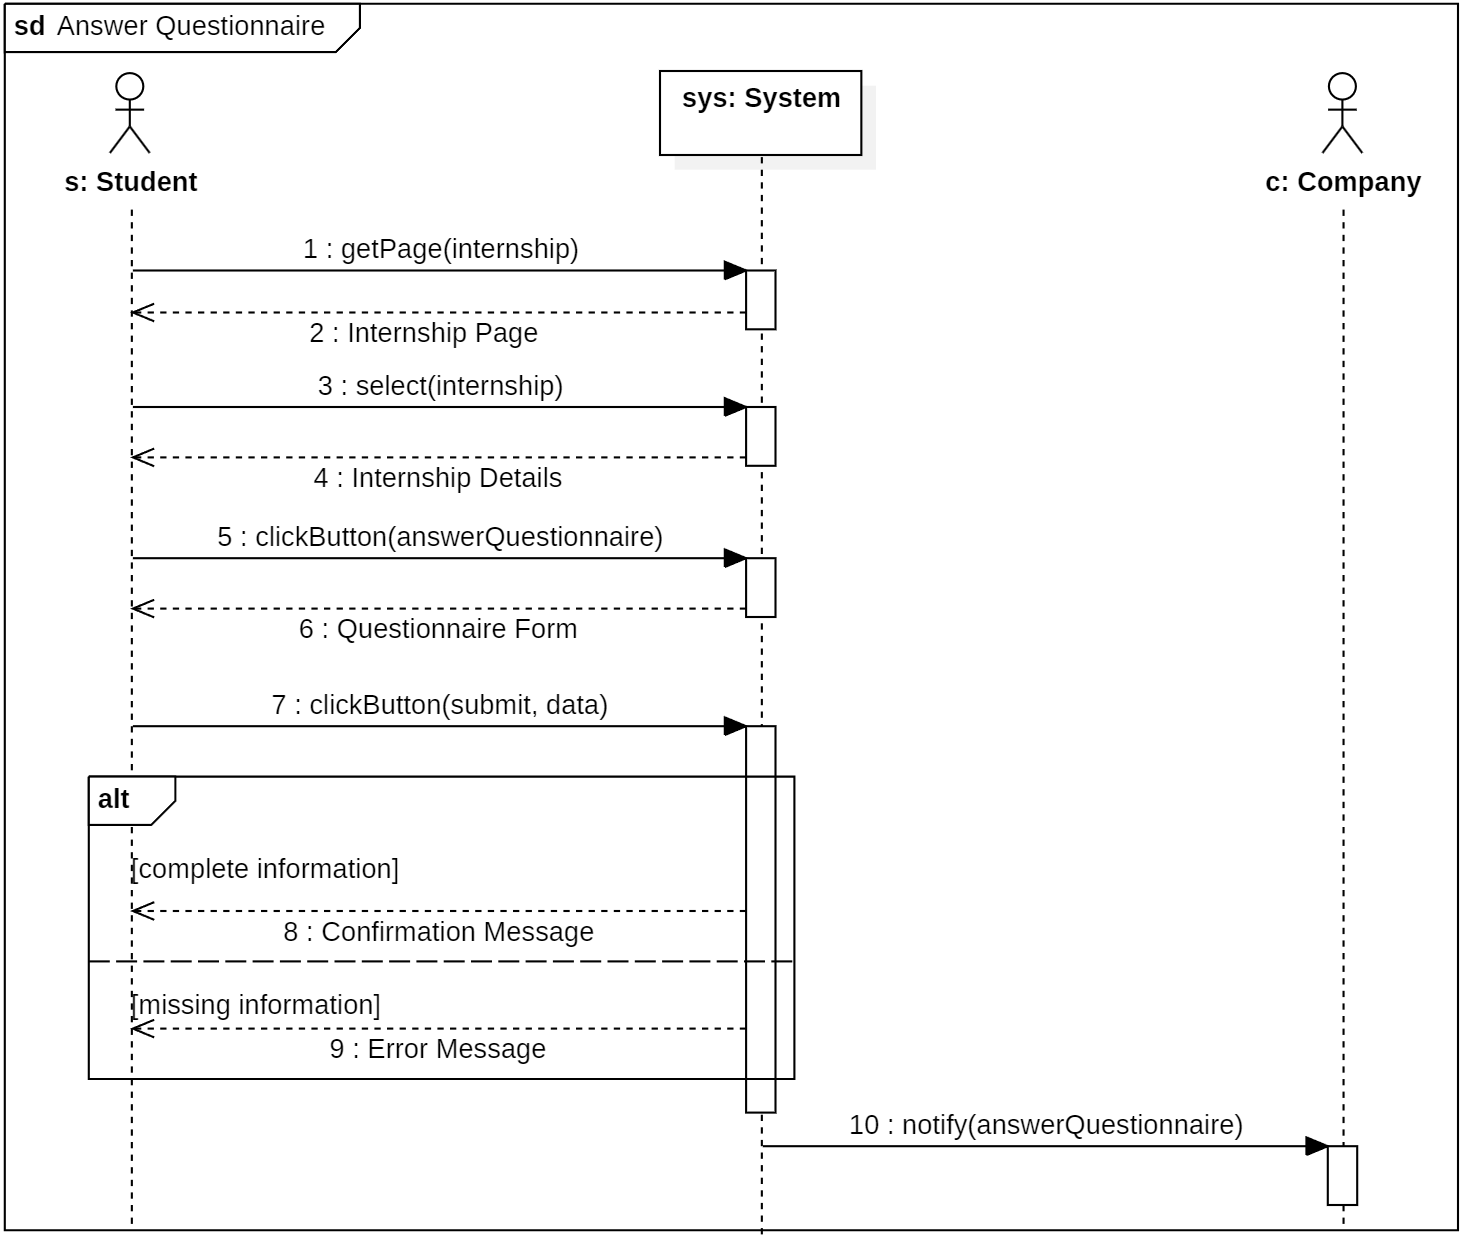
\includegraphics[width=1\linewidth]{Use Cases Images/answer_questionnaire.png}
    \caption{Diagram for [UC11]}
    \label{fig: Answer Questionnaire Diagram}
\end{figure}


\subsubsection*{Evaluate Application}
\begin{table}[H]
    \centering
    \renewcommand{\arraystretch}{1.5}
    \begin{tabular}{|p{4cm}|p{11cm}|}
    \hline
    \rowcolor{bluepoli!40}
    \textbf{[UC12]} & \textbf{Evaluate Applications} \\ \hline \hline
    \textbf{Actors} & Company, Student \\ \hline
    \textbf{Entry Condition} & 
    {\setlength{\leftmargini}{1.1em}
    \begin{itemize}
        \item The company is registered on the platform.
        \item The company is logged in.
        \item The company has already posted an internship position.
    \end{itemize}} \\ \hline
    \textbf{Input} & / \\ \hline
    \textbf{Event Flow} & 
    {\setlength{\leftmargini}{1.4em}
    \begin{enumerate}
        \item The company navigates to the internship page.
        \item The company selects the internship for which it wants to evaluate the applications.
        \item The system shows the list of applications received for the internship.
        \item The company selects an application to review the candidate details.
        \item The system displays the candidate's profile, CV, and other submitted documents.
        \item The company clicks on the "Manage" button.
        \item The company decides whether to reject the application, schedule an interview or to shortlist the candidate.
        \item The company clicks on the "Save" button.
        \item The students are notified with the decision of the company.
    \end{enumerate}} \\ \hline
    \textbf{Exit Condition} & 
    {\setlength{\leftmargini}{1.1em}
    \begin{itemize}
        \item The internship application status is updated.
        \item The students are notified.
    \end{itemize}} \\ \hline
    \textbf{Output} & 
    For each application, the new status is shown (e.g., “rejected,” “pending interview,” etc.). \\ \hline
    \textbf{Exceptions} & 
    {\setlength{\leftmargini}{1.1em}
    \begin{itemize}
        \item \textbf{No Applications Available:} If no applications are available, the system displays a message indicating that there are no applications to evaluate.
    \end{itemize}} \\ \hline
    \end{tabular}
    \caption{Evaluate Application Table}
\end{table}

\begin{figure} [H]
    \centering
    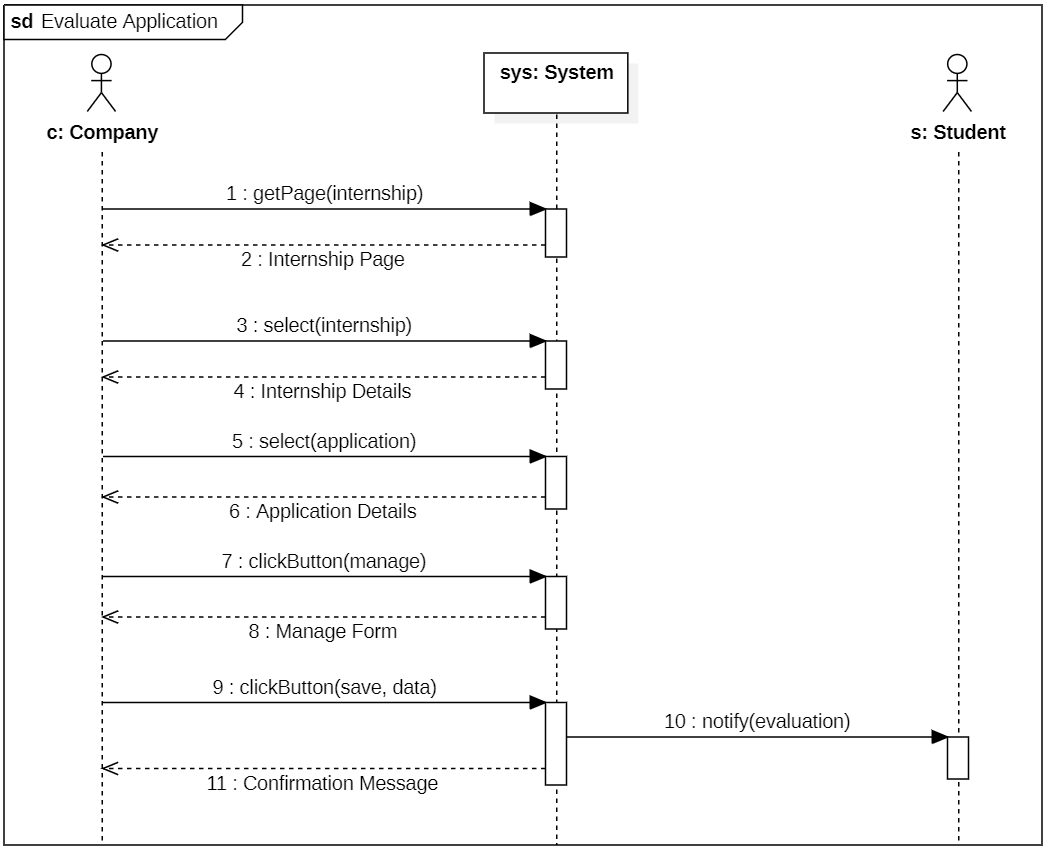
\includegraphics[width=1\linewidth]{Use Cases Images/evaluate application.png}
    \caption{Diagram for [UC12]}
    \label{fig: Evaluate Application Diagram}
\end{figure}

\subsubsection*{Monitor Internship}
\begin{table}[H]
    \centering
    \renewcommand{\arraystretch}{1.5}
    \begin{tabular}{|p{4cm}|p{11cm}|}
    \hline
    \rowcolor{bluepoli!40}
    \textbf{[UC13]} & \textbf{Monitor Internship} \\ \hline \hline
    \textbf{Actors} & User \\ \hline
    \textbf{Entry Condition} & 
    {\setlength{\leftmargini}{1.1em}
    \begin{itemize}
        \item The user has registered.
        \item The user is logged in.
        \item The student has applied for an internship.
    \end{itemize}} \\ \hline
    \textbf{Input} & / \\ \hline
    \textbf{Event Flow} & 
    {\setlength{\leftmargini}{1.4em}
    \begin{enumerate}
        \item The user navigates to the internship page.
        \item The system shows the list of internships for which the student applied.
        \item The student selects the specific internship they are interested in.
        \item The system displays all the information regarding the internship.
    \end{enumerate}} \\ \hline
    \textbf{Exit Condition} & 
    {\setlength{\leftmargini}{1.1em}
    \begin{itemize}
        \item The student visualizes the information they are interested in.
    \end{itemize}} \\ \hline
    \textbf{Output} & 
    The information are displayed.\\ \hline
    \textbf{Exceptions} & / \\ \hline
    \end{tabular}
    \caption{Monitor Internship Table}
\end{table}

\begin{figure} [H]
    \centering
    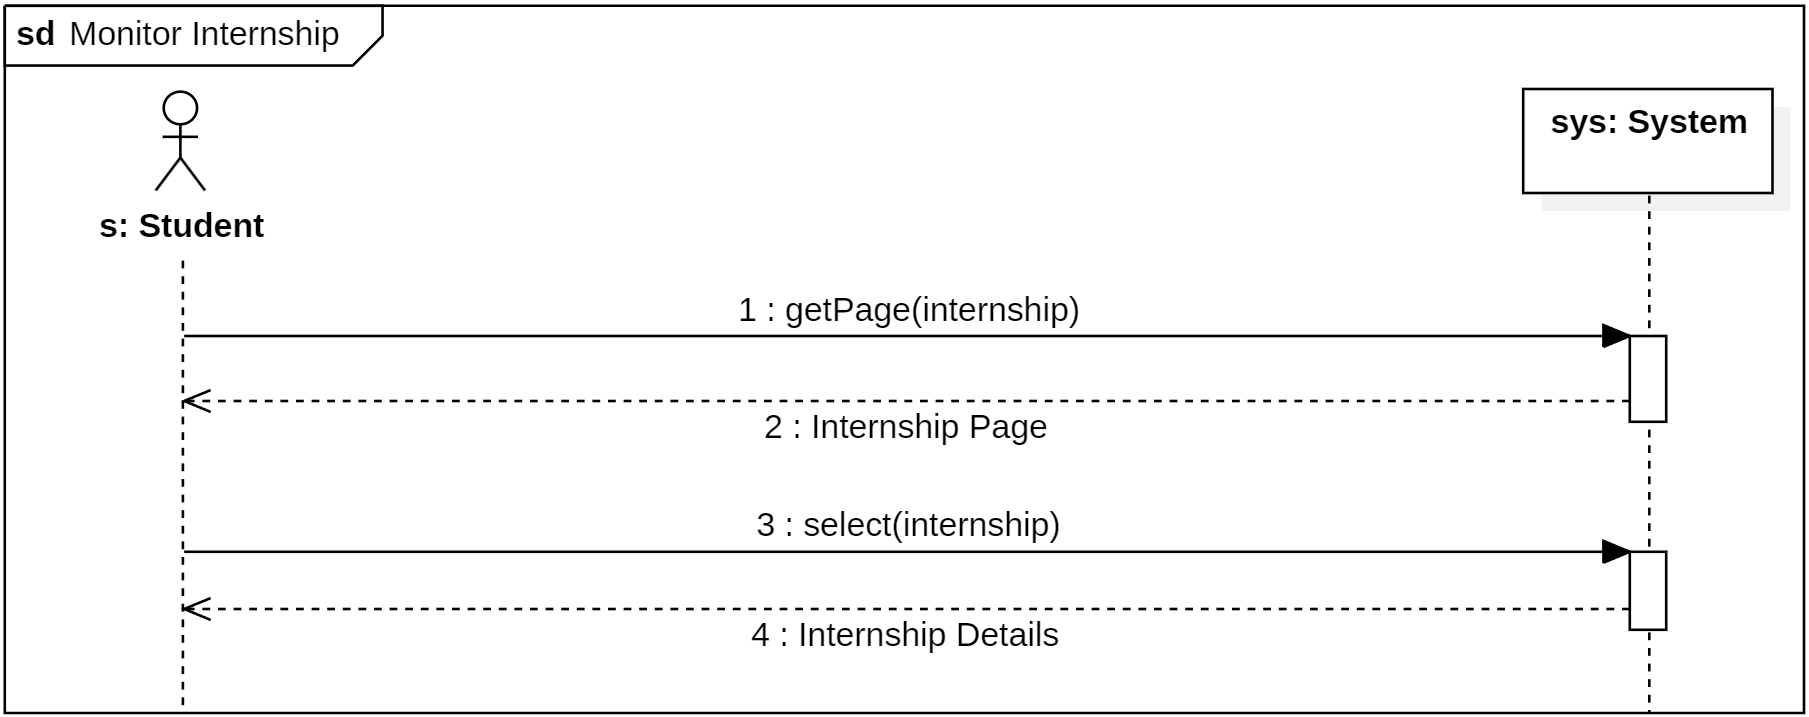
\includegraphics[width=1\linewidth]{Use Cases Images/monitor_internship.png}
    \caption{Diagram for [UC13]}
    \label{fig: Monitor Internship Diagram}
\end{figure}

\subsubsection*{Write feedback}
\begin{table}[H]
    \centering
    \renewcommand{\arraystretch}{1.5}
    \begin{tabular}{|p{4cm}|p{11cm}|}
    \hline
    \rowcolor{bluepoli!40}
    \textbf{[UC14]} & \textbf{Write Feedback} \\ \hline \hline
    \textbf{Actors} & User \\ \hline
    \textbf{Entry Condition} & 
    {\setlength{\leftmargini}{1.1em}
    \begin{itemize}
        \item The user has registered.
        \item The user is logged in.
    \end{itemize}} \\ \hline
    \textbf{Input} & Information about the problem to report. \\ \hline
    \textbf{Event Flow} & 
    {\setlength{\leftmargini}{1.4em}
    \begin{enumerate}
        \item The user navigates to the home page.
        \item The user clicks on the "Write Feedback" button.
        \item The user fills out the form for the feedback.
        \item The user clicks on the "Send" button.
    \end{enumerate}} \\ \hline
    \textbf{Exit Condition} & 
    {\setlength{\leftmargini}{1.1em}
    \begin{itemize}
        \item The feedback is sent.
    \end{itemize}} \\ \hline
    \textbf{Output} & 
    A confirmation message is displayed to the user indicating that the feedback has been successfully sent. \\ \hline
    \textbf{Exceptions} & 
    \textbf{Missing Information}: If required fields are not completed, the system prompts the user to fill out all mandatory sections. \\ \hline
    \end{tabular}
    \caption{Write Feedback Table}
\end{table}

\begin{figure} [H]
    \centering
    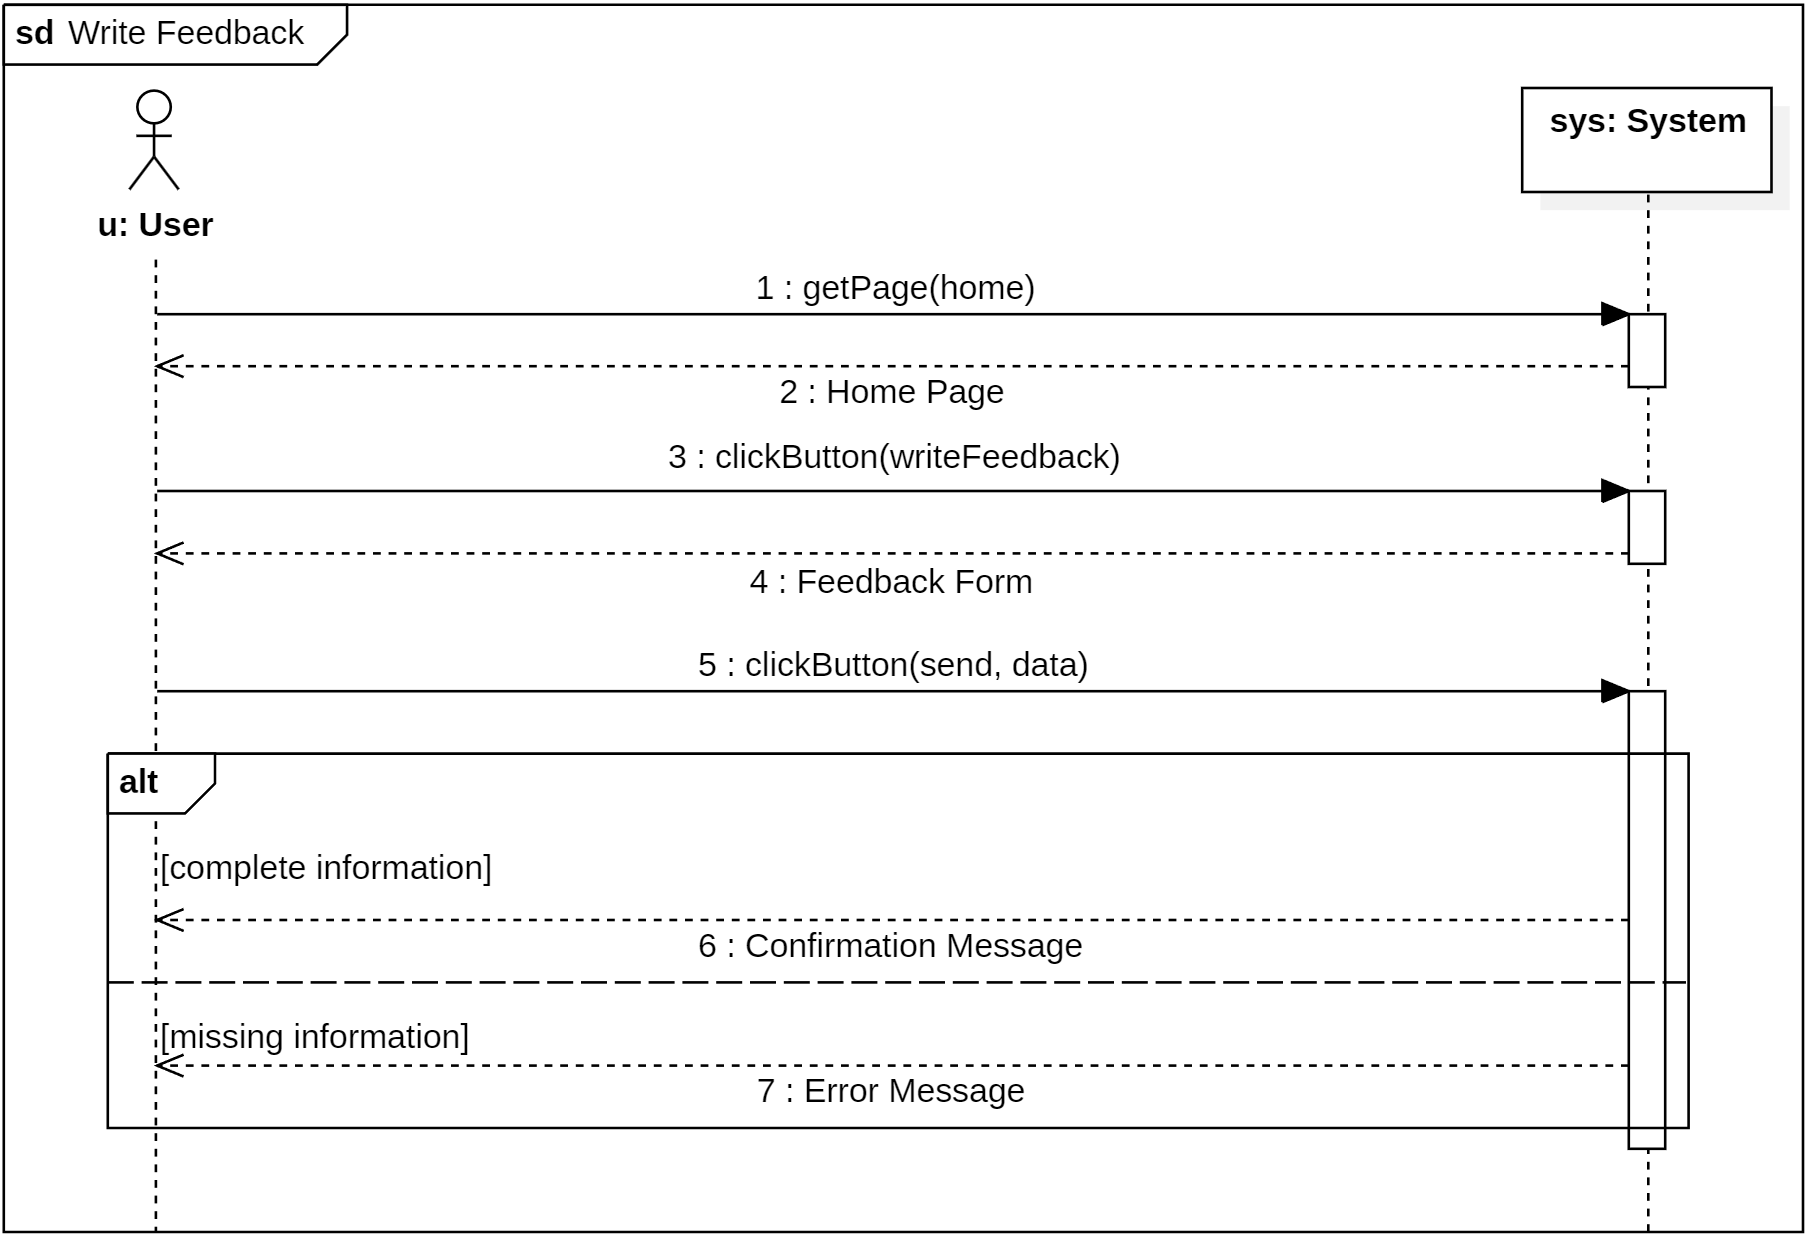
\includegraphics[width=1\linewidth]{Use Cases Images/write_feedback.png}
    \caption{Diagram for [UC14]}
    \label{fig: Write Feedback Diagram}
\end{figure}

\subsubsection*{Write Complaint}
\begin{table}[H]
    \centering
    \renewcommand{\arraystretch}{1.5}
    \begin{tabular}{|p{4cm}|p{11cm}|}
    \hline
    \rowcolor{bluepoli!40}
    \textbf{[UC15]} & \textbf{Writes Complaint} \\ \hline \hline
    \textbf{Actors} & Student, University \\ \hline
    \textbf{Entry Condition} & 
    {\setlength{\leftmargini}{1.1em}
    \begin{itemize}
        \item The student is registered on the platform.
        \item The student is logged in.
        \item The student is currently involved in an ongoing internship.
    \end{itemize}} \\ \hline
    \textbf{Input} & Details of the complaint (e.g., description of the issue, affected parties, date, etc.). \\ \hline
    \textbf{Event Flow} & 
    {\setlength{\leftmargini}{1.4em}
    \begin{enumerate}
        \item The student navigates to the internship page.
        \item The student clicks on the "Write Complaint" button.
        \item The system displays the complaint form.
        \item The student fills in the complaint details.
        \item The student clicks on the "Send" button.
        \item The university receives a notification about the new complaint.
    \end{enumerate}} \\ \hline
    \textbf{Exit Condition} & 
    {\setlength{\leftmargini}{1.1em}
    \begin{itemize}
        \item The new complaint is successfully saved in the system.
        \item The university is notified.
    \end{itemize}} \\ \hline
    \textbf{Output} & Confirmation message to the student that the complaint has been submitted successfully. \\ \hline
    \textbf{Exceptions} & / \\ \hline
    \end{tabular}
    \caption{Write Complaint Table}
\end{table}

\begin{figure} [H]
    \centering
    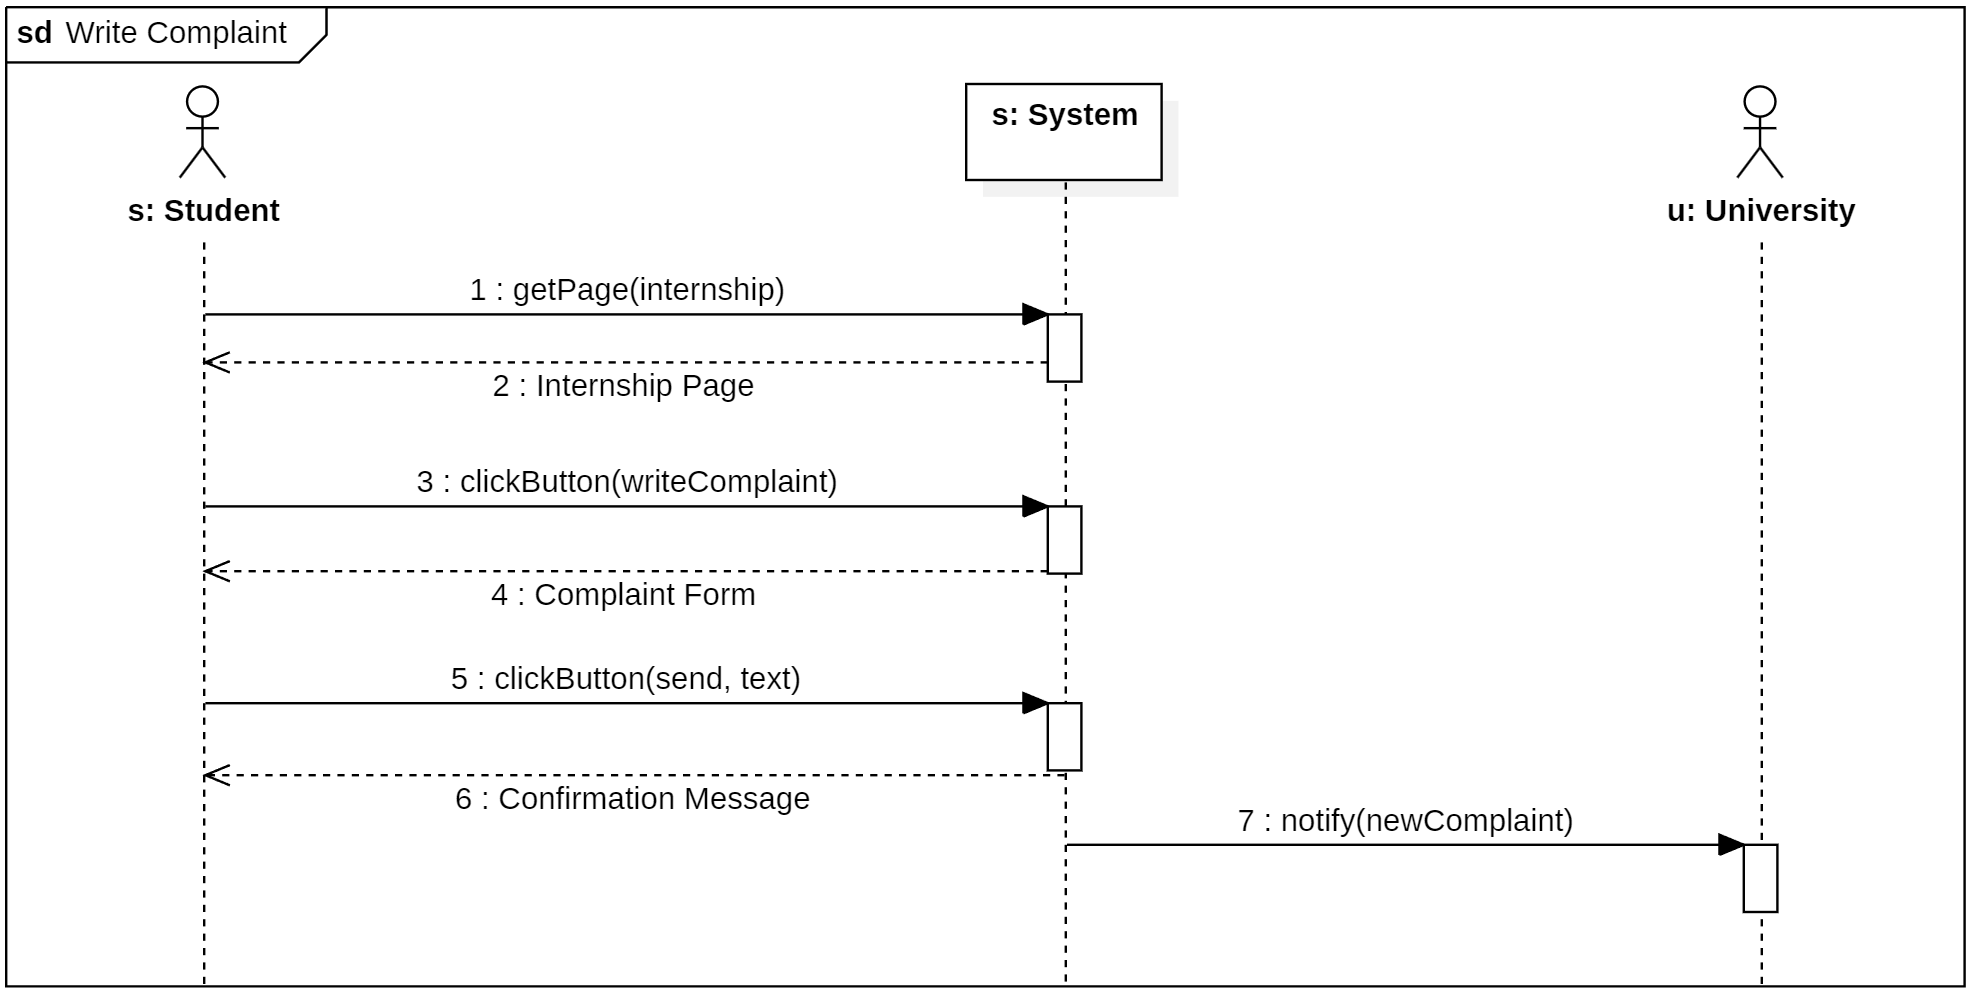
\includegraphics[width=1\linewidth]{Use Cases Images/write_complaint.png}
    \caption{Diagram for [UC15]}
    \label{fig: Write Complaint Diagram}
\end{figure}

\subsubsection*{Handle Complaint}
\begin{table}[H]
    \centering
    \renewcommand{\arraystretch}{1.5}
    \begin{tabular}{|p{4cm}|p{11cm}|}
    \hline
    \rowcolor{bluepoli!40}
    \textbf{[UC16]} & \textbf{Handle Complaints} \\ \hline \hline
    \textbf{Actors} & University, Student, Company \\ \hline
    \textbf{Entry Condition} & 
    {\setlength{\leftmargini}{1.1em}
    \begin{itemize}
        \item The university has a student that is currently involved in an internship.
    \end{itemize}} \\ \hline
    \textbf{Input} & Reply to the complaint. \\ \hline
    \textbf{Event Flow} & 
    {\setlength{\leftmargini}{1.4em}
    \begin{enumerate}
        \item The university opens the complaints page on the platform.
        \item The university clicks on the "Manage" button of a specific complaint to handle.
        \item The system displays the complaint options.
        \item The university handles/replies to the complaint.
        \item The university clicks "Submit" to send the reply to the involved parties.
    \end{enumerate}} \\ \hline
    \textbf{Exit Condition} & 
    {\setlength{\leftmargini}{1.1em}
    \begin{itemize}
        \item The complaint has been handled.
        \item The reply to the complaint has been sent to the involved parties.
    \end{itemize}} \\ \hline
    \textbf{Output} & 
    Confirmation message to the university that the reply to the complaint has been submitted successfully. \\ \hline
    \textbf{Exceptions} & 
    {\setlength{\leftmargini}{1.1em}
    \begin{itemize}
        \item \textbf{No Complaints Available:} If no complaints are available, the system displays a message indicating that there are no complaints to handle.
    \end{itemize}} \\ \hline
    \end{tabular}
    \caption{Handle Complaint Table}
\end{table}

\begin{figure} [H]
    \centering
    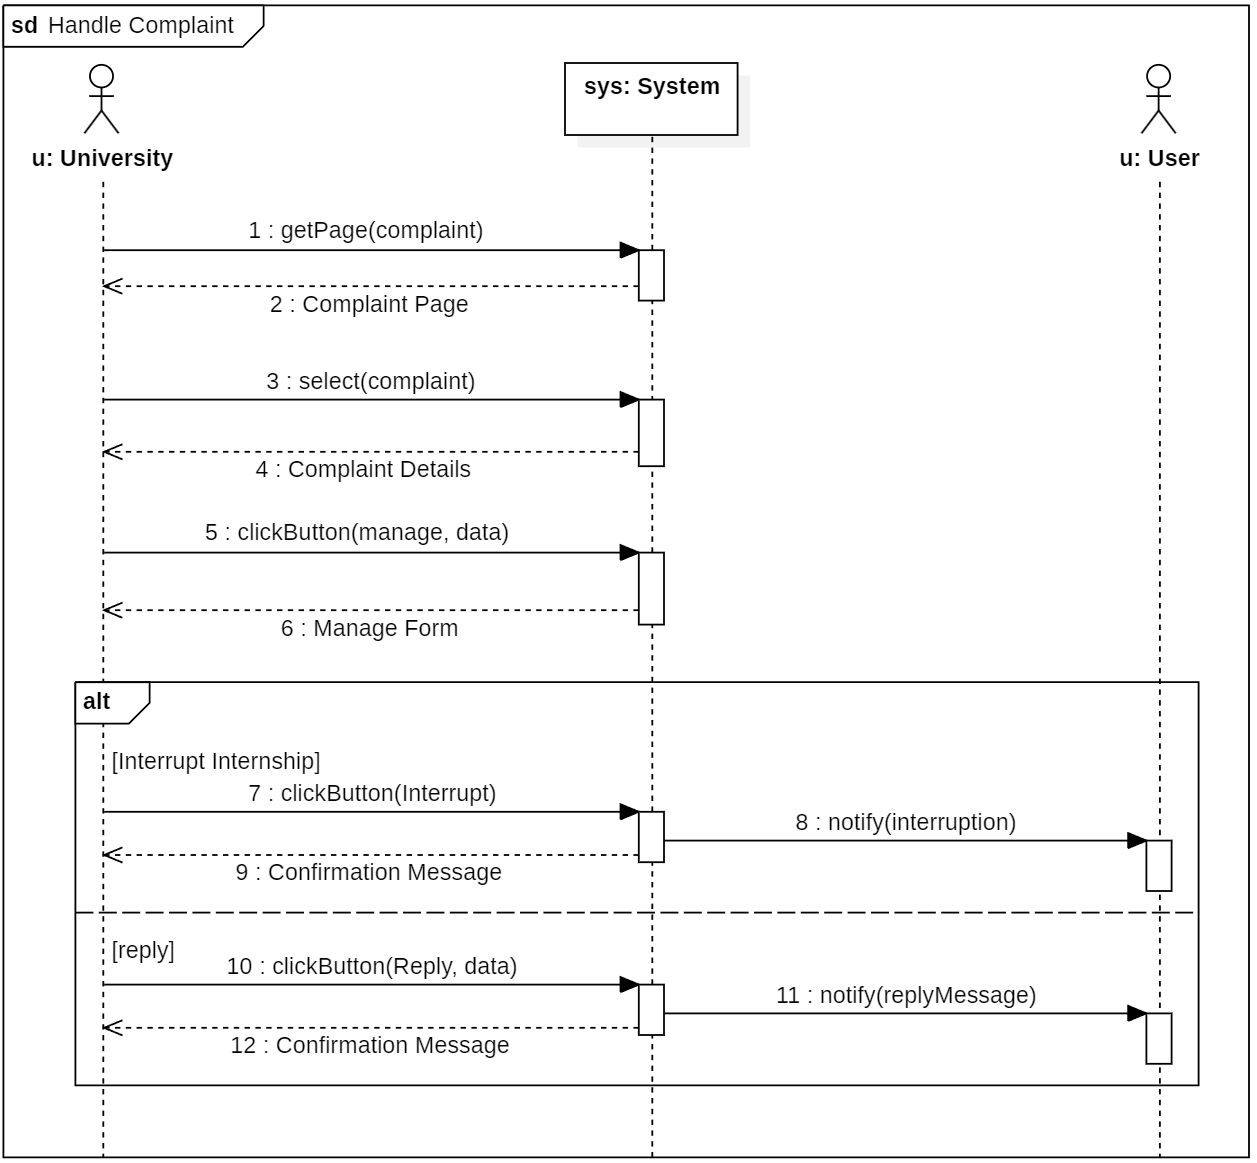
\includegraphics[width=1\linewidth]{Use Cases Images/handle_complaint.png}
    \caption{Diagram for [UC16]}
    \label{fig: Handle Complaint Diagram}
\end{figure}

\newpage
\subsection{Requirements mapping}

This section offers a brief summary of the objectives, clearly defining the specific requirements and underlying assumptions related to each goal.

\textbf{[G1]} Allow students to look for internships and stay updated about new opportunities
\begin{itemize}
    \item \textbf{R1} - The system allows unregistered users to sign up
    \item \textbf{R2} -The system allows users to log in
    \item \textbf{R8} - The system takes information from the student's personal profile
    \item \textbf{R9} - The system allows a student to see a company’s profile
    \item \textbf{R13} - The system displays all the available internships 
    \item \textbf{R14} - The system displays all the information of each specific internship
    \item \textbf{R15} - The system displays specific internships that better suit a student based on the information provided
    \item \textbf{R25} - The system asks users for permission to send messages
    \item \textbf{D1} - User must consent to personal data extraction and usage
    \item \textbf{D2} - User must consent to receiving information
    \item \textbf{D3} - User must have a device able to connect to the internet
    \item \textbf{D4} - Student must be enrolled in a university
\end{itemize}

\textbf{[G2]} Allow students to improve their CVs
\begin{itemize}
    \item \textbf{R3} - The system allows students to insert personal information for the creation of the CV
    \item \textbf{R5} - The system allows users to update their personal profiles
    \item \textbf{R7} - the system allows users to retrieve all modified information
    \item \textbf{R29} - The system generates suggestions based on the information taken in the platform
    \item \textbf{D1} - Student must be enrolled in a university
    \item \textbf{D2} - User must have a device able to connect to the internet
\end{itemize}

\textbf{[G3]} Allow students to apply for an internship
\begin{itemize}
    \item \textbf{R16} - The system allows students to visualize information about the internship
    \item \textbf{R17} - The system allows a registered student to select an internship to apply to
    \item \textbf{R18} - The system allows users to apply to an internship
    \item \textbf{R26} - The system generates a message of confirmation after the operation is done
    \item \textbf{D1} - User must consent to personal data extraction and usage
    \item \textbf{D2} - User must consent to receiving information
    \item \textbf{D3} - User must have a device able to connect to the internet
    \item \textbf{D4} - Student must be enrolled in a university
\end{itemize}

\textbf{[G4]} Allow a company to hire interns
\begin{itemize}
    \item \textbf{R1} - The system allows unregistered users to sign up
    \item \textbf{R2} -The system allows users to log in
    \item \textbf{R6} - The system allows companies to view student's personal profile
    \item \textbf{R10} - The system changes the status of evaluation after updates in the
    \item \textbf{R19} - The system allows companies to set up evaluation criteria application process
    \item \textbf{D1} - User must consent to personal data extraction and usage
    \item \textbf{D2} - User must consent to receiving information
    \item \textbf{D3} - User must have a device able to connect to the internet
\end{itemize}

\textbf{[G5]} Allow companies to improve their internship proposals
\begin{itemize}
    \item \textbf{R4} - The system allows companies to insert information for the creation of the internship
    \item \textbf{R5} - The system allows users to update their personal profiles
    \item \textbf{R7} - The system allows users to retrieve all modified information
    \item \textbf{R29} - The system generates suggestions based on the information taken in the platform
    \item \textbf{D1} - User must have a device able to connect to the internet
\end{itemize}

\textbf{[G6]} Allow users to track and monitor the status of the internship
\begin{itemize}
    \item \textbf{R10} - The system changes the status of evaluation after updates in the application process
    \item \textbf{R11} - The system allows students to accept the outcome of the evaluation
    \item \textbf{R12} - The system allows companies to evaluate students’applications
    \item \textbf{R25} - The system asks users for permission to send messages
    \item \textbf{R27} - The system generates a message once the status of the internship changes
    \item \textbf{D1} - User must consent to personal data extraction and usage
    \item \textbf{D2} - User must consent to receiving information
    \item \textbf{D3} - User must have a device able to connect to the internet
    \item \textbf{D4} - Student must be enrolled in a university
\end{itemize}

\textbf{[G7]} Allow users to report feedback and complaints
\begin{itemize}
    \item \textbf{R21} - The system allows users to name other parties involved in the complaint
    \item \textbf{R22} - The system asks users for permission to send messages
    \item \textbf{R26} - The system generates a message of confirmation after the operation is done
    \item \textbf{R28} - The system allows user to retrieve all messages sent 
    \item \textbf{R30} - The system allows students and companies to provide feedback
    \item \textbf{R31} - The system generated a feedback request to send to students and companies
    \item \textbf{D1} - User must have a device able to connect to the internet
    \item \textbf{D2} - Student must be enrolled in a university
\end{itemize}

\textbf{[G8]} Allow universities to review and address complaints
\begin{itemize}
    \item \textbf{R1} - The system allows unregistered users to sign up
    \item \textbf{R2} -The system allows users to log in
    \item \textbf{R20} - The system allows universities to set up criteria for internship's conclusion
    \item \textbf{R22} - The system displays the complaints sent by both students and companies
    \item \textbf{R23} - The system updates the status of a complaint
    \item \textbf{R24} - The system allows universities to close an internship
    \item \textbf{D1} - Student must be enrolled in a university
\end{itemize}



\section{Performance Requirements}

The system must guarantee high performance to support a large number of users, including students, companies, and universities, while ensuring a smooth and seamless user experience. To achieve this, the system is expected to exhibit a swift response time, ideally no more than one second, to prevent delays that might hinder students from submitting applications or companies from managing internships effectively. In cases where the user’s Internet connection is slow, response times may increase noticeably. In addition, the system must efficiently handle interactions such as CV generation, internship recommendations, and feedback management while ensuring smooth and seamless processing of data. The manageable workload of the platform is supported by its focussed scope, as complex operations such as interviews and submissions rely on predefined data structures rather than real-time computation.

\section{Design Constraints}

\subsection{Regulatory Polices}

The system guarantees accessibility and cross-browser compatibility by adhering to open web standards (HTML, CSS, and JavaScript). It complies with data protection regulations such as the GDPR and CCPA to handle data securely. The platform meets WCAG accessibility standards and ensures consistent performance across browsers like Chrome, Firefox, Safari, and Edge.

\subsection{Hardware Limitations}

All that is required in terms of hardware is a computer with an internet connection.

\subsection{Other Constraints}

There are no other specific requirements needed for the use of the platform.

\section{Software System Attributes}

\subsection{Reliability}
The system should reduce downtime to the greatest extent possible, enabling users to continuously search for new opportunities and track all necessary information without interruption.

\subsection{Availability}
Availability is important, and the system must ensure 98\% uptime to guarantee that users can access the platform whenever needed.

\subsection{Security}
Security is critical for the system due to the sensitive personal information it handles. As such, all operations are designed to be authorized. Encryption and the SSL protocol ensure a secure communication channel. Additionally, the system adheres to security standards, including those set by the Open Web Application Security Project (OWASP), to protect against common web application vulnerabilities such as SQL injection, cross-site request forgery (CSRF), and cross-site scripting (XSS).

\subsection{Maintainability}
The system will be developed following the best software engineering practices to ensure its maintainability and scalability over time. It is designed to facilitate the integration of future functionalities with minimal effort, allowing easy expansion. The selected design techniques will focus on ensuring a high level of reusability, making it easier to adapt the system as new requirements emerge.

\subsection{Portability}
The system is engineered with a focus on easy portability, ensuring it can adapt to changes in hosting databases or hardware components. Designed to be fully compatible with most operational systems, it also offers accessibility through any web browser. This flexibility ensures the system remains highly portable. Moving forward, it is crucial to maintain compatibility with future updates, as well as any new operating systems or devices.






\chapter{Formal analysis using Alloy}

Here we present the specification of the system described above using Alloy. The goal of this specification is to model a system that ensures the integrity and correctness of constraints related to internship applications, student eligibility, and system behaviors.

The specification is structured around a set of signatures: users, students, companies, internships, and universities. Each entity is defined with its attributes and relationships. For instance, students are modeled as users with additional attributes like their applied internships, current internship work, CV, and associated university.

Facts are also introduced to define constraints. These includes that no two users can share the same email, a student cannot apply for an internship without a CV, and only one student can work in a given internship at a time. Additional constraints verify that students can only be rejected from internships they have previously applied to, and historical rules ensure that a CV always belongs to a single student throughout the system's lifecycle.

We used predicates to define dynamic operations such as students applying for internships, starting work, or being rejected. A global "eventsFact" encapsulates the control flow of these operations to maintain consistency within the system.

Finally, a world predicate establishes initial conditions for the system, such as ensuring there are more than two students, companies, and internships in the environment

\vspace{2cm}
\lstinputlisting[language=alloy]{Alloy/RASD_ALLOY.als}

\subsubsection*{Examples}

In this scenario, there are two companies: one is offering three internships, while the other is offering a single internship. We also have three students studying at the same university.

\begin{figure} [H]
    \centering
    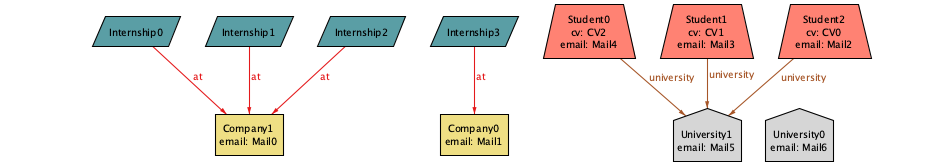
\includegraphics[width=1\linewidth]{Alloy/State.png}
    \caption{State 0}
\end{figure}

At the first step Student0 applies for Internship0.

\begin{figure} [H]
    \centering
    \includegraphics[width=1\linewidth]{Alloy/State1.png}
    \caption{State 1}
\end{figure}

At the second step, Student2 applies for Internship1 but gets rejected.

\begin{figure} [H]
    \centering
    \includegraphics[width=1\linewidth]{Alloy/State2.png}
    \caption{State 2}
\end{figure}

At the third step, Student0 applies for Internship3 while Student2 applies for Intership0

\begin{figure} [H]
    \centering
    \includegraphics[width=1\linewidth]{Alloy/State3.png}
    \caption{State 3}
\end{figure}

At the fourth step, Student0 gets accepted and starts working on Internship3. 

\begin{figure} [H]
    \centering
    \includegraphics[width=1\linewidth]{Alloy/State4.png}
    \caption{State 4}
\end{figure}

At the fifth step, Student2's application to Internship0 gets rejected.

\begin{figure} [H]
    \centering
    \includegraphics[width=1\linewidth]{Alloy/State5.png}
    \caption{State 5}
\end{figure}

At the sixth step, Student1 applies for Internship0

\begin{figure} [H]
    \centering
    \includegraphics[width=1\linewidth]{Alloy/State6.png}
    \caption{State 6}
\end{figure}

\chapter{Effort spent}

\chapter{Reference}
In the RASD-Document we have used the following references:
\newline
Websites that have a similar use case:
\begin{itemize}
    \item \textbf{LeetCode}
    \item \textbf{GitHub}
\end{itemize}

Websites used for the mockups:
\begin{itemize}
    \item \textbf{Figma}
\end{itemize}

Websites used for the diagrams:
\begin{itemize}
    \item \textbf{StarUML}
\end{itemize}



%-------------------------------------------------------------------------
%	BIBLIOGRAPHY
%-------------------------------------------------------------------------

\addtocontents{toc}{\vspace{2em}} % Add a gap in the Contents, for aesthetics
%\bibliography{Thesis_bibliography} % The references information are stored in the file named "Thesis_bibliography.bib"

%-------------------------------------------------------------------------
%	APPENDICES
%-------------------------------------------------------------------------

\cleardoublepage
\addtocontents{toc}{\vspace{2em}} % Add a gap in the Contents, for aesthetics
\chapter*{Appendix A}
\label{chapter:Appendix A}
Appendix A

If you want to include a pdf file:
%\includepdf[pages=-,pagecommand=\thispagestyle{empty},]{filetitle.pdf}


\cleardoublepage

%\input{Instructions.tex}


\end{document}
